%=======================================================================
%  DAS732: Data Visualization / Term 1 (2026-27) / Programming Assignment 1
%  International Institute of Information Technology Bangalore
%
%  Build:  pdflatex DAS732_A1_Report.tex   (run 3x for ToC + cross-refs)
%     or:  latexmk -pdf DAS732_A1_Report.tex
%     or:  python ../code/build_report_pdf.py   (wraps latexmk and checks the log)
%
%  Figures are read from ../images/ and are produced by the scripts in ../code/.
%=======================================================================
\documentclass[11pt,a4paper]{article}

\usepackage[T1]{fontenc}
\usepackage[utf8]{inputenc}
\usepackage{lmodern}
\usepackage{microtype}
\usepackage[a4paper,top=2.3cm,bottom=2.4cm,left=2.2cm,right=2.2cm]{geometry}

\usepackage{graphicx}
\graphicspath{{../images/}}
\usepackage{float}
\usepackage{booktabs}
\usepackage{tabularx}
\usepackage{array}
\usepackage{longtable}
\usepackage{multirow}
\usepackage{enumitem}
\usepackage{xcolor}
\usepackage{amsmath}
\usepackage[font=small,labelfont=bf,labelsep=period,
            justification=justified,singlelinecheck=false]{caption}
\usepackage{fancyhdr}
\usepackage{titlesec}
\usepackage[hidelinks,breaklinks=true]{hyperref}
\usepackage{pdfpages}   % appends the signed AI declarations

%----------------------------------------------------------------- colours --
% Same palette as the figures, so the document reads as one piece of design.
\definecolor{inkblue}{HTML}{2A78D6}
\definecolor{inkorange}{HTML}{EB6834}
\definecolor{inkgrey}{HTML}{52514E}
\definecolor{inkmuted}{HTML}{8A8985}
\definecolor{rulegrey}{HTML}{E3E2DE}
\definecolor{bandgrey}{HTML}{F4F3EF}

\hypersetup{
  colorlinks=false,
  pdftitle={DAS732 A1 -- A Century of Natural Disasters},
  pdfsubject={Visual exploration of the EM-DAT Emergency Events Database, 1900--2022},
  pdfkeywords={data visualization, EM-DAT, natural disasters, Tableau, DAS732}
}

%------------------------------------------------------------------ layout --
\titleformat{\section}{\normalfont\Large\bfseries\sffamily}{\thesection}{0.7em}{}
\titleformat{\subsection}{\normalfont\large\bfseries\sffamily\color{inkblue}}{\thesubsection}{0.6em}{}
\titleformat{\subsubsection}{\normalfont\normalsize\bfseries\sffamily}{\thesubsubsection}{0.6em}{}
\titlespacing*{\section}{0pt}{2.2ex plus 1ex minus .2ex}{1.2ex plus .2ex}
\titlespacing*{\subsection}{0pt}{1.8ex plus 1ex minus .2ex}{0.9ex plus .2ex}

\pagestyle{fancy}
\fancyhf{}
\renewcommand{\headrulewidth}{0pt}
\renewcommand{\footrulewidth}{0.4pt}
\renewcommand{\footrule}{\color{rulegrey}\hrule height 0.4pt \vspace{2pt}}
\fancyfoot[L]{\footnotesize\color{inkmuted}\sffamily DAS732 A1 $\cdot$ EM-DAT Natural Disasters, 1900--2022}
\fancyfoot[R]{\footnotesize\color{inkmuted}\sffamily\thepage}

\setlength{\parskip}{0.55em}
\setlength{\parindent}{0pt}
\renewcommand{\arraystretch}{1.25}
\setlist[itemize]{leftmargin=1.3em,itemsep=0.25em,topsep=0.3em}
\setlist[enumerate]{leftmargin=1.6em,itemsep=0.25em,topsep=0.3em}

% A boxed callout for the guiding question and the headline answer.
\newcommand{\callout}[1]{%
  \begin{center}\vspace{0.2em}
  \colorbox{bandgrey}{%
    \begin{minipage}{0.955\linewidth}
      \vspace{0.6em}
      {\color{inkblue}\rule{2.5pt}{1em}}\hspace{0.6em}%
      \begin{minipage}{0.93\linewidth}#1\end{minipage}
      \vspace{0.6em}
    \end{minipage}}
  \vspace{0.2em}\end{center}}

% One knob for every figure's scale. Figures are wide, so a little
% under \linewidth lets two task blocks share a page instead of
% leaving a third of each page blank.
\newcommand{\figw}{\linewidth}

% Shorthand used throughout the figure sections.
\newcommand{\inference}{\textbf{Inference.}\ }
\newcommand{\rationale}{\textbf{Rationale.}\ }
\newcommand{\howto}{\textbf{How to read it.}\ }
\newcommand{\taskhead}[2]{\subsection*{Task #1 --- #2}%
  \addcontentsline{toc}{subsection}{Task #1 --- #2}}

%------------------------------------------------------------ team names --
% EDIT THESE SIX LINES ONLY - every occurrence in the document follows them.
% Using macros also avoids the classic LaTeX trap in which a table row that
% literally begins with "[" is swallowed as an optional argument to \\.
\newcommand{\memberA}{Lakshya Jain}
\newcommand{\rollA}{BT2024044}
\newcommand{\memberB}{Arnav Jain}
\newcommand{\rollB}{BT2024233}
\newcommand{\memberC}{Kalpit}
\newcommand{\rollC}{BT2024093}

%=======================================================================
\begin{document}
%=======================================================================

%------------------------------------------------------------ title page --
\begin{titlepage}
\thispagestyle{empty}
\raggedright
\vspace*{0.4cm}

{\color{inkmuted}\sffamily\large DAS732: Data Visualization \quad$\cdot$\quad Term 1 (2026--27)\par}
{\color{inkmuted}\sffamily\large International Institute of Information Technology Bangalore\par}

\vspace{0.75cm}
{\color{rulegrey}\rule{\linewidth}{1.2pt}}
\vspace{0.65cm}

{\sffamily\bfseries\fontsize{24}{29}\selectfont
A Century of Natural Disasters:\\[0.22em]
More Events, Fewer Deaths, Bigger Bills\par}

\vspace{0.5cm}
{\sffamily\Large\color{inkgrey}
Visual Exploration of the EM-DAT Emergency\\Events Database, 1900--2022\par}

\vspace{0.55cm}
{\color{rulegrey}\rule{\linewidth}{1.2pt}}
\vspace{0.65cm}

{\sffamily\large\textbf{Programming Assignment 1 (A1)}\\[0.25em]
{\color{inkgrey}Visual Exploration Using Visual Analytics Tools}\par}

\vspace{0.6cm}

{\sffamily
\begin{tabular}{@{}ll@{}}
\textbf{Dataset allotted} & \#7 --- Natural Disasters Emergency Events Database\\
                          & (EM-DAT based, 1900--2022)\\[0.3em]
\textbf{Team size}        & 3 members\\[0.3em]
\textbf{Submission}       & 13 September 2026\\
\end{tabular}\par}

\vspace{0.75cm}

{\sffamily\large\textbf{Team and task allocation}\par}
\vspace{0.3em}
{\small
\begin{tabularx}{\linewidth}{@{}>{\raggedright\arraybackslash}p{4.0cm}
                               >{\raggedright\arraybackslash}p{2.6cm} X@{}}
\toprule
\textbf{Member} & \textbf{Roll number} & \textbf{Task set}\\
\midrule
\memberA & \rollA & \textbf{A} --- \emph{When?} The temporal record
  (Figures \ref{fig:types}--\ref{fig:trimmed}), plus data preprocessing\\
\memberB & \rollB & \textbf{B} --- \emph{Where?} The geography of exposure
  (Figures \ref{fig:mapevents}--\ref{fig:lethality})\\
\memberC & \rollC & \textbf{C} --- \emph{What?} The impact signature of
  hazards (Figures \ref{fig:signature}--\ref{fig:decoupling})\\
\bottomrule
\end{tabularx}}

\vspace{0.85cm}
\callout{\small\textbf{Note on AI use.} A signed AI declaration for each team
member is included at the end of this report (Section~\ref{sec:ai}), on the form
circulated by the course instructor. The verification harness described in
Section~\ref{sec:repro} documents how every number in this report was
independently re-derived from the raw data.}
\end{titlepage}

%------------------------------------------------------------------ front --
\clearpage
\tableofcontents
\vspace{1.2em}
\listoffigures
\vspace{1.2em}
\listoftables
\clearpage

%=======================================================================
\section{Introduction and Guiding Question}
%=======================================================================

Public conversation about natural disasters usually runs on a single intuition:
that the world is being hit harder every year. The EM-DAT Emergency Events
Database, which has catalogued disaster events country by country since 1900, is
the standard evidence base for testing that intuition. This assignment uses it to
answer one question through visualization.

\callout{\textbf{Guiding question.} Over 1900--2022, has the burden of natural
disasters actually grown, and has the world become better or worse at surviving
it?}

The question is deliberately compound, because a disaster has no single cost. An
event can be \emph{counted}, it can \emph{kill}, it can \emph{displace}, and it
can \emph{destroy property}, and those four measures need not move together. The
question therefore decomposes into the three sub-questions of
Table~\ref{tab:subq}, each owned end to end by one team member so that no task is
fragmented across the team. Figure~\ref{fig:taskmap} shows that decomposition and
how the three strands converge on a single data story.

\begin{table}[H]
\centering
\caption{The guiding question decomposed into three independently owned
sub-questions. Ownership is by whole task set, never by individual chart.}
\label{tab:subq}
\small
\begin{tabularx}{\linewidth}{@{}c X >{\raggedright\arraybackslash}p{1.9cm}
                               >{\raggedright\arraybackslash}p{2.0cm}@{}}
\toprule
& \textbf{Sub-question} & \textbf{Owner} & \textbf{Figures}\\
\midrule
\textbf{A} & \textbf{When?} How has the recorded burden changed over time --- and
how much of that change is real rather than an artefact of record-keeping?
& Member 1 & \ref{fig:types}--\ref{fig:trimmed}\\
\textbf{B} & \textbf{Where?} Where does the burden fall, and does the country that
records the most disasters also suffer the most harm?
& Member 2 & \ref{fig:mapevents}--\ref{fig:lethality}\\
\textbf{C} & \textbf{What?} Which hazards kill, which displace, and which cost
money --- and are they the same hazards?
& Member 3 & \ref{fig:signature}--\ref{fig:decoupling}\\
\bottomrule
\end{tabularx}
\end{table}

Each sub-question is answered by a \emph{sequence} of visualization tasks rather
than by a single chart, and the three sequences are designed to converge on one
data story, set out in Section~\ref{sec:story}.

\subsection{Visualization tasks}

Tasks are labelled using the descriptive verbs of the design space of Schulz et
al.~\cite{schulz2013}: \emph{overview, trend, locate, rank, compare, relate,
derive, correlate, identify, validate}. Table~\ref{tab:tasks} lists the fifteen
tasks. Each figure in Sections~\ref{sec:taskA}--\ref{sec:taskC} is introduced by
the task it implements, the rationale for the chart form chosen, and the
inference drawn from it.

\begin{table}[H]
\centering
\caption{The fifteen visualization tasks, their Schulz et al.\ verbs, and the
figure that implements each one.}
\label{tab:tasks}
\small
\begin{tabularx}{\linewidth}{@{}>{\raggedright\arraybackslash}p{1.4cm} X
                               >{\raggedright\arraybackslash}p{3.5cm}
                               >{\raggedright\arraybackslash}p{1.6cm}@{}}
\toprule
\textbf{Task} & \textbf{Description} & \textbf{Verb(s)} & \textbf{Figure}\\
\midrule
A1.1 & Characterise the composition of the record & Overview, Summarize & \ref{fig:types}\\
A1.2 & Trace recorded events through time & Trend & \ref{fig:trend}\\
A1.3 & Test whether the trend is real or a reporting artefact & Identify, Validate & \ref{fig:reporting}\\
A1.4 & Contrast total mortality against mortality per event & Compare, Derive & \ref{fig:deaths}\\
A1.5 & Test whether the mortality decline is broad-based & Validate, Derive & \ref{fig:trimmed}\\
\addlinespace
B1.1 & Locate disaster occurrence on the globe & Locate, Overview & \ref{fig:mapevents}\\
B1.2 & Locate disaster mortality on the globe & Locate, Compare & \ref{fig:mapdeaths}\\
B1.3 & Rank countries on four separate burdens & Rank, Compare & \ref{fig:leaderboards}\\
B1.4 & Quantify how concentrated each burden is & Derive, Compare & \ref{fig:concentration}\\
B1.5 & Derive lethality with exposure held roughly constant & Derive, Rank & \ref{fig:lethality}\\
\addlinespace
C1.1 & Compare each hazard's share of four burdens & Compare, Summarize & \ref{fig:signature}\\
C1.2 & Relate a hazard's deadliness to its cost & Relate, Locate & \ref{fig:scatter}\\
C1.3 & Trace real economic damage through time & Trend & \ref{fig:damage}\\
C1.4 & Compare lethality change across hazards and decades & Compare, Trend & \ref{fig:heatmap}\\
C1.5 & Correlate the four burdens on one indexed scale & Correlate, Trend & \ref{fig:decoupling}\\
\bottomrule
\end{tabularx}
\end{table}

\subsection{Tasks considered and rejected}
\label{sec:rejected}

The brief asks for the tasks we \emph{tried} as well as those we eventually
implemented. Six candidate tasks were prototyped and dropped, each for a reason
that is itself a finding about the dataset.

\begin{enumerate}
\item \textbf{Deaths per million population, by country.} The natural way to
  compare countries fairly. Dropped because the file carries no population
  column; supplying one would mean joining an external source with a different
  vintage and country list, which we judged out of scope for a single-dataset
  assignment. Task B1.5 (Figure~\ref{fig:lethality}) is the substitute: it holds
  \emph{exposure} roughly constant instead of population, by restricting to the
  20 countries with the most recorded events.
\item \textbf{Damage as a share of GDP.} Same problem as population, and the same
  resolution: damage is reported per event and per decade in constant dollars
  instead.
\item \textbf{Epidemics and pandemics.} Attempted, then abandoned on inspection:
  the \texttt{Biological} sub-group in this file contains only 92 insect
  infestations and one animal accident. There are no epidemic rows at all, so no
  honest task can be built on them.
\item \textbf{Sub-type analysis} (25 sub-types, e.g.\ riverine flood versus flash
  flood). Prototyped and dropped: 20.4\% of rows carry no sub-type, and the
  missingness is concentrated in the early decades. A sub-type time series would
  therefore have shown a spurious ``rise of flash floods'' that is really the
  arrival of finer classification. The analysis stays at the 13-type level, where
  coverage is complete.
\item \textbf{A country $\times$ hazard-type matrix.} Built as a clustered
  heatmap, then dropped: with 225 countries it is unreadable at report scale and
  violates the brief's requirement for plots a layman can read. Its one useful
  finding is stated in text instead --- of the 132 countries with at least 20
  recorded events, flood is the most frequent hazard in 82 and storm in 39.
\item \textbf{A choropleth of deaths per event.} Dropped because countries with
  one or two recorded events produce extreme, meaningless ratios that dominate
  the colour scale. Figure~\ref{fig:lethality} shows the same measure as a ranked
  bar chart over a filtered, comparable set of countries.
\end{enumerate}

Two further presentation ideas were rejected on principle rather than on data: a
dual-axis chart pairing deaths with damage (see Section~\ref{sec:method}), and an
animated time slider, which cannot survive into a static PDF and is instead part
of the Tableau demo.

\begin{figure}[H]
\centering
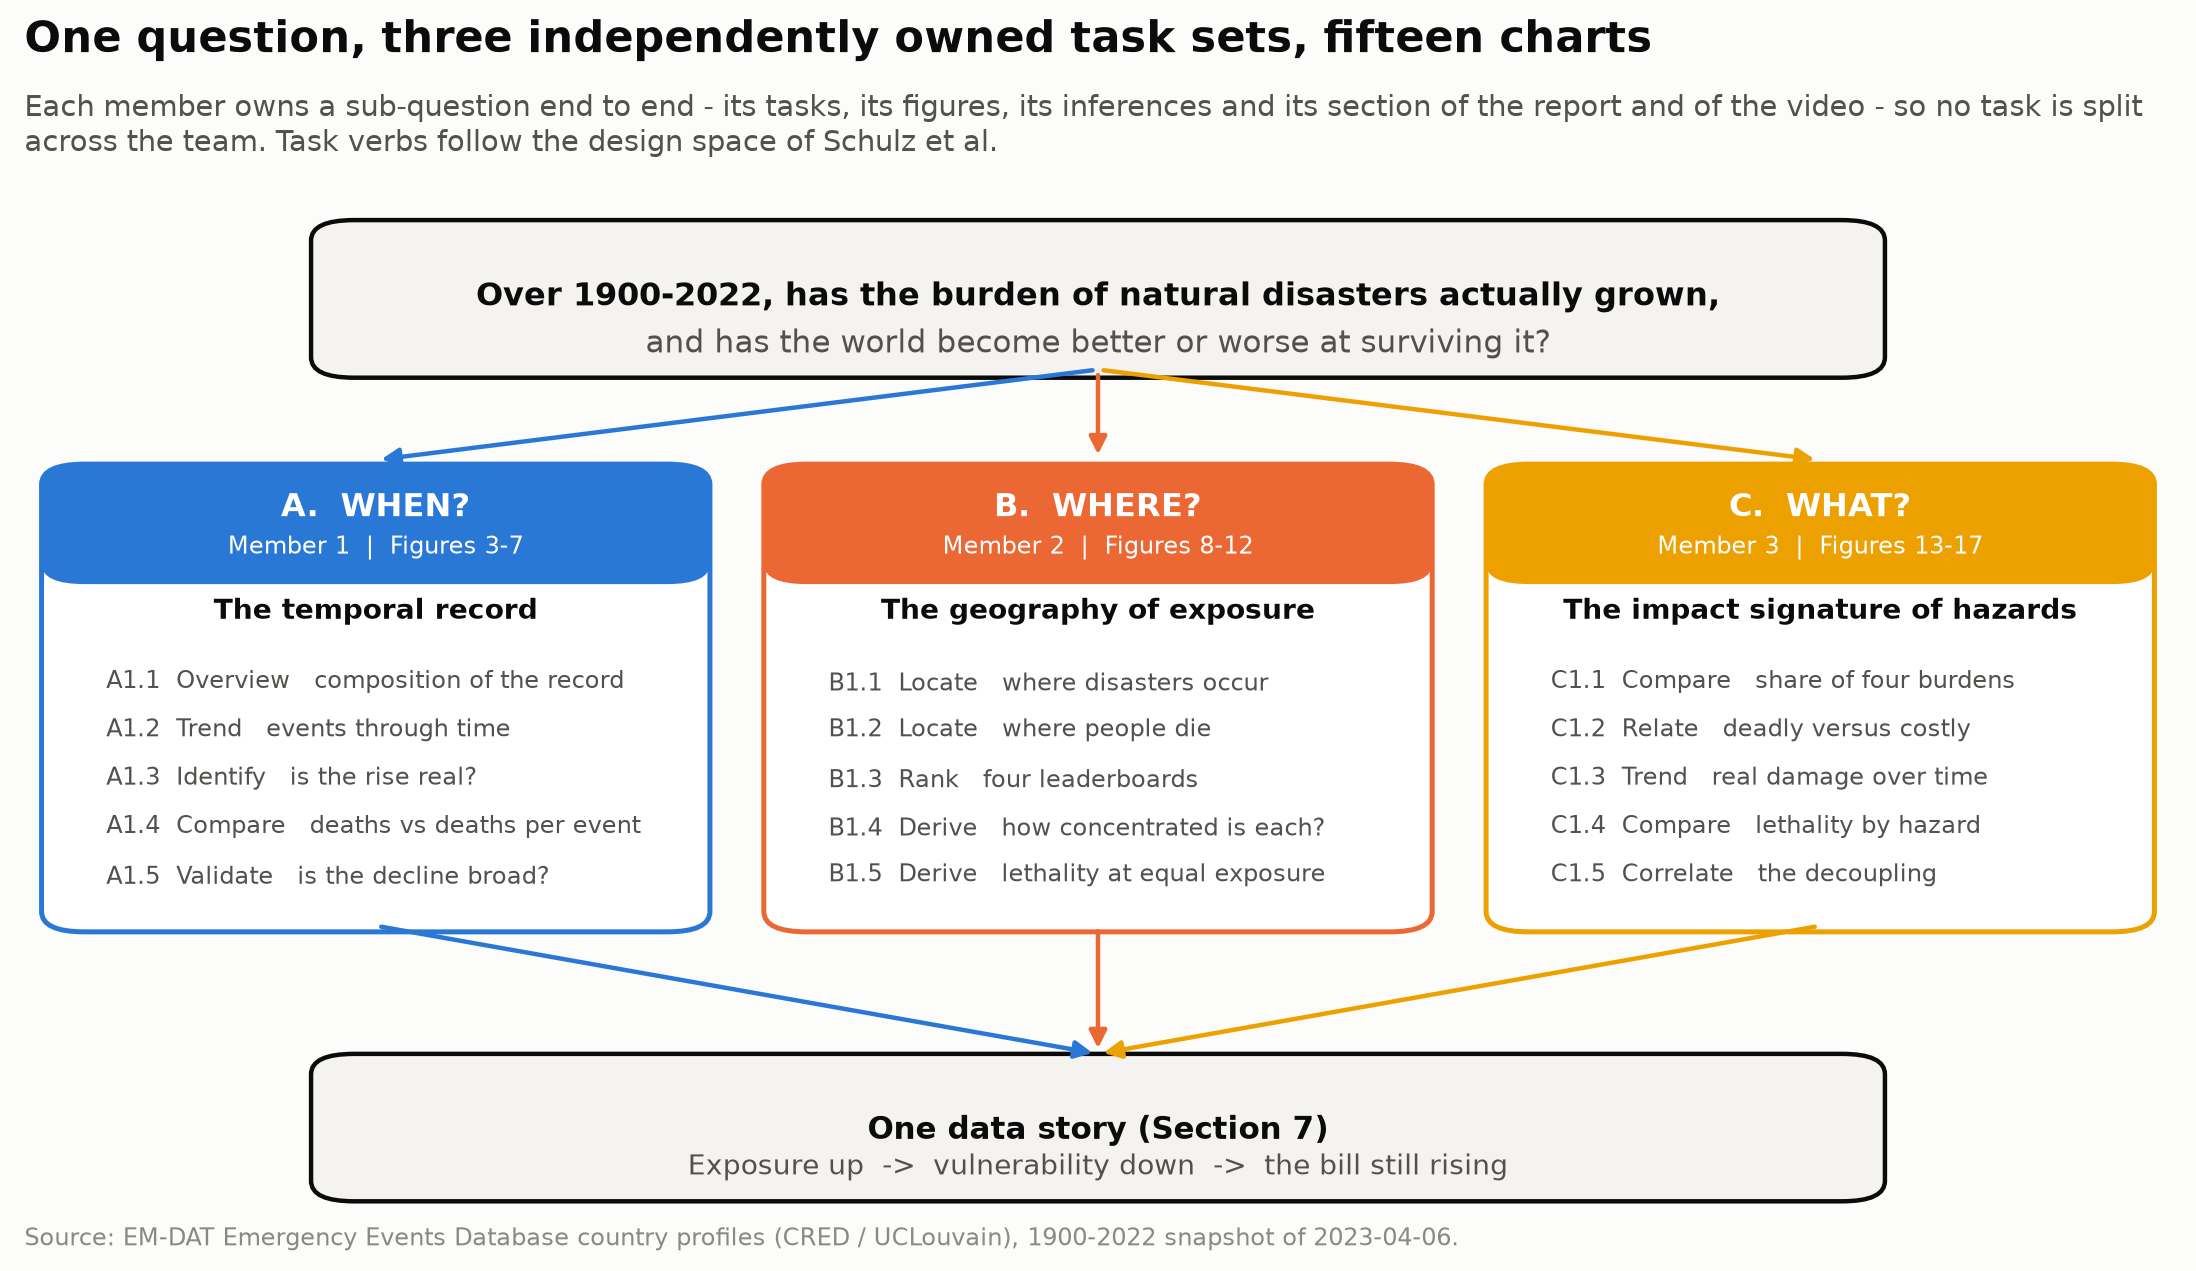
\includegraphics[width=\figw]{Fig1}
\caption[Task decomposition: one question, three task sets]{\textbf{Task
decomposition.} One guiding question, three independently owned task sets,
fifteen charts, one data story. Ownership is by whole sub-question so that each
member's contribution is separable and equal, as the assignment brief requires.}
\label{fig:taskmap}
\end{figure}

\howto The box at the top is the single guiding question. The three columns
below it are the three task sets; each is headed by a coloured band naming the
member who owns it and the figures they produced, and lists that member's five
tasks with the Schulz et al.\ verb each one implements. The arrows run downward
only: the question splits into three independent strands, and the three strands
converge on the single data story at the foot of the diagram. Nothing crosses
sideways between columns, which is the point --- no task is shared.

%=======================================================================
\section{Dataset Description}
%=======================================================================

\subsection{Source and provenance}

The file used is the \textbf{country-profiles} export of EM-DAT, the Emergency
Events Database maintained by the Centre for Research on the Epidemiology of
Disasters (CRED) at UCLouvain, Brussels~\cite{emdat}, distributed on Kaggle as
\emph{Natural Disasters Emergency Events Database}~\cite{kaggle}. The single CSV
in that dataset is
%
\begin{quote}\ttfamily\small
\_EmergencyEventsDatabase-CountryProfiles\_emdat-country-profiles\_2023\_04\_06.csv
\end{quote}
%
a snapshot taken on \textbf{6 April 2023}. It is semicolon-delimited and uses a
comma as the decimal mark, so it must be read with
\texttt{sep=';', decimal=','}; read with defaults, every numeric column arrives
as text.

A row is \textbf{not} one disaster. A row is one \emph{(year, country, disaster
type, disaster subtype)} combination, with the number of events in that
combination held in \texttt{Total Events}. There are \textbf{10{,}431 rows}
describing \textbf{15{,}015 recorded events}.

\subsection{Schema}

Table~\ref{tab:schema} lists the thirteen columns, the variable type of each and
how often it is missing. The dataset spans all four variable types the brief asks
for: temporal (\texttt{Year}), categorical (five nested hazard fields),
numerical (four impact measures) and geospatial (\texttt{Country} /
\texttt{ISO}).

\begin{table}[H]
\centering
\caption{Schema of the raw file, with the variable type of each column and the
share of rows in which it is missing.}
\label{tab:schema}
\small
\begin{tabularx}{\linewidth}{@{}>{\raggedright\arraybackslash}p{4.3cm}
                               >{\raggedright\arraybackslash}p{2.2cm} X
                               >{\raggedleft\arraybackslash}p{1.5cm}@{}}
\toprule
\textbf{Column} & \textbf{Type} & \textbf{Description} & \textbf{Missing}\\
\midrule
\texttt{Year} & Temporal (ordinal) & 1900--2023 & 0\%\\
\texttt{Country} & Categorical (nominal) & 225 distinct countries and territories & 0\%\\
\texttt{ISO} & Categorical (nominal) & ISO-3166 alpha-3 code; the join key for the maps & 0\%\\
\texttt{Disaster Group} & Categorical & Always \texttt{Natural}; no technological disasters & 0\%\\
\texttt{Disaster Subroup} & Categorical & 5 values: Hydrological, Meteorological, Geophysical, Climatological, Biological \emph{(the column name is misspelled in the source file)} & 0\%\\
\texttt{Disaster Type} & Categorical & 13 values, e.g.\ Flood, Storm, Earthquake, Drought & 0\%\\
\texttt{Disaster Subtype} & Categorical & 25 values, e.g.\ Riverine flood, Tropical cyclone, Ground movement & 20.4\%\\
\texttt{Total Events} & Numerical (count) & Events in that year/country/type/subtype cell; 1--20 & 0\%\\
\texttt{Total Affected} & Numerical (count) & People injured, made homeless, or requiring assistance & 27.3\%\\
\texttt{Total Deaths} & Numerical (count) & Deaths and missing presumed dead & 29.3\%\\
\texttt{Total Damage (USD, original)} & Numerical (currency) & Damage in the prices of the year of the event & 63.2\%\\
\texttt{Total Damage (USD, adjusted)} & Numerical (currency) & Damage in constant 2022 US dollars & 63.2\%\\
\texttt{CPI} & Numerical (index) & Price index used for the adjustment; 2.85 (1900) to 100.00 (2022) & 0.5\%\\
\bottomrule
\end{tabularx}
\end{table}

Missing percentages are quoted for the raw 10{,}431-row file. In the
10{,}380-row analysis frame the \texttt{CPI} column is complete, because the 51
rows that lacked it are exactly the 51 partial-year 2023 rows that are dropped.

We verified the relationship between the two damage columns rather than assuming
it. Across all rows where both are present,
\[
  \texttt{Total Damage (adjusted)} \;=\;
  \texttt{Total Damage (original)} \times \frac{100}{\texttt{CPI}}
\]
holds to within $2.5\times10^{-4}$, and $\texttt{CPI}=100$ exactly in 2022.
\textbf{The adjusted column is therefore constant 2022 US dollars, and it is the
only damage measure used in this report.} Comparing nominal dollars across a
123-year span would have made the trend in Figure~\ref{fig:damage} almost
entirely an artefact of inflation: the nominal total is \$4.19 trillion against a
real total of \$6.70 trillion.

\subsection{Preprocessing}
\label{sec:prep}

All cleaning is performed in one shared module, \texttt{code/emdat\_common.py},
so that the three task sets are guaranteed to be working from an identical
frame. Figure~\ref{fig:pipeline} shows the pipeline; Table~\ref{tab:prep} lists
the rules and the reason for each.

\begin{figure}[H]
\centering
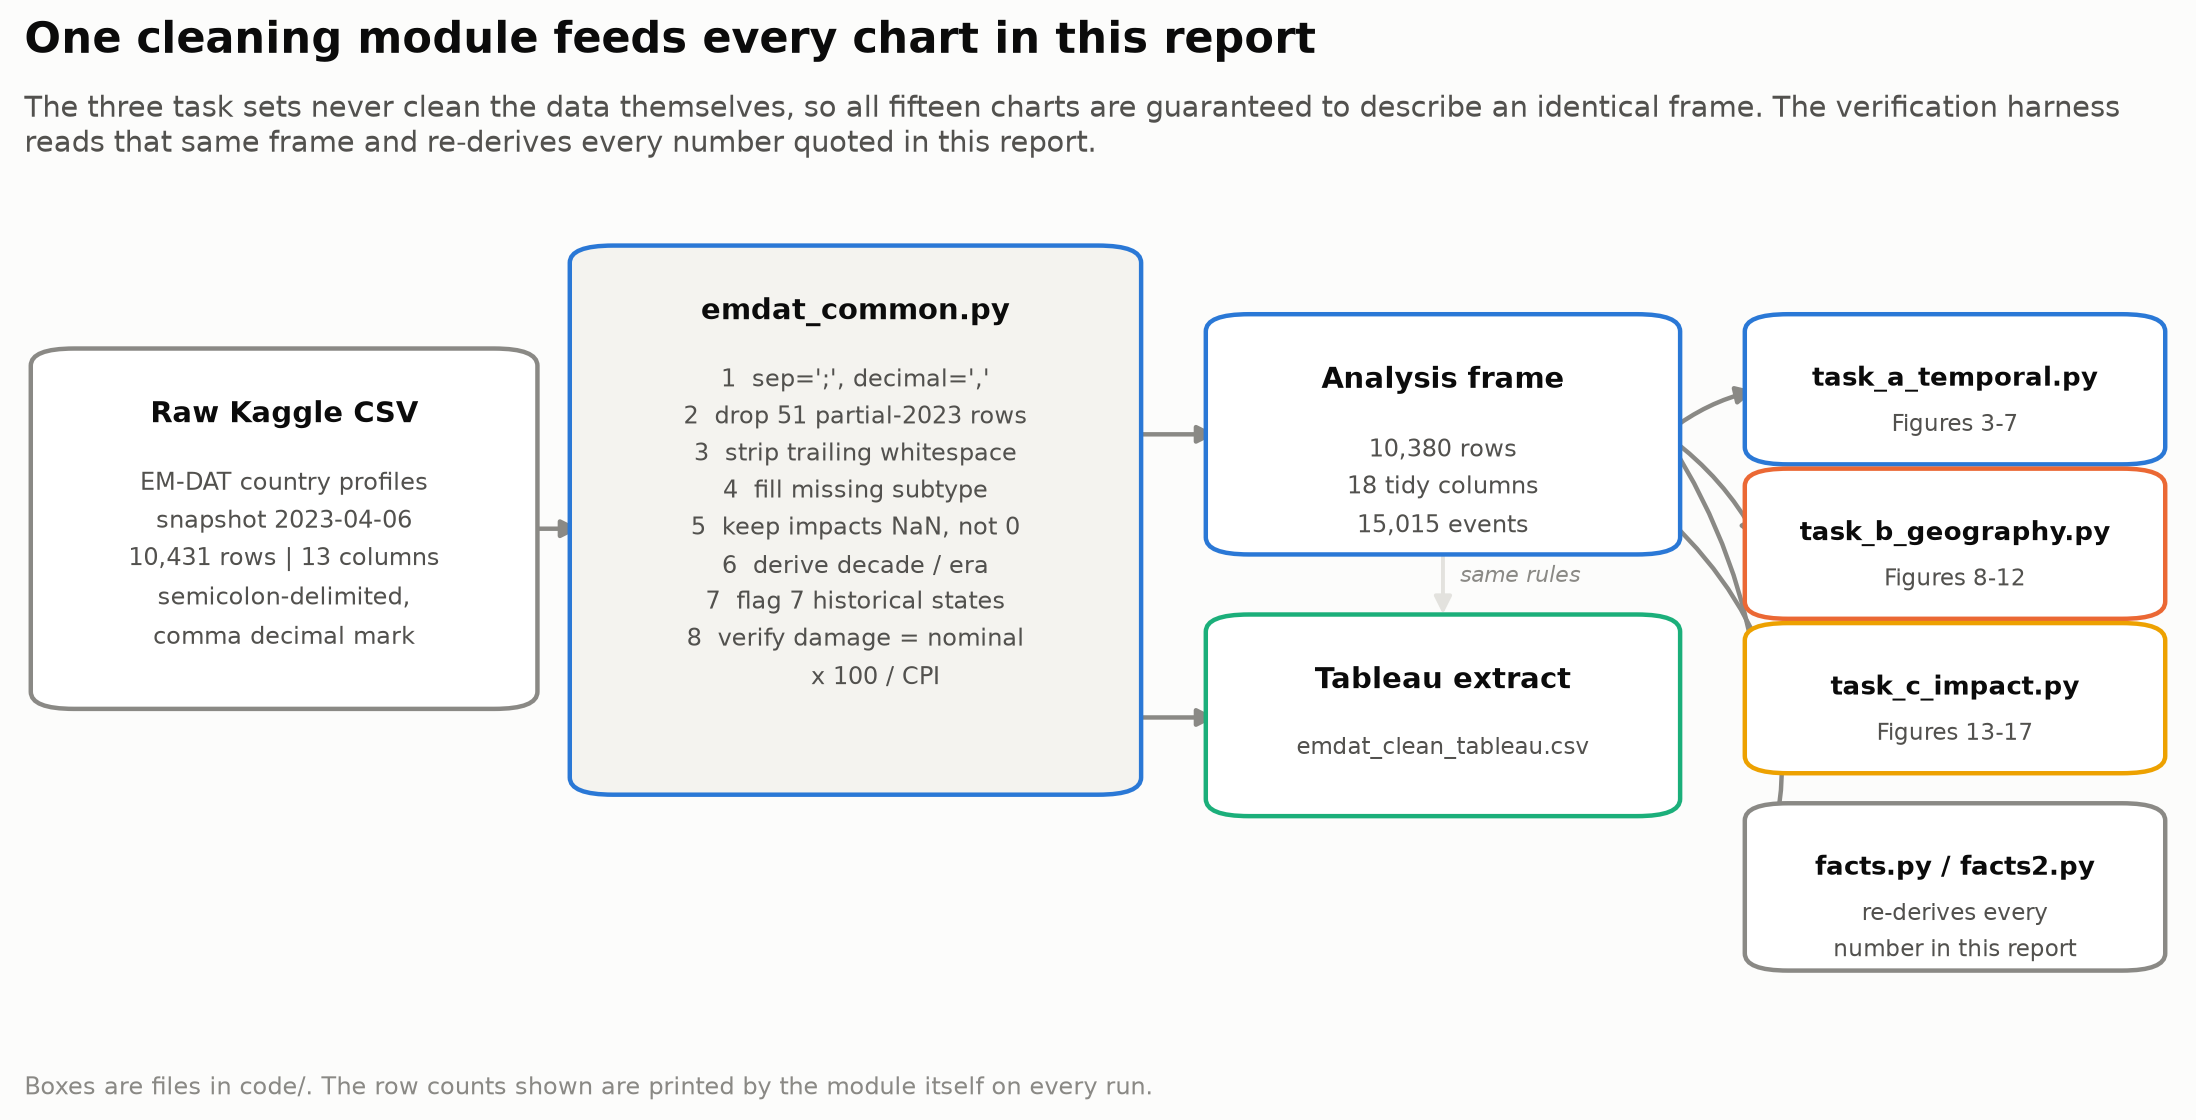
\includegraphics[width=\figw]{Fig2}
\caption[Data pipeline from raw CSV to figures]{\textbf{The processing
pipeline.} A single cleaning module produces the analysis frame and the
Tableau extract; the three task-set scripts and the verification harness all
read that same frame, so no chart in this report can be describing a
differently-cleaned dataset.}
\label{fig:pipeline}
\end{figure}

\howto Read left to right; every box is a file in the submission and every
arrow is data moving. The grey box on the left is the raw download, exactly as
Kaggle supplies it. The large blue box is the one cleaning module, with its eight
numbered rules listed in the order they are applied. It emits two things: the
in-memory analysis frame used by the charts, and the flat CSV used by Tableau ---
the small grey arrow between them marks that both come from identical rules. The
four boxes on the right are the scripts that consume the frame; the three upper
ones are labelled with the figures they generate, and the fourth is the
verification harness.

\begin{table}[H]
\centering
\caption{Preprocessing rules applied in \texttt{emdat\_common.py}, their effect
on the data, and the reason each is necessary.}
\label{tab:prep}
\small
\begin{tabularx}{\linewidth}{@{}c >{\raggedright\arraybackslash}p{3.5cm}
                               >{\raggedright\arraybackslash}p{3.3cm} X@{}}
\toprule
\textbf{\#} & \textbf{Rule} & \textbf{Effect} & \textbf{Why}\\
\midrule
1 & Read with \texttt{sep=';'}, \texttt{decimal=','} & Numeric columns parse correctly & European CSV conventions; otherwise every measure is a string\\
2 & Drop rows dated 2023 & $-51$ rows $\rightarrow$ \textbf{10{,}380 rows} & The snapshot is dated 6 April 2023, so 2023 is a fractional year that would fake a collapse in every trend. All 51 rows also have a null CPI, confirming they are incomplete\\
3 & Strip whitespace from all label columns & 13 hazard types, not 14 & The source carries a trailing space on some \texttt{Disaster Type} values (\texttt{"Extreme temperature~"}), silently splitting one category in two\\
4 & Fill missing \texttt{Disaster Subtype} with \texttt{"<Type> (unspecified)"} & 2{,}133 rows retained & EM-DAT records only a coarse type for older events; dropping them would bias the record toward recent years\\
5 & Leave impact columns as \texttt{NaN}, never zero & Per-event severity stays honest & Zero-filling would treat ``not reported'' as ``nobody died'', understating historical severity\\
6 & Derive \texttt{decade} and a 1900--1969 / 1970--2022 \texttt{era} flag & Used by Figures \ref{fig:reporting}, \ref{fig:deaths}, \ref{fig:trimmed}, \ref{fig:damage}, \ref{fig:heatmap} & Decadal aggregation suppresses single-year noise\\
7 & Flag 7 historical states no longer in existence & Soviet Union, Czechoslovakia, Yugoslavia, Germany Dem Rep, Serbia Montenegro, Yemen Arab Rep, Yemen P Dem Rep & These appear in the country rankings (Figure~\ref{fig:leaderboards}) and must be read as historical entities, not present-day countries\\
8 & Emit the cleaned Tableau extract
    \texttt{data/}\allowbreak\texttt{emdat\_clean\_}\allowbreak\texttt{tableau.csv} & 10{,}380 rows, 18 tidy columns & A flat, Tableau-ready extract needing no further cleaning\\
\bottomrule
\end{tabularx}
\end{table}

\subsection{Known limitations of the source}
\label{sec:sourcelimits}

These constrain what can honestly be claimed, and are revisited in
Section~\ref{sec:limits}.

\begin{enumerate}
\item \textbf{Reporting bias.} 90.6\% of all recorded events fall in 1970--2022,
  a span covering only 43.1\% of the 123 years. Event counts before about 1970
  measure historical record-keeping at least as much as they measure hazard.
\item \textbf{Damage under-reporting.} Only 36.9\% of records carry a damage
  figure, so every damage total here is a lower bound.
\item \textbf{No population denominator.} The file has no population column, so
  ``deaths per event'' is used as the severity measure rather than deaths per
  capita. A large country will record more events than a small one for reasons
  of area and population alone.
\item \textbf{No epidemics.} The \texttt{Biological} sub-group in this file
  contains only insect infestations (92 rows) and one animal accident. There are
  no epidemic or pandemic rows, so COVID-19 and comparable events are entirely
  absent.
\item \textbf{Aggregated rows.} Because a row can hold up to 20 events, per-event
  figures are averages over a cell, not properties of individual disasters.
\end{enumerate}

%=======================================================================
\section{Method and Design Conventions}
\label{sec:method}
%=======================================================================

Every figure in this report follows one set of rules, so that a reader who learns
to read the first chart can read all fifteen.

\begin{itemize}
\item \textbf{Colour has one job per chart.} Categorical palettes encode identity
  (hazard type, sub-group) with a fixed slot order that never changes between
  figures --- \emph{Hydrological} is the same blue in Figure~\ref{fig:trend} and
  Figure~\ref{fig:damage}. Sequential single-hue blue ramps encode magnitude
  (Figures~\ref{fig:mapevents}, \ref{fig:mapdeaths}, \ref{fig:heatmap}). No
  rainbow scales are used.
\item \textbf{Colour-vision safety was computed, not judged.} The five-colour
  categorical palette was run through a colour-vision-deficiency separation
  check before use; the worst adjacent pair scores $\Delta E = 9.1$ under
  protanopia against a target of $\geq 8$, and every value shown on a
  light-coloured fill carries a visible text label, so colour is never the only
  channel.
\item \textbf{No dual-axis charts.} Where two measures of different scale must be
  compared, they are drawn as two stacked panels sharing an $x$-axis
  (Figure~\ref{fig:deaths}) or indexed to a common base
  (Figure~\ref{fig:decoupling}). A twin $y$-axis lets the author choose the
  crossing point and is therefore avoided.
\item \textbf{Log scales are labelled as such} and are used only where the data
  span three or more orders of magnitude.
\item \textbf{Every chart states its own finding in its title.} The chart title
  is the inference; the chart subtitle carries the caveat.
\item \textbf{Every figure is explained in the same three steps}, so a reader can
  understand any figure without having read the ones before it. The
  \emph{caption} says what the figure is and why that chart form was chosen;
  \textbf{How to read it} decodes the picture itself --- what is on each axis,
  what the marks, colours and sizes encode, whether a scale is logarithmic, and
  what the annotations mark; and \textbf{Inference} states what the figure
  demonstrates. Where a figure needed justifying before it could be believed, a
  \textbf{Rationale} paragraph precedes the inference.
\item \textbf{Part-decade warning.} The 2020s bucket holds only 2020--2022 and is
  annotated wherever it appears.
\end{itemize}

%=======================================================================
\section{Task Set A --- \emph{When?} The Temporal Record}
\label{sec:taskA}
%=======================================================================

\textbf{Owner:} \memberA \quad$\cdot$\quad
\textbf{Figures:} \ref{fig:types}--\ref{fig:trimmed} \quad$\cdot$\quad
\textbf{Script:} \texttt{code/task\_a\_temporal.py}

\taskhead{A1.1}{Overview: what is in the record?}

\begin{figure}[H]
\centering
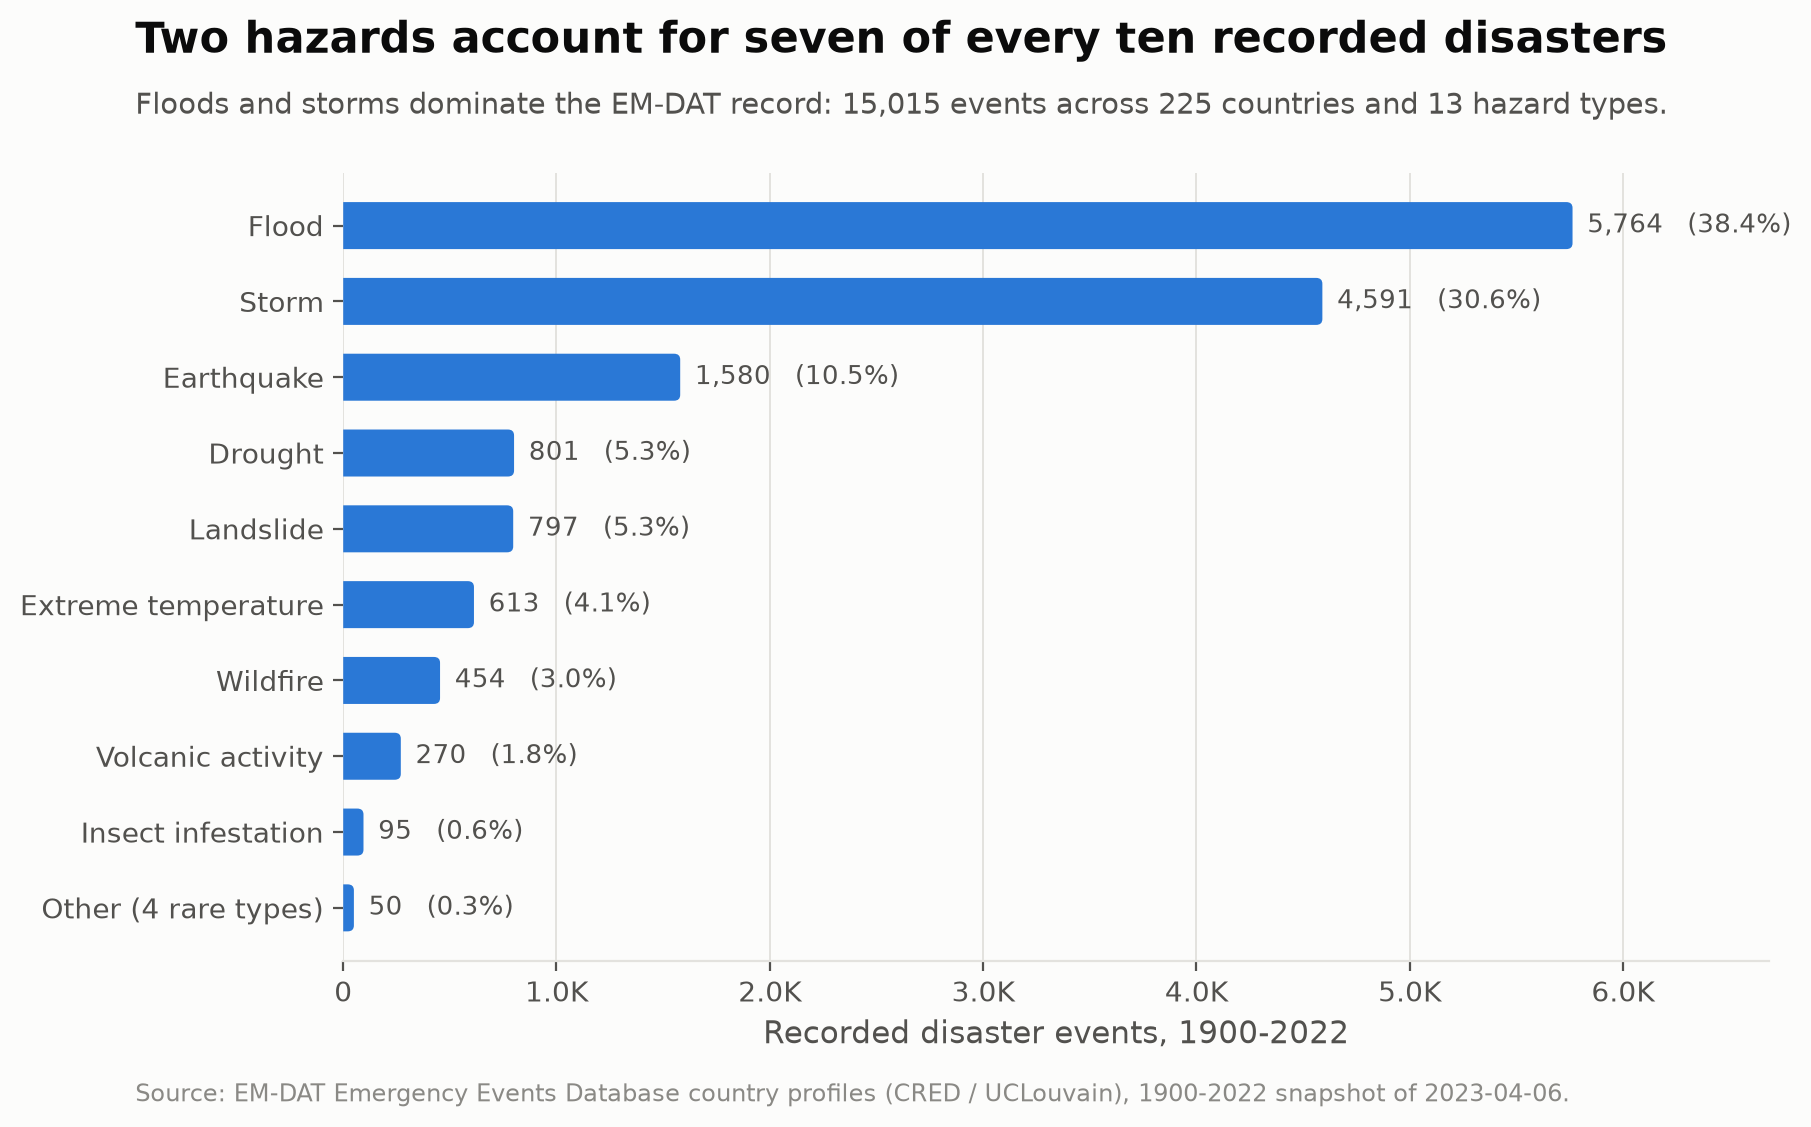
\includegraphics[width=\figw]{Fig3}
\caption[Recorded events by hazard type]{\textbf{Recorded disaster events by
hazard type, 1900--2022.} A horizontal bar chart is used because the category
labels are long words that read naturally on the $y$-axis, and because rank is
the question being asked. The four rarest types (mass movement, glacial lake
outburst, fog, animal accident --- 50 events combined) are folded into
``Other'' rather than being given their own colours.}
\label{fig:types}
\end{figure}

\howto One horizontal bar per hazard type. Bar length is the total number of
events recorded for that hazard across 1900--2022, and the number and percentage
at the end of each bar give the exact value, so nothing has to be estimated off
the axis. Bars are sorted longest-first. The bottom bar, ``Other'', aggregates
the four rarest types (mass movement, glacial lake outburst, fog and animal
accident) because individually each is too small to see.

\inference The record is dominated by water and weather. Floods (5{,}764 events,
38.4\%) and storms (4{,}591, 30.6\%) together account for \textbf{69\% of all
recorded events}. Earthquakes are a distant third at 10.5\%. Drought --- which
Task Set C will show to be by far the deadliest hazard --- accounts for only
5.3\% of events. The first finding of the report is therefore that
\emph{frequency and harm are different questions}, and the rest of the analysis
follows that split.

\taskhead{A1.2}{Trend: when were these events recorded?}

\begin{figure}[H]
\centering
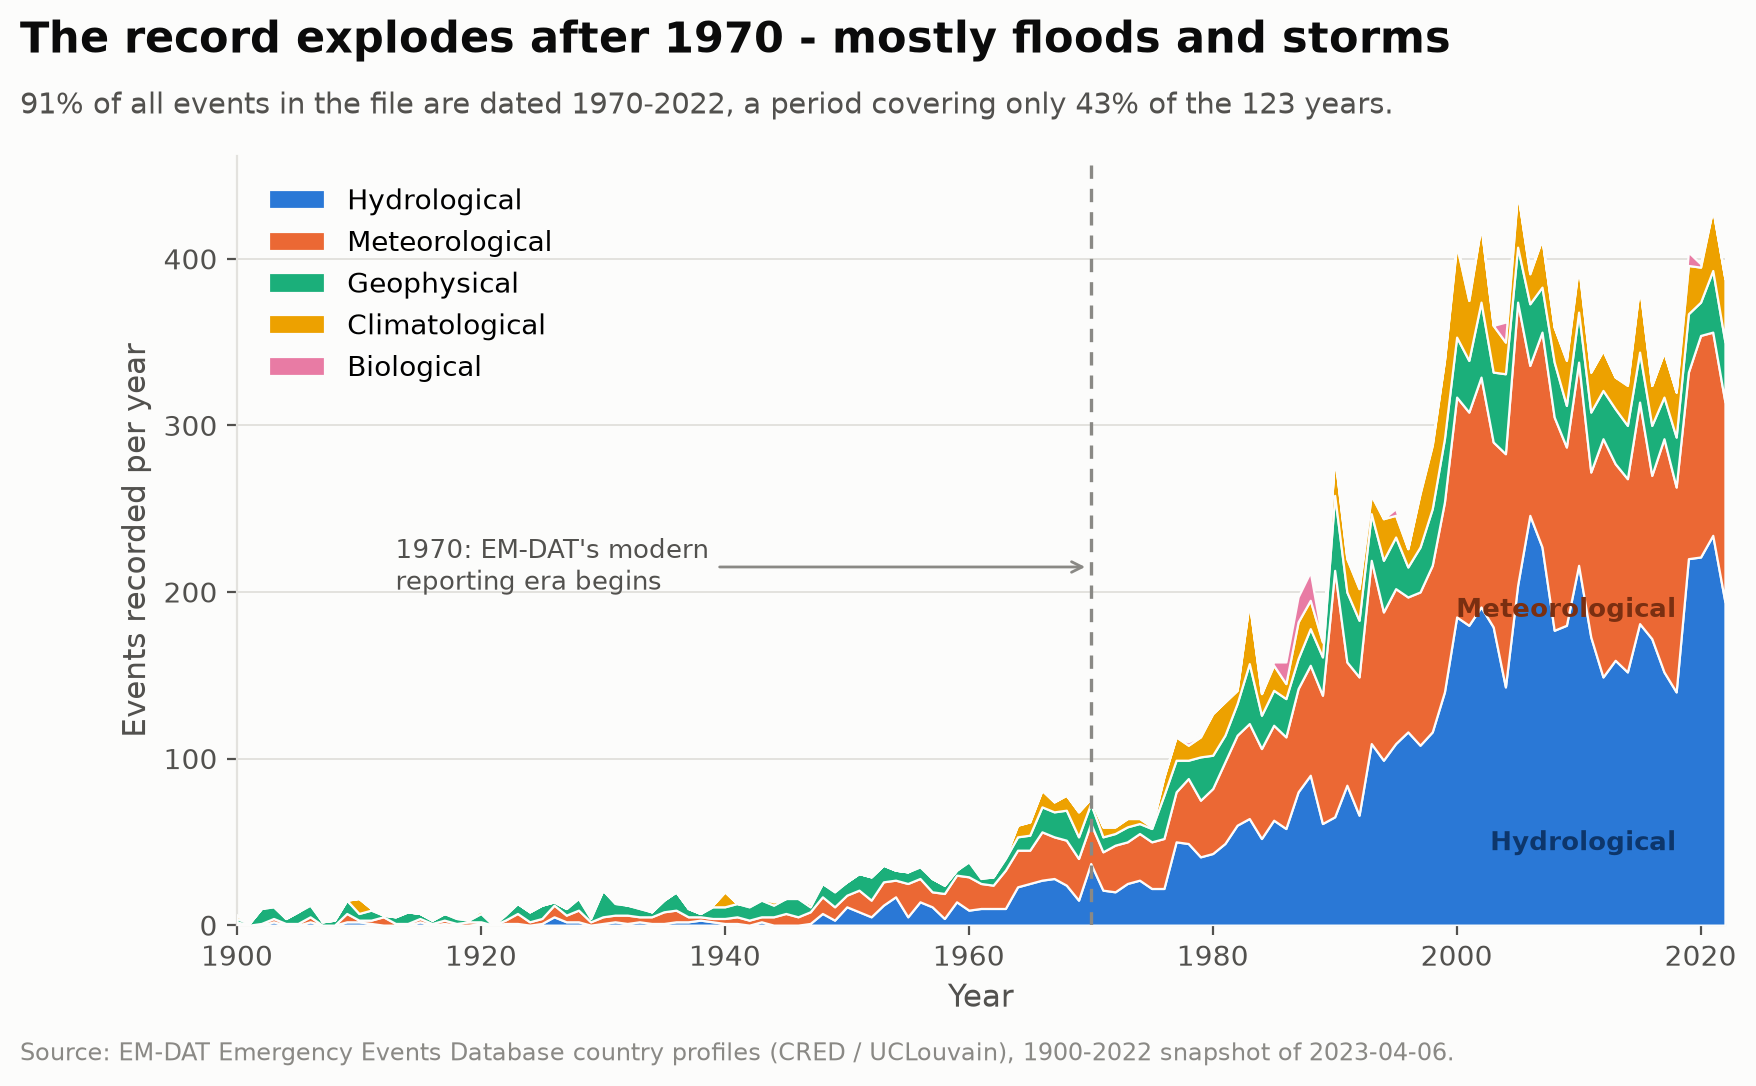
\includegraphics[width=\figw]{Fig4}
\caption[Events recorded per year by sub-group]{\textbf{Events recorded per
year, stacked by disaster sub-group.} A stacked area chart is used because the
question is about both the total and its composition over a continuous time
axis. The two largest bands are labelled directly on the chart in addition to
the legend, so identity never depends on colour alone.}
\label{fig:trend}
\end{figure}

\howto The horizontal axis is the calendar year and the vertical axis is the
number of events recorded in that year. The coloured bands are stacked, so the
height of a band is that sub-group's contribution and the height of the whole
stack is the total for that year. Colour identifies the sub-group: the legend
gives all five, and the two largest bands are also labelled directly on the
chart. The dashed vertical line marks 1970, the point after which EM-DAT's
coverage becomes systematic.

\inference The curve is close to flat until roughly 1960 and then rises steeply,
peaking at 440 events in 2005. The growth is overwhelmingly hydrological and
meteorological --- floods and storms --- which is consistent with a
climate-driven increase, but the shape of this curve is also exactly what a
step-change in data collection would look like. \textbf{91\% of all events in the
file are dated 1970--2022, a span covering only 43\% of the years.} That is a
suspicious concentration, and Figure~\ref{fig:reporting} tests it directly.

\taskhead{A1.3}{Identify: is the rise real, or is it record-keeping?}

\begin{figure}[H]
\centering
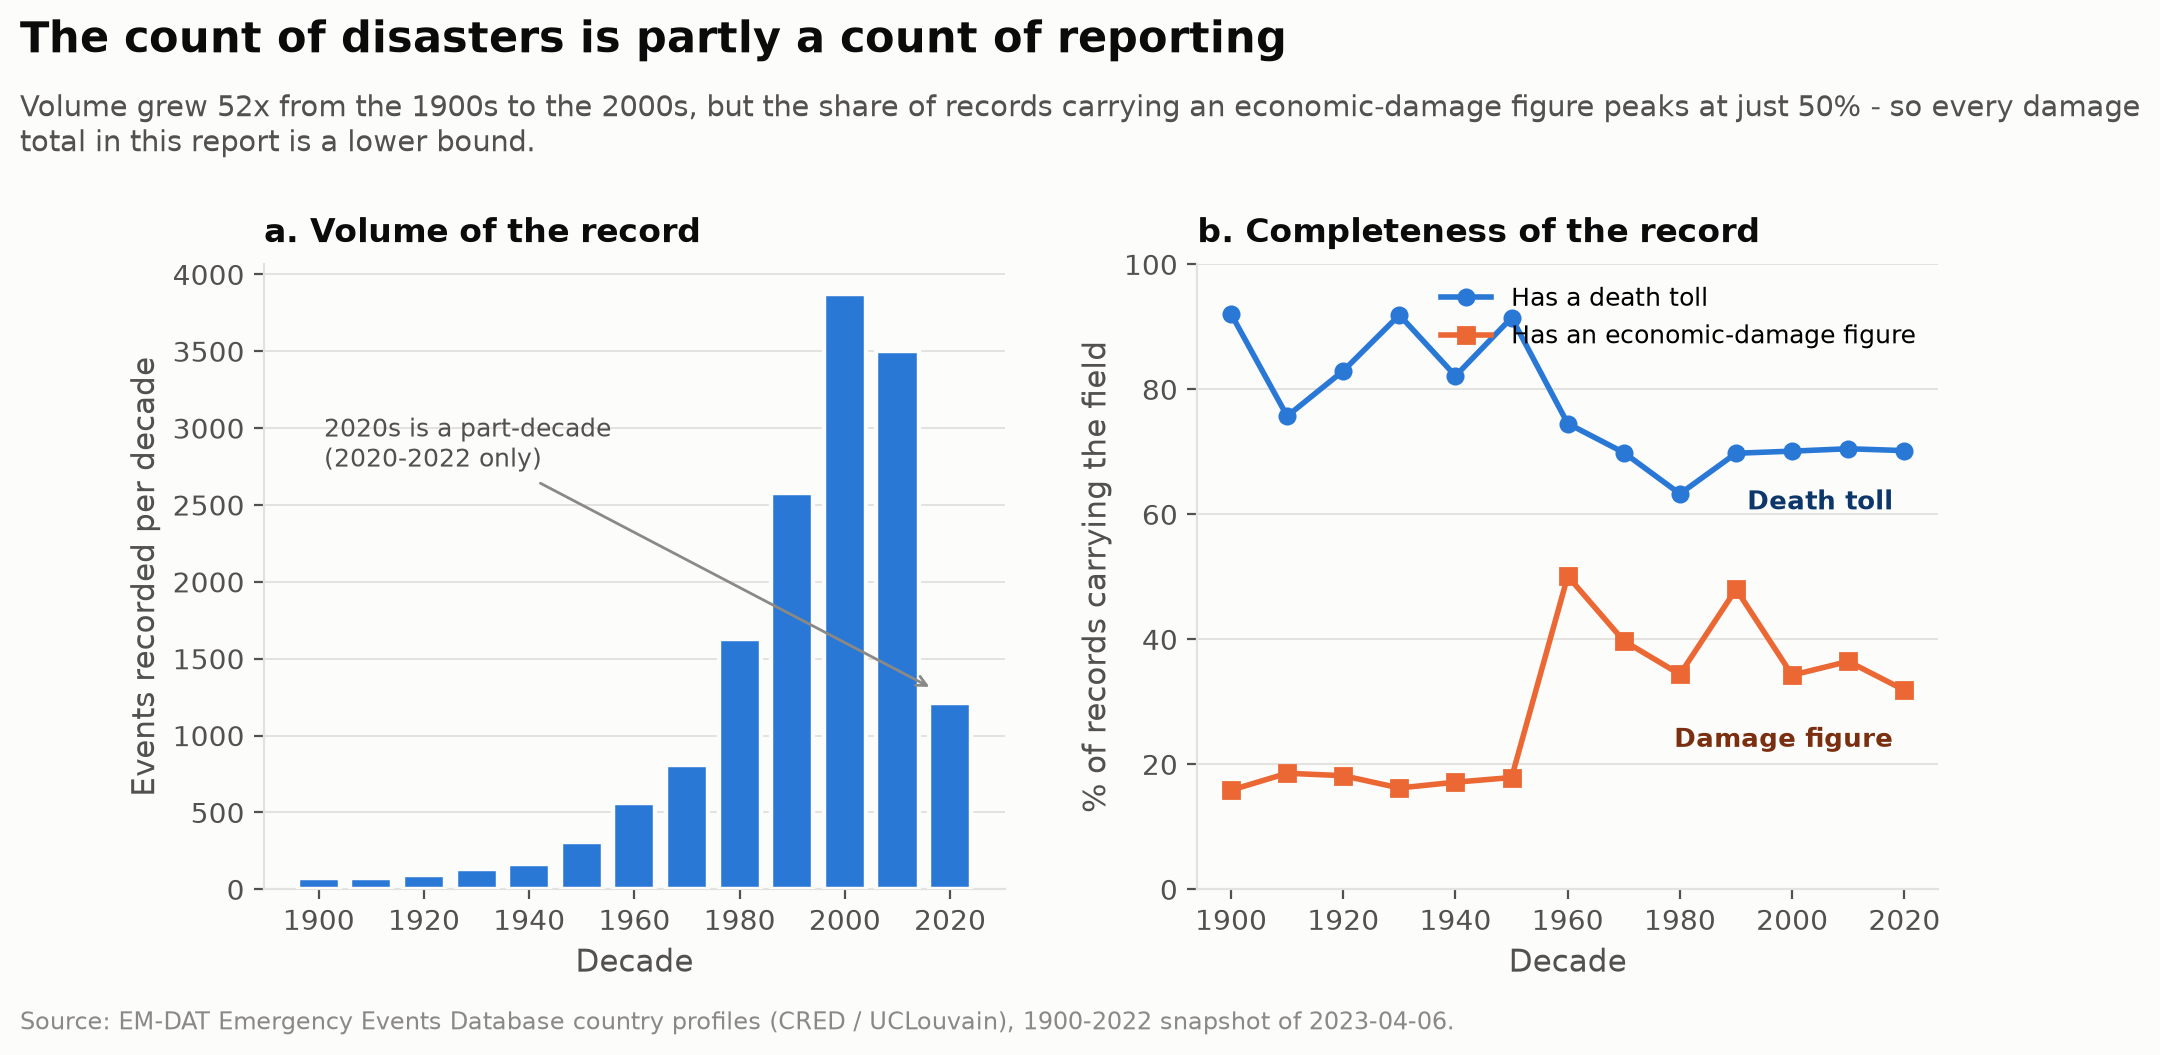
\includegraphics[width=\figw]{Fig5}
\caption[Volume and completeness of the record]{\textbf{Volume and completeness
of the record.} Left: events recorded per decade. Right: the share of records
that actually carry a death toll and a damage figure, by decade. Two panels
rather than one chart, because volume and completeness are different measures;
putting them on a shared $y$-axis would be meaningless.}
\label{fig:reporting}
\end{figure}

\howto Two separate panels, because they measure different things. In panel
(a) the horizontal axis is the decade and the bar height is the number of events
recorded in it --- this is \emph{volume}. In panel (b) the horizontal axis is the
same decade, but the vertical axis is a percentage fixed from 0 to 100: the blue
circles are the share of that decade's records that carry a death toll, and the
orange squares the share that carry an economic-damage figure. Panel (b) is
therefore about \emph{completeness}, not about disasters. Read panel (a) as the
claim and panel (b) as the audit of it.

\rationale This is the diagnostic figure of the report. Before drawing any
conclusion from a rising count, we ask whether the instrument changed.

\inference Recorded volume grew \textbf{52-fold} between the 1900s (74 events)
and the 2000s (3{,}872 events) --- a rate no plausible physical change in hazard
frequency could produce on its own. Meanwhile, the share of records carrying an
economic-damage figure peaks at just 50\% in any decade, and sits between 32\%
and 48\% across the entire post-1970 period. The honest reading is that the event
count in Figure~\ref{fig:trend} is \textbf{a joint measurement of hazard and of
reporting effort, and cannot be separated into the two}. Every subsequent figure
in this report therefore prefers \emph{rates} (deaths per event, share of total,
damage per event) over raw counts, because a rate is far less sensitive to how
many events were catalogued.

\taskhead{A1.4}{Compare: total mortality against mortality per event}

\begin{figure}[H]
\centering
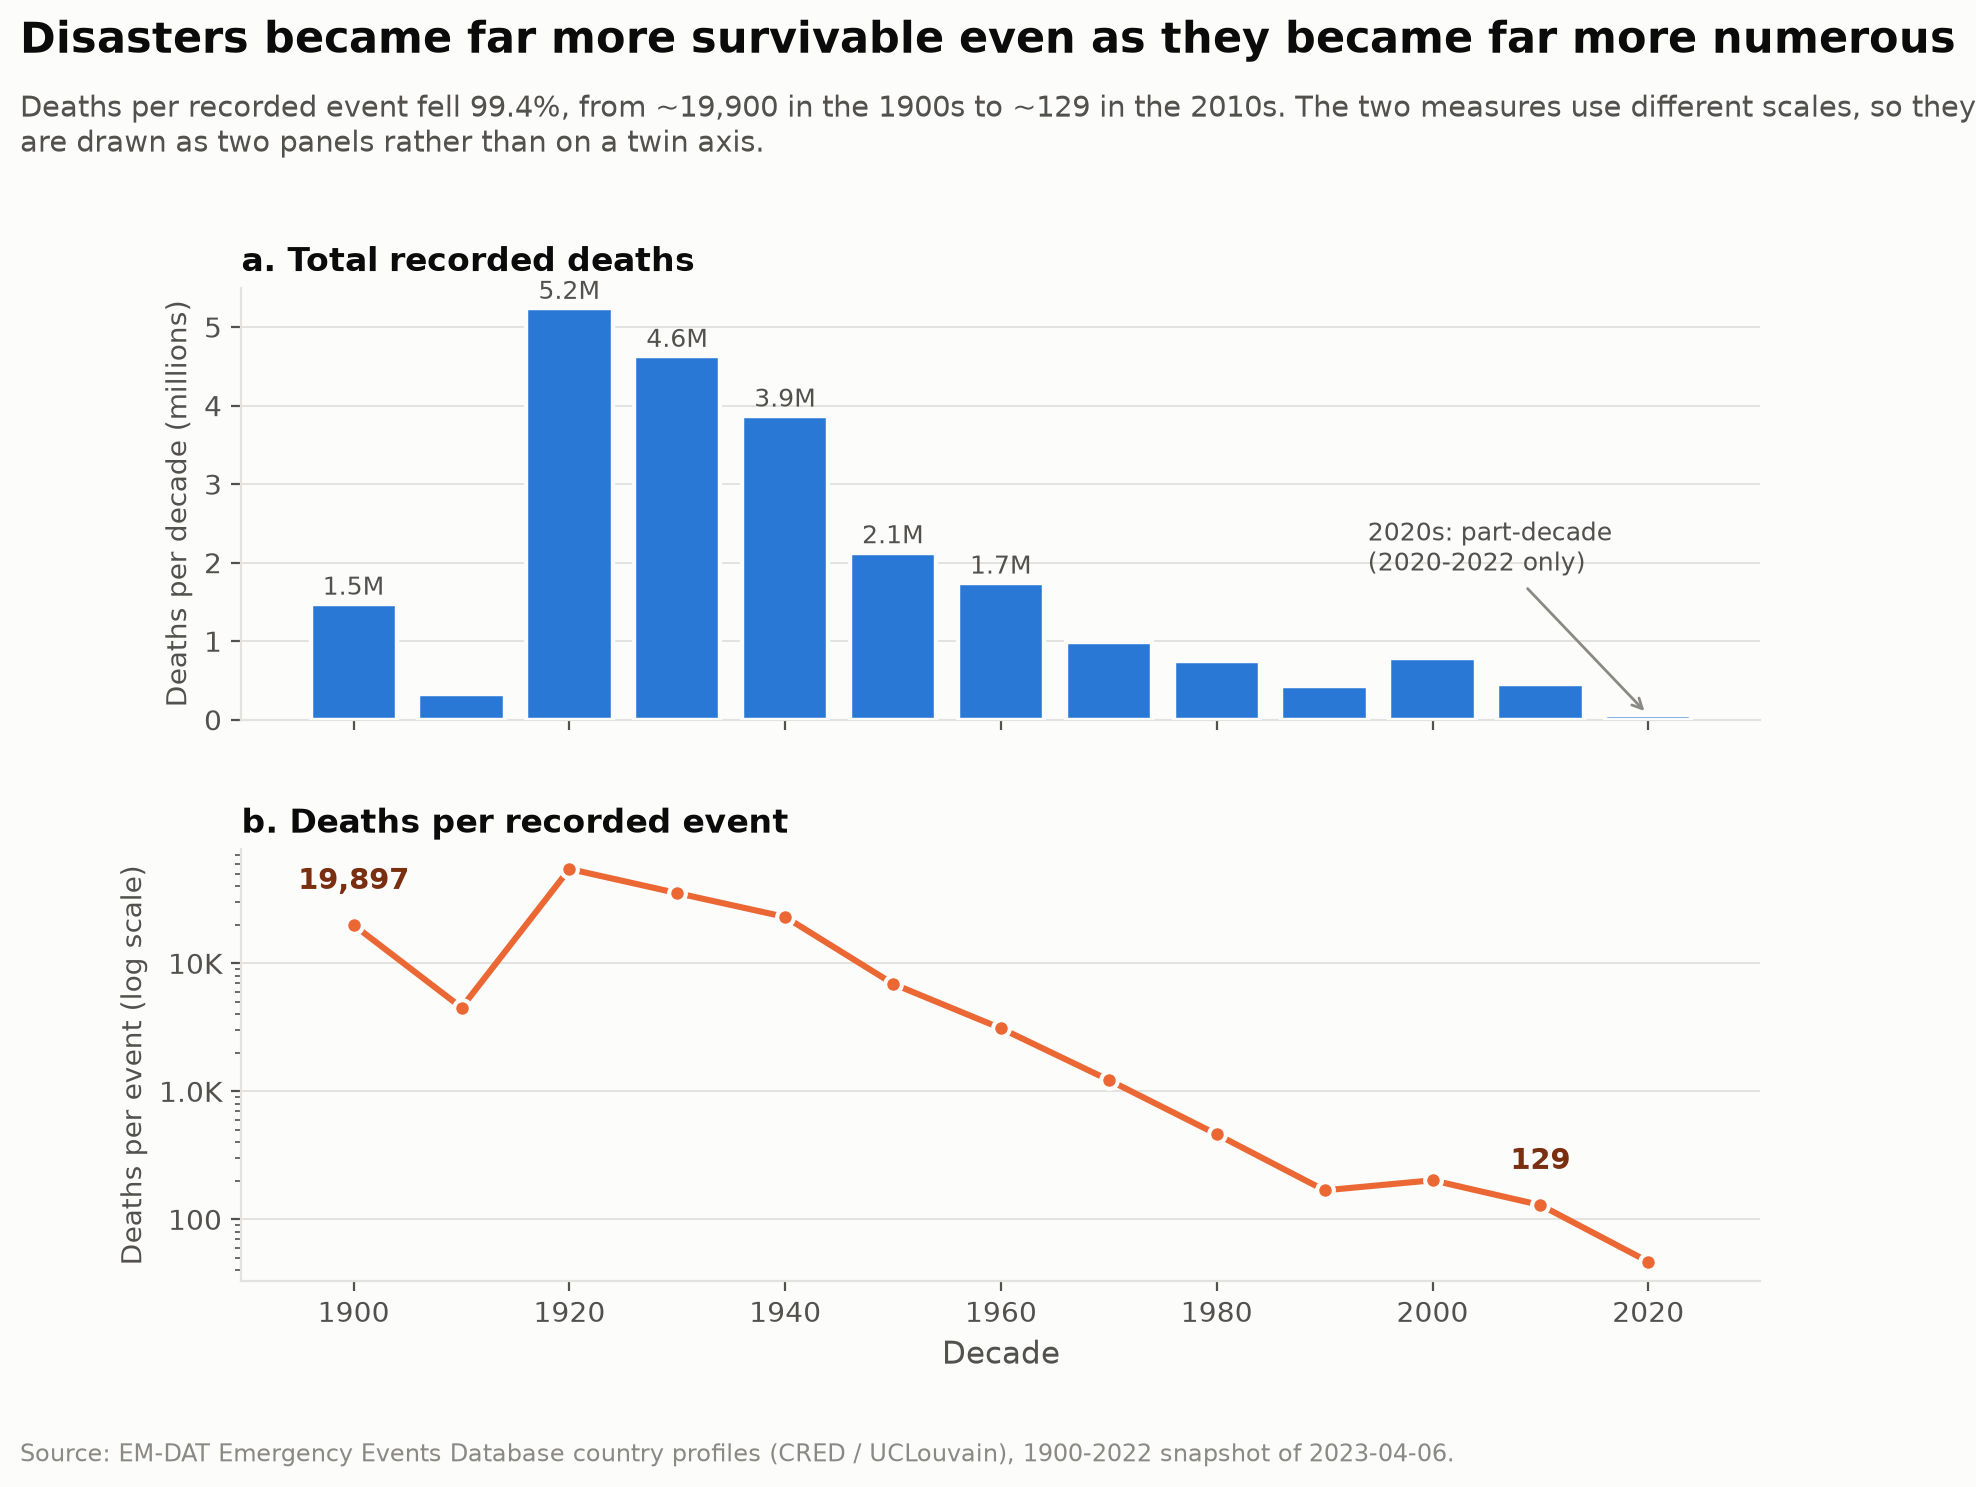
\includegraphics[width=\figw]{Fig6}
\caption[Total deaths versus deaths per event]{\textbf{Total recorded deaths
against deaths per recorded event.} Panel (a) totals deaths by decade; panel (b)
divides by the number of events, on a log scale. The two measures differ by five
orders of magnitude, so they are drawn as two panels sharing one $x$-axis rather
than on a twin $y$-axis.}
\label{fig:deaths}
\end{figure}

\howto Both panels share the same horizontal axis, the decade. Panel (a) is a
bar chart of total recorded deaths in millions, on an ordinary linear scale, with
the taller bars labelled. Panel (b) divides those same deaths by the number of
recorded events, and its vertical axis is \emph{logarithmic}: each labelled
gridline is ten times the one below it, so a straight fall down this axis is a
repeated tenfold reduction, not a fixed one. The two end values are labelled. The
figure is read by comparing the direction of the two panels, which is the whole
point --- (a) falls gently, (b) collapses.

\inference The two panels point in opposite directions, and that contradiction is
the centre of the data story. Total deaths peaked in the \textbf{1920s at 5.24
million} and have fallen to 0.45 million in the 2010s. Deaths per recorded event
fell from \textbf{$\approx$19{,}900 in the 1900s to $\approx$129 in the 2010s ---
a 99.4\% decline}. Whatever has happened to the frequency of disasters, an
individual recorded disaster today kills roughly \textbf{one 150th} of what one
did a century ago. This is the single strongest signal in the dataset.

\taskhead{A1.5}{Validate: is the mortality decline broad-based?}

\begin{figure}[H]
\centering
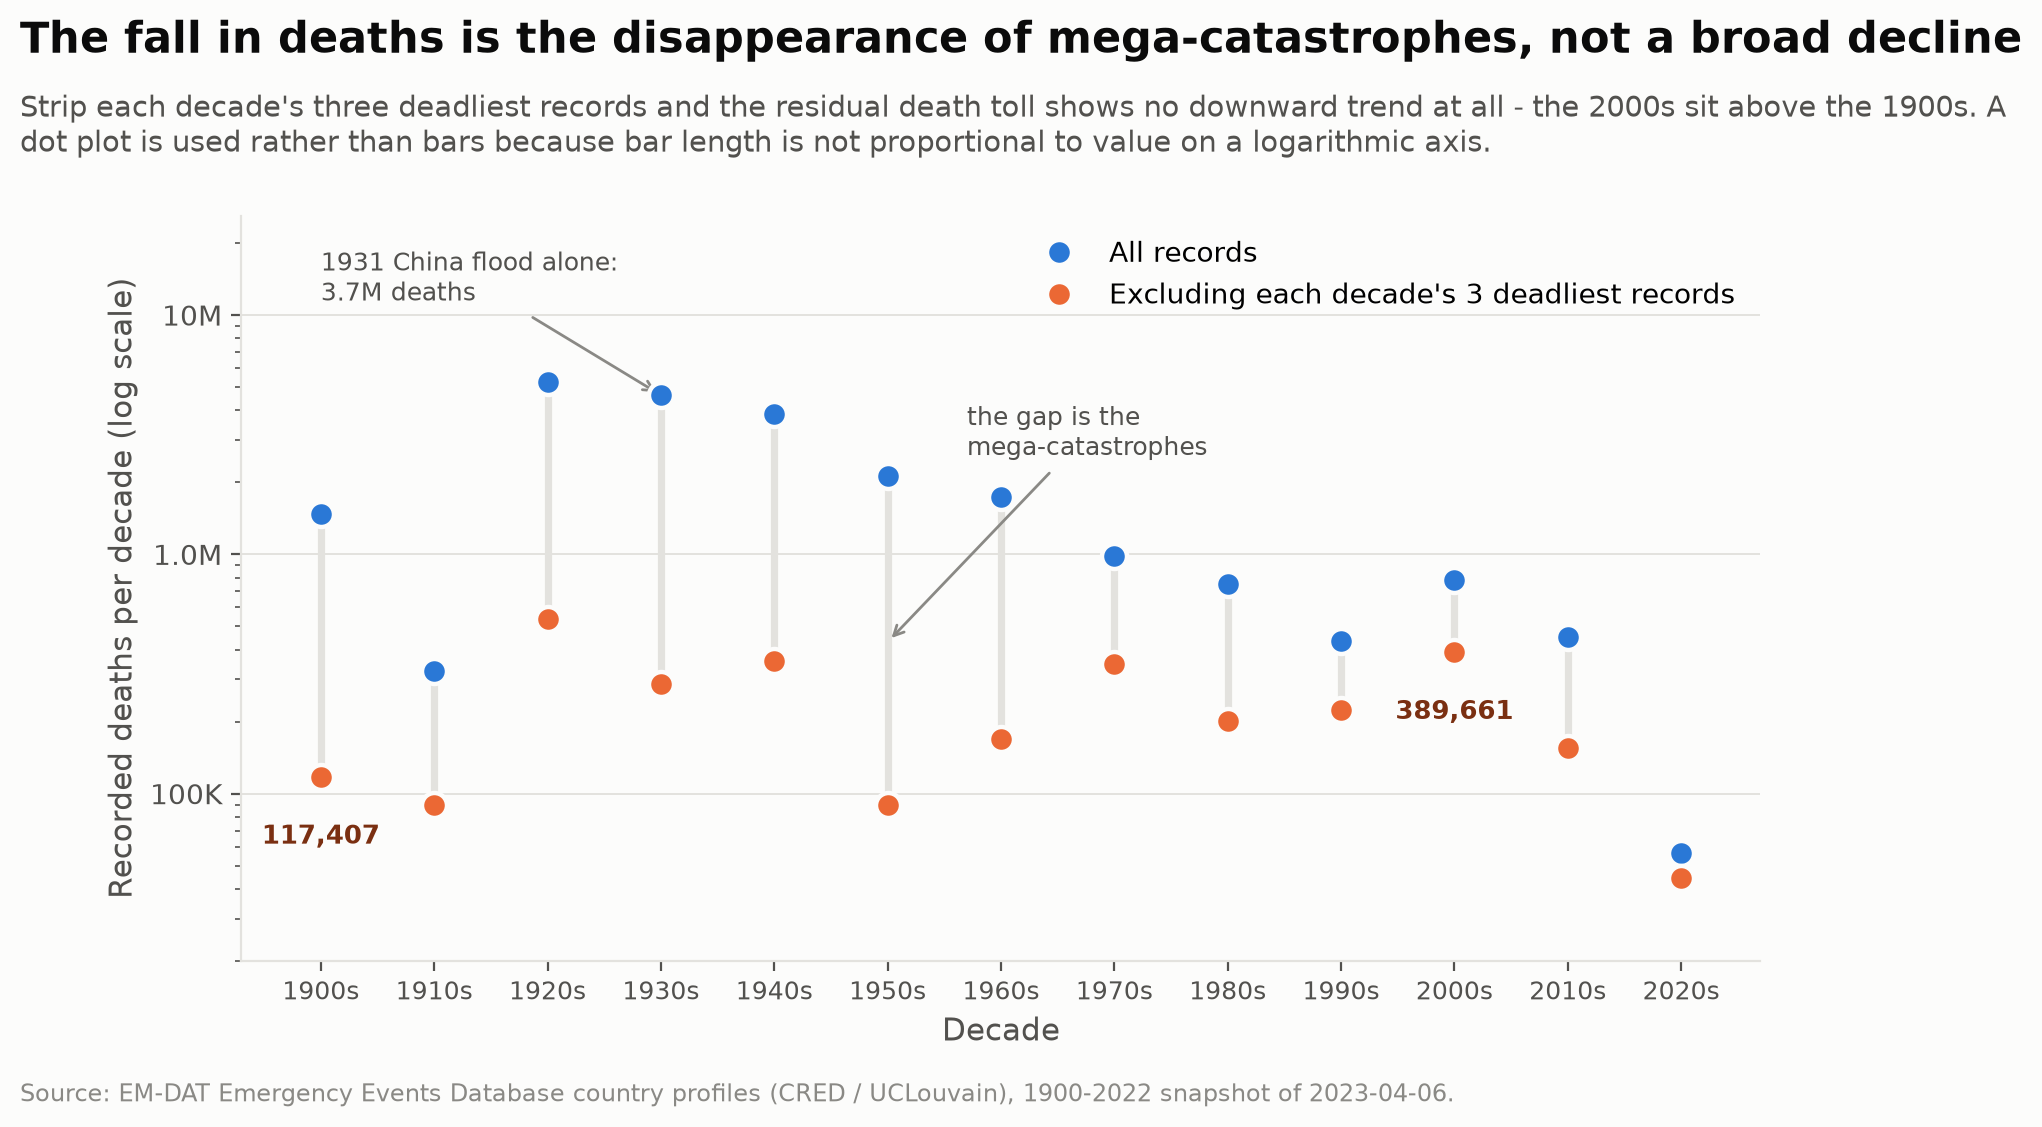
\includegraphics[width=\figw]{Fig7}
\caption[Deaths per decade with and without the deadliest records]{\textbf{Deaths
per decade, with and without each decade's three deadliest records.} A paired dot
plot: each decade has one dot per treatment and a connector whose length is the
contribution of the three deadliest records. A log scale is required because the
values span three orders of magnitude --- and that is precisely why dots are used
rather than bars, since bar \emph{length} is not proportional to value once the
axis is logarithmic, whereas dot \emph{position} still is. This figure is a
deliberate attempt to break the result of Figure~\ref{fig:deaths}.}
\label{fig:trimmed}
\end{figure}

\howto Each decade has two dots. The blue dot is that decade's total recorded
deaths; the orange dot is the same total after the three single deadliest records
of that decade are removed. The grey bar joining them is therefore not a bar in
the usual sense --- its length \emph{is} the amount contributed by just those
three records. The vertical axis is logarithmic, so equal vertical distances are
equal ratios. Read the chart by ignoring the dots for a moment and looking only
at the connectors: they are long on the left and short on the right, which says
the early decades were dominated by a handful of enormous events.

\rationale A 99.4\% fall is a large claim. Because EM-DAT's early decades are
dominated by a handful of enormous famines and floods, we test whether the
decline survives their removal.

\inference \textbf{It does not, in the form usually stated.} Once each decade's
three deadliest records are removed, the residual death toll shows \textbf{no
downward trend whatsoever}: the 2000s (390{,}000) sit \emph{above} the 1900s
(117{,}000). The century-scale collapse in total mortality is almost entirely
\textbf{the disappearance of mega-catastrophes} --- single events such as the
1931 China flood (3.7 million deaths) and the 1928 China drought (3.0 million)
--- rather than a broad reduction in ordinary disaster deaths. This is a
genuinely different conclusion from the headline one, and it is the kind of
finding that only emerges from deliberately trying to break your own result.

%=======================================================================
\section{Task Set B --- \emph{Where?} The Geography of Exposure}
\label{sec:taskB}
%=======================================================================

\textbf{Owner:} \memberB \quad$\cdot$\quad
\textbf{Figures:} \ref{fig:mapevents}--\ref{fig:lethality} \quad$\cdot$\quad
\textbf{Script:} \texttt{code/task\_b\_geography.py}

\taskhead{B1.1}{Locate: where are disasters recorded?}

\begin{figure}[H]
\centering
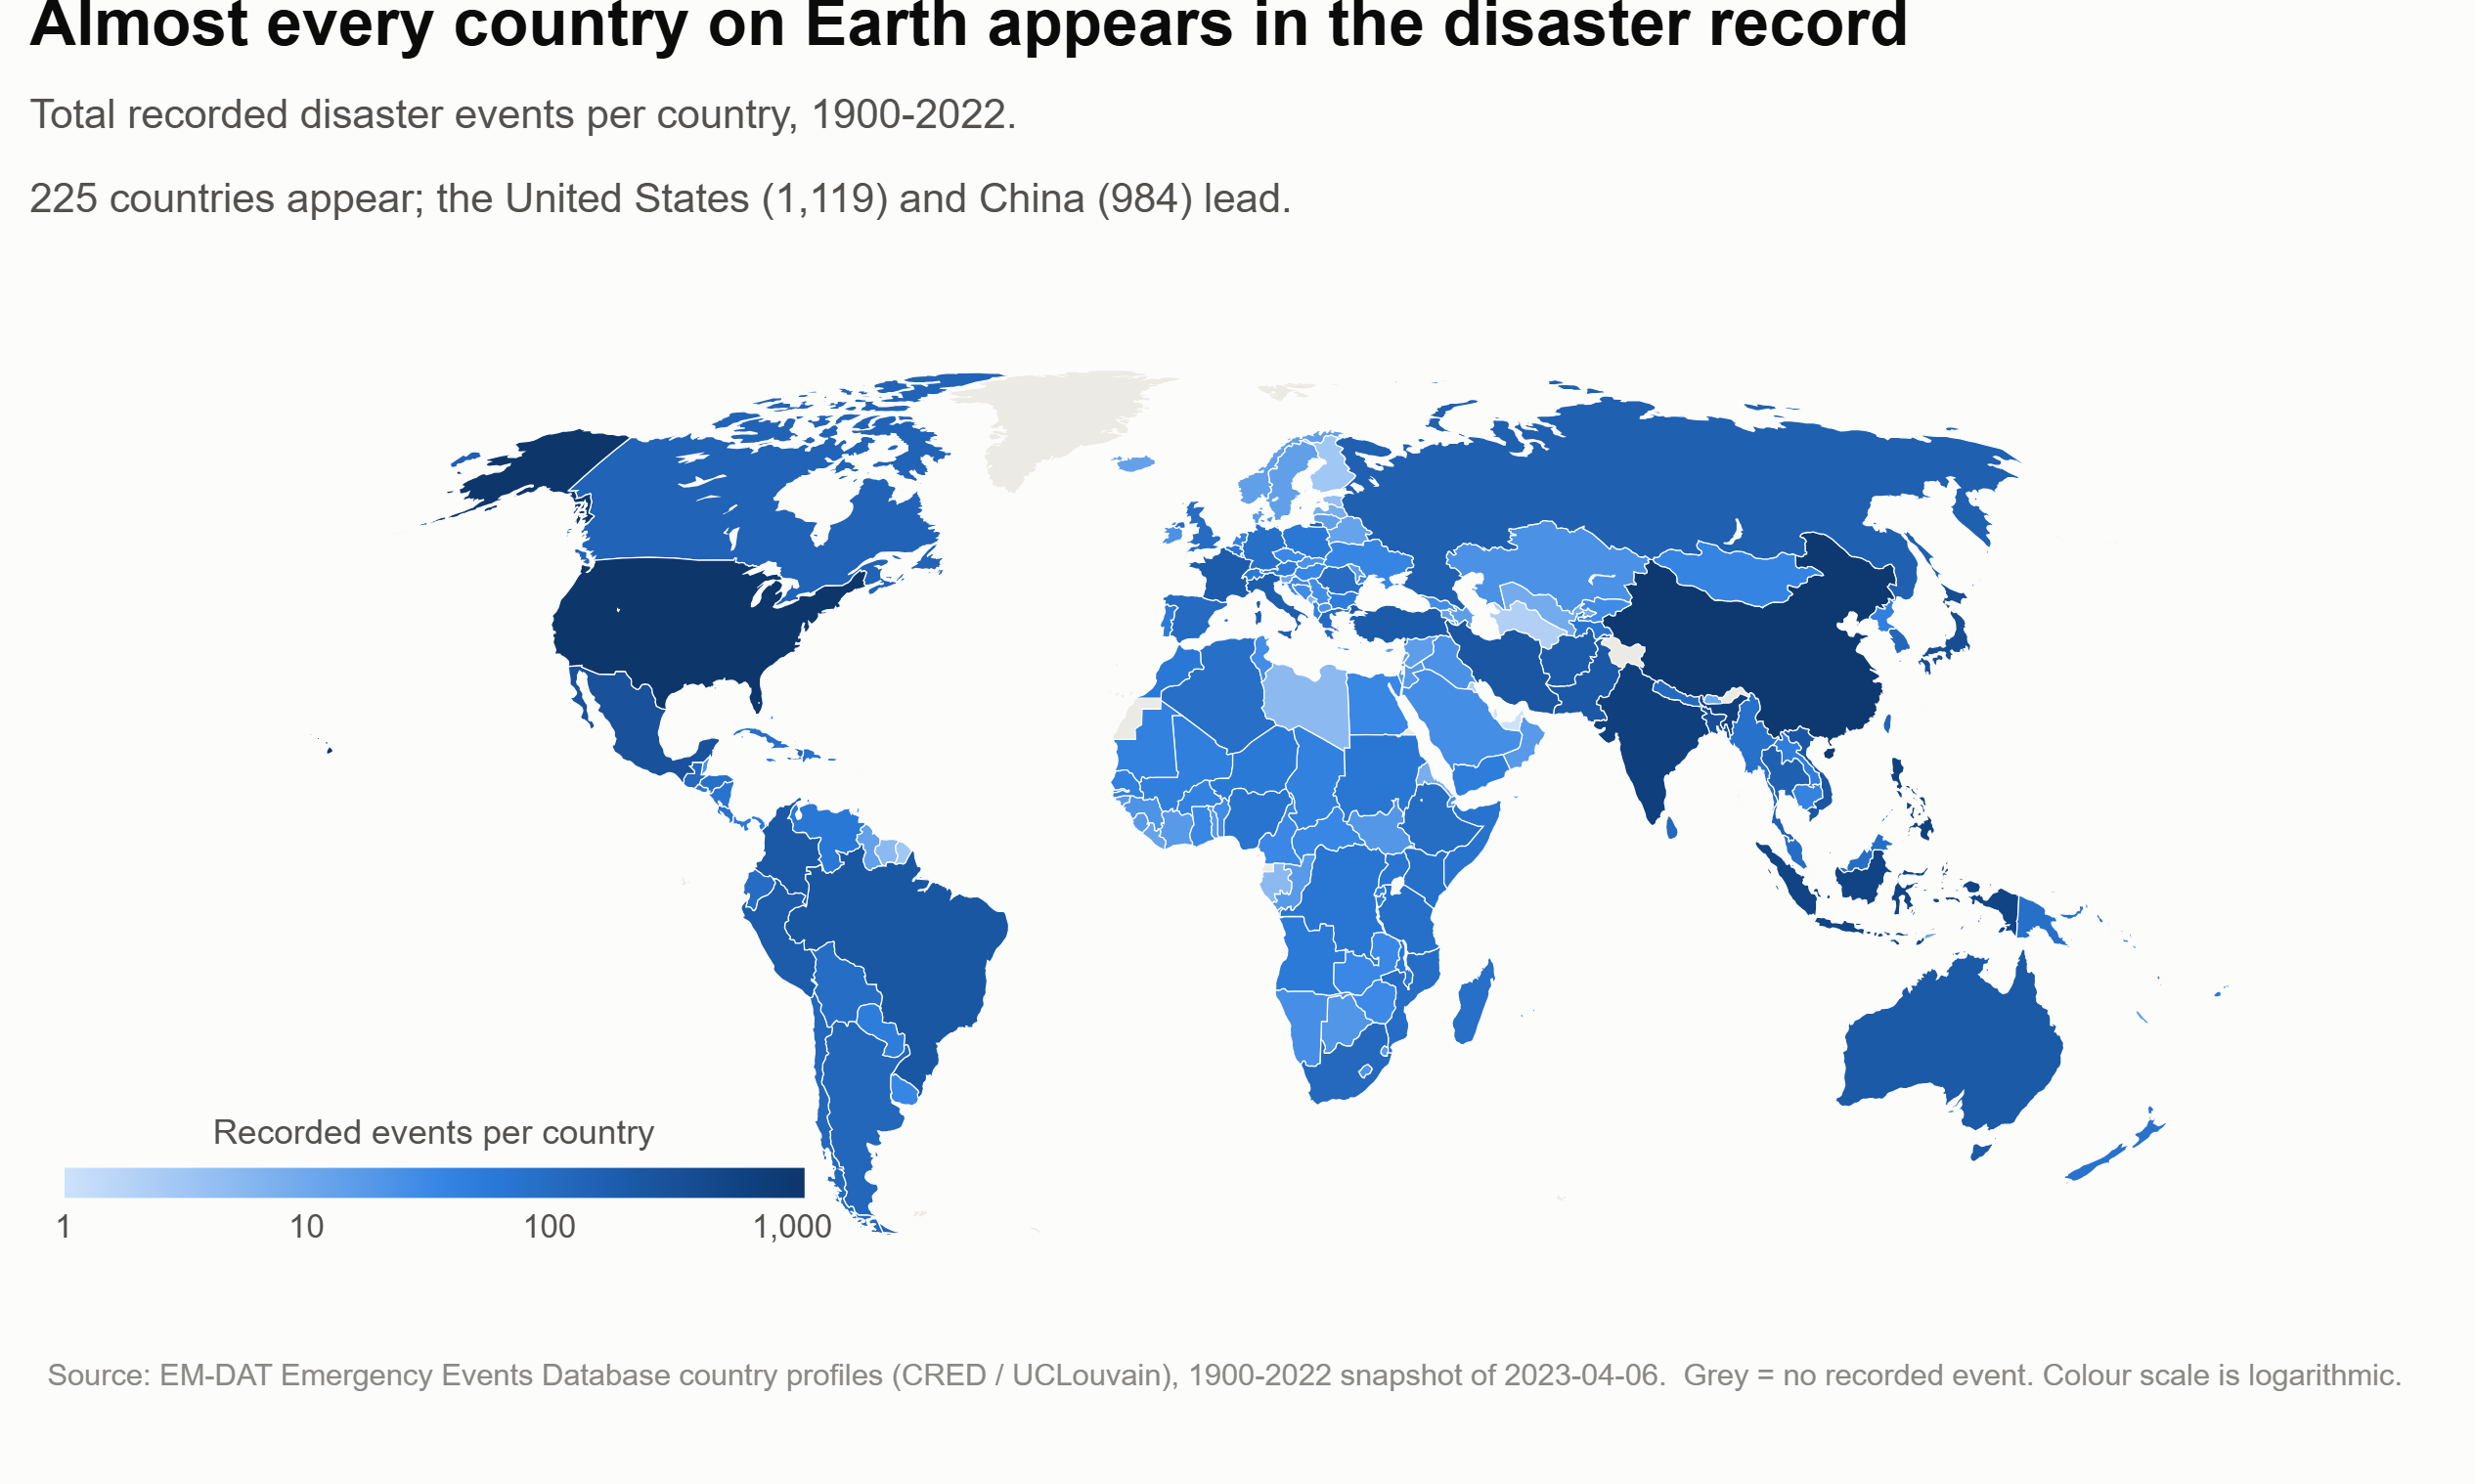
\includegraphics[width=\figw]{Fig8}
\caption[World map of recorded events]{\textbf{Total recorded disaster events per
country, 1900--2022.} A choropleth answers ``where'' directly. The colour scale
is a single-hue sequential blue ramp on a \emph{logarithmic} scale --- country
totals span five orders of magnitude, and a linear ramp would render every
country except the United States and China identically pale.}
\label{fig:mapevents}
\end{figure}

\howto Every country is filled according to one number: the total count of
disaster events recorded there across 1900--2022. A single blue hue is used, pale
for few and dark for many, so the eye reads only intensity and never has to
decode separate colours. The scale bar beneath the map is \emph{logarithmic} ---
each labelled step (1, 10, 100, 1{,}000) is ten times the previous one, so a
country twice as dark has far more than twice as many events. Grey means no
recorded event at all.

\inference Disaster occurrence is close to universal: all \textbf{225} countries
and territories in the file appear at least once. The darkest countries are the
large, populous, well-documented ones --- the United States (1{,}119 events),
China (984), India (688), the Philippines (659) and Indonesia (570). Note that
this map is as much a map of \emph{area, population and reporting capacity} as of
hazard.

\taskhead{B1.2}{Locate: where do people actually die?}

\begin{figure}[H]
\centering
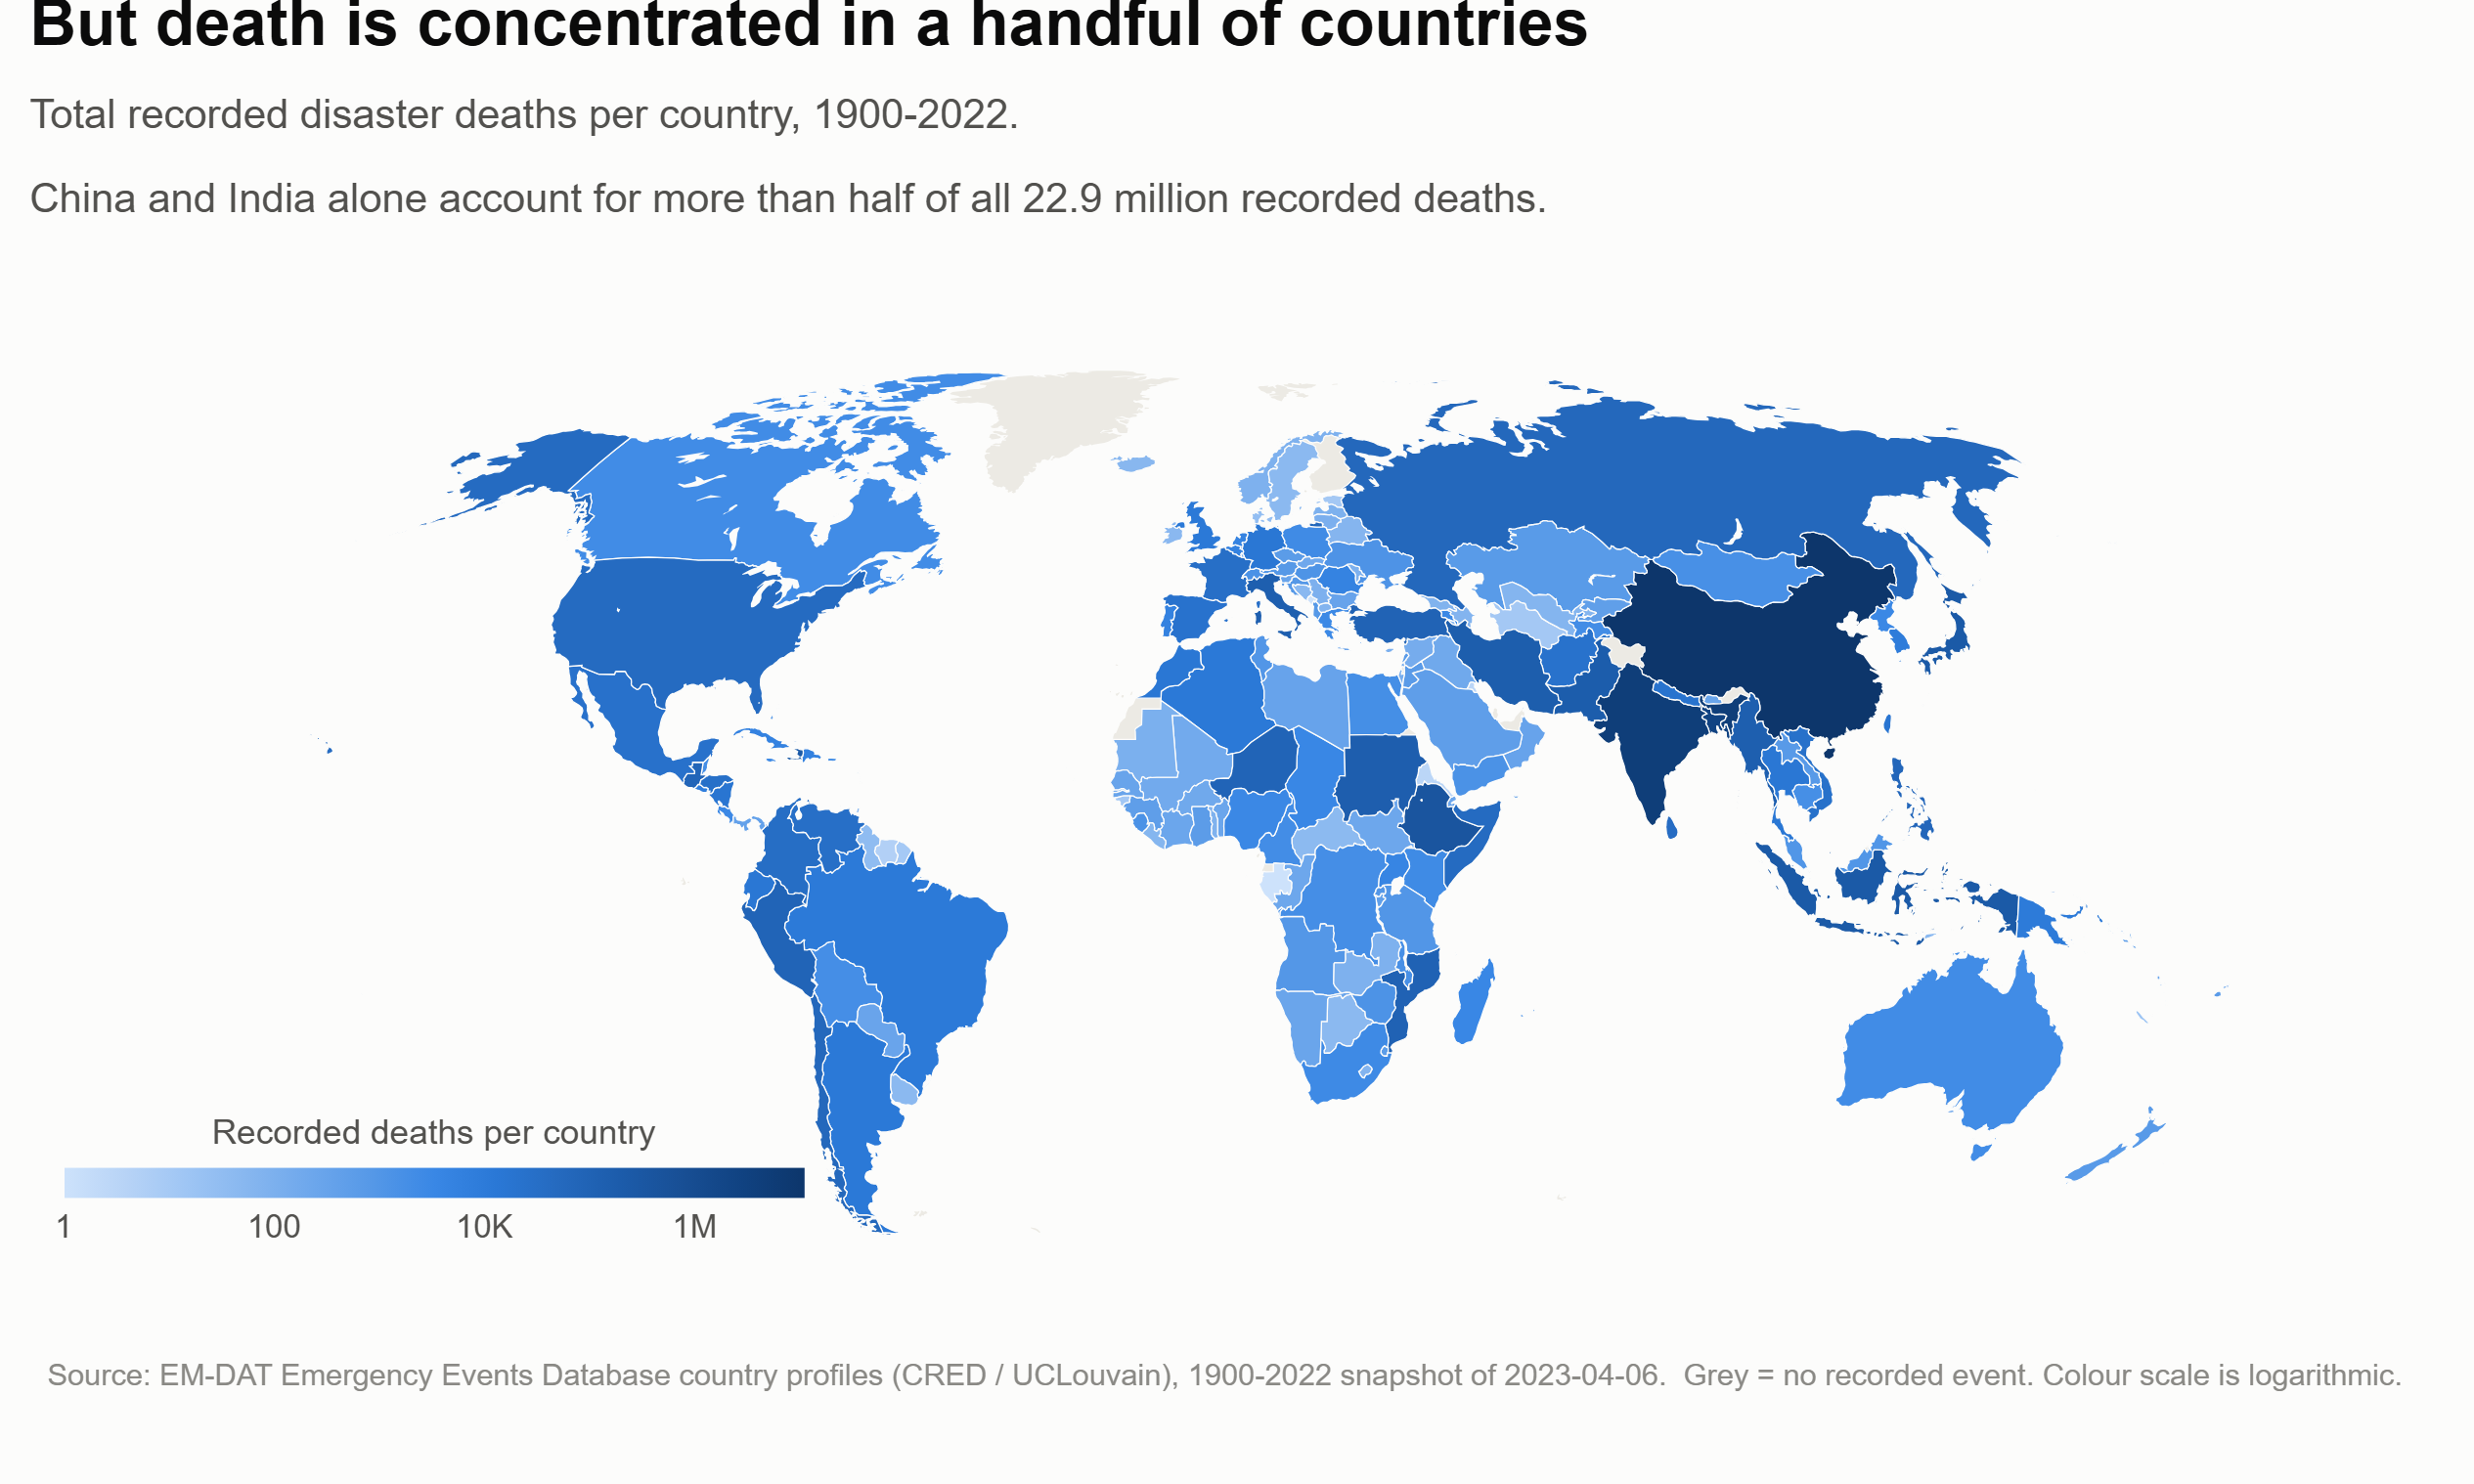
\includegraphics[width=\figw]{Fig9}
\caption[World map of recorded deaths]{\textbf{Total recorded disaster deaths per
country, 1900--2022.} Drawn on the same projection and the same style of
logarithmic colour scale as Figure~\ref{fig:mapevents}, so the two maps can be
read directly against each other. Holding the encoding constant is what makes
the comparison legible.}
\label{fig:mapdeaths}
\end{figure}

\howto Identical in construction to Figure~\ref{fig:mapevents} --- same
projection, same single-hue blue ramp, same logarithmic scale --- but the number
driving the fill is now total recorded deaths rather than event count. Holding
everything except the measure constant is deliberate: any difference you see
between the two maps is a difference in the data, not in how it was drawn.

\inference The map changes character completely. Where
Figure~\ref{fig:mapevents} is broadly shaded, Figure~\ref{fig:mapdeaths} is
dominated by two countries. \textbf{China (10.96 million) and India (4.59
million) alone account for 68\% of all 22.86 million recorded deaths};
Bangladesh adds a further 2.59 million. The United States, which leads the world
in \emph{recorded events}, ranks \textbf{23rd} in deaths with 44{,}246.
Occurrence and mortality are not the same geography.

\taskhead{B1.3}{Rank: four burdens, four leaderboards}

\begin{figure}[H]
\centering
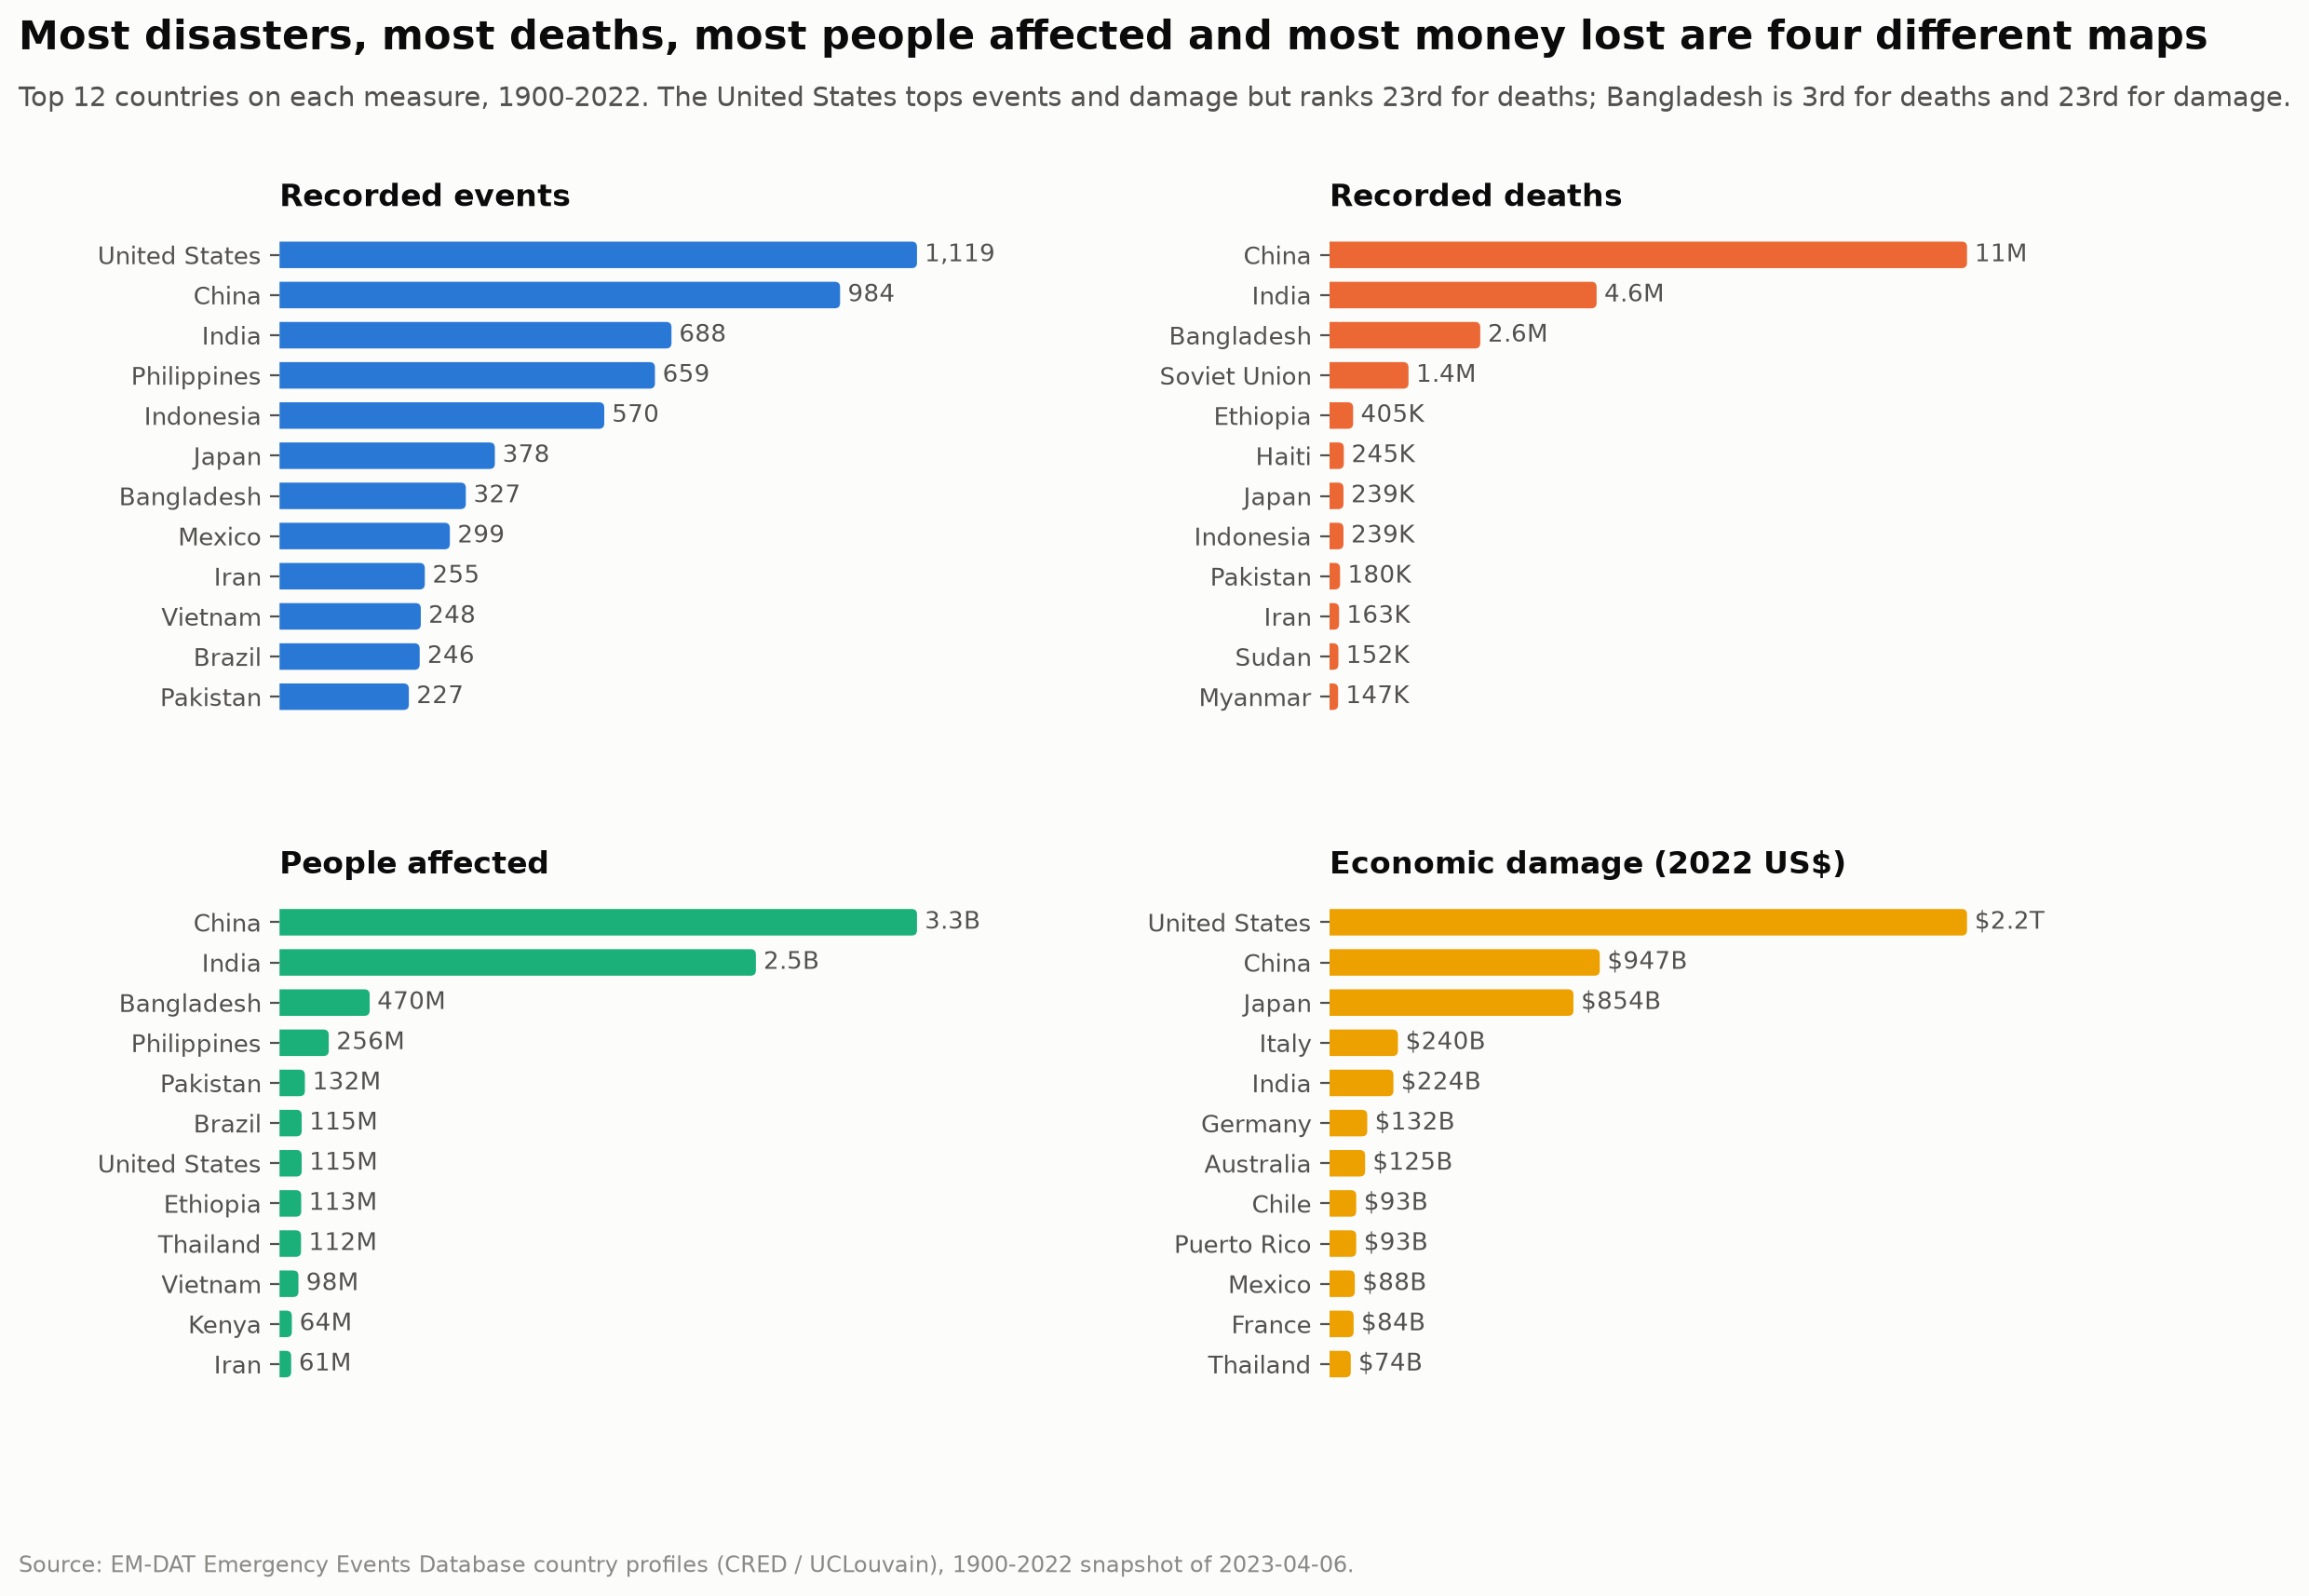
\includegraphics[width=\figw]{Fig10}
\caption[Top countries on four measures]{\textbf{Top 12 countries on each of four
measures.} Small multiples of ranked bars, each panel on its own scale, because
the question is rank \emph{within} a measure rather than magnitude \emph{across}
measures. Every bar is directly labelled with its value, so no reading off an
axis is required.}
\label{fig:leaderboards}
\end{figure}

\howto Four separate rankings, one per panel. Within a panel, the twelve
longest bars are the twelve highest-ranking countries on that measure, longest at
the top, and every bar carries its own value label. Each panel has its own
horizontal scale and no axis is drawn, so bar lengths should be compared
\emph{within} a panel and never across panels --- the comparison this figure
invites is of the \emph{membership and order} of the four lists, not of their
magnitudes.

\inference The four leaderboards barely overlap, and the mismatches are the
finding:

\begin{itemize}
\item The \textbf{United States} is 1st for events and 1st for damage (\$2.23
  trillion) but \textbf{23rd} for deaths.
\item \textbf{Bangladesh} is \textbf{3rd} for deaths (2.59 million) but
  \textbf{23rd} for damage.
\item \textbf{Australia} is 14th for events and \textbf{7th} for damage but
  \textbf{69th} for deaths.
\item \textbf{Japan} is 3rd for damage (\$854 billion) but 31st for people
  affected.
\end{itemize}

Wealth appears to convert disaster exposure into property loss rather than into
death. The Soviet Union appears 4th for deaths --- a reminder that the country
field contains historical states (Section~\ref{sec:prep}, rule 7).

\taskhead{B1.4}{Derive: how concentrated is each burden?}

\begin{figure}[H]
\centering
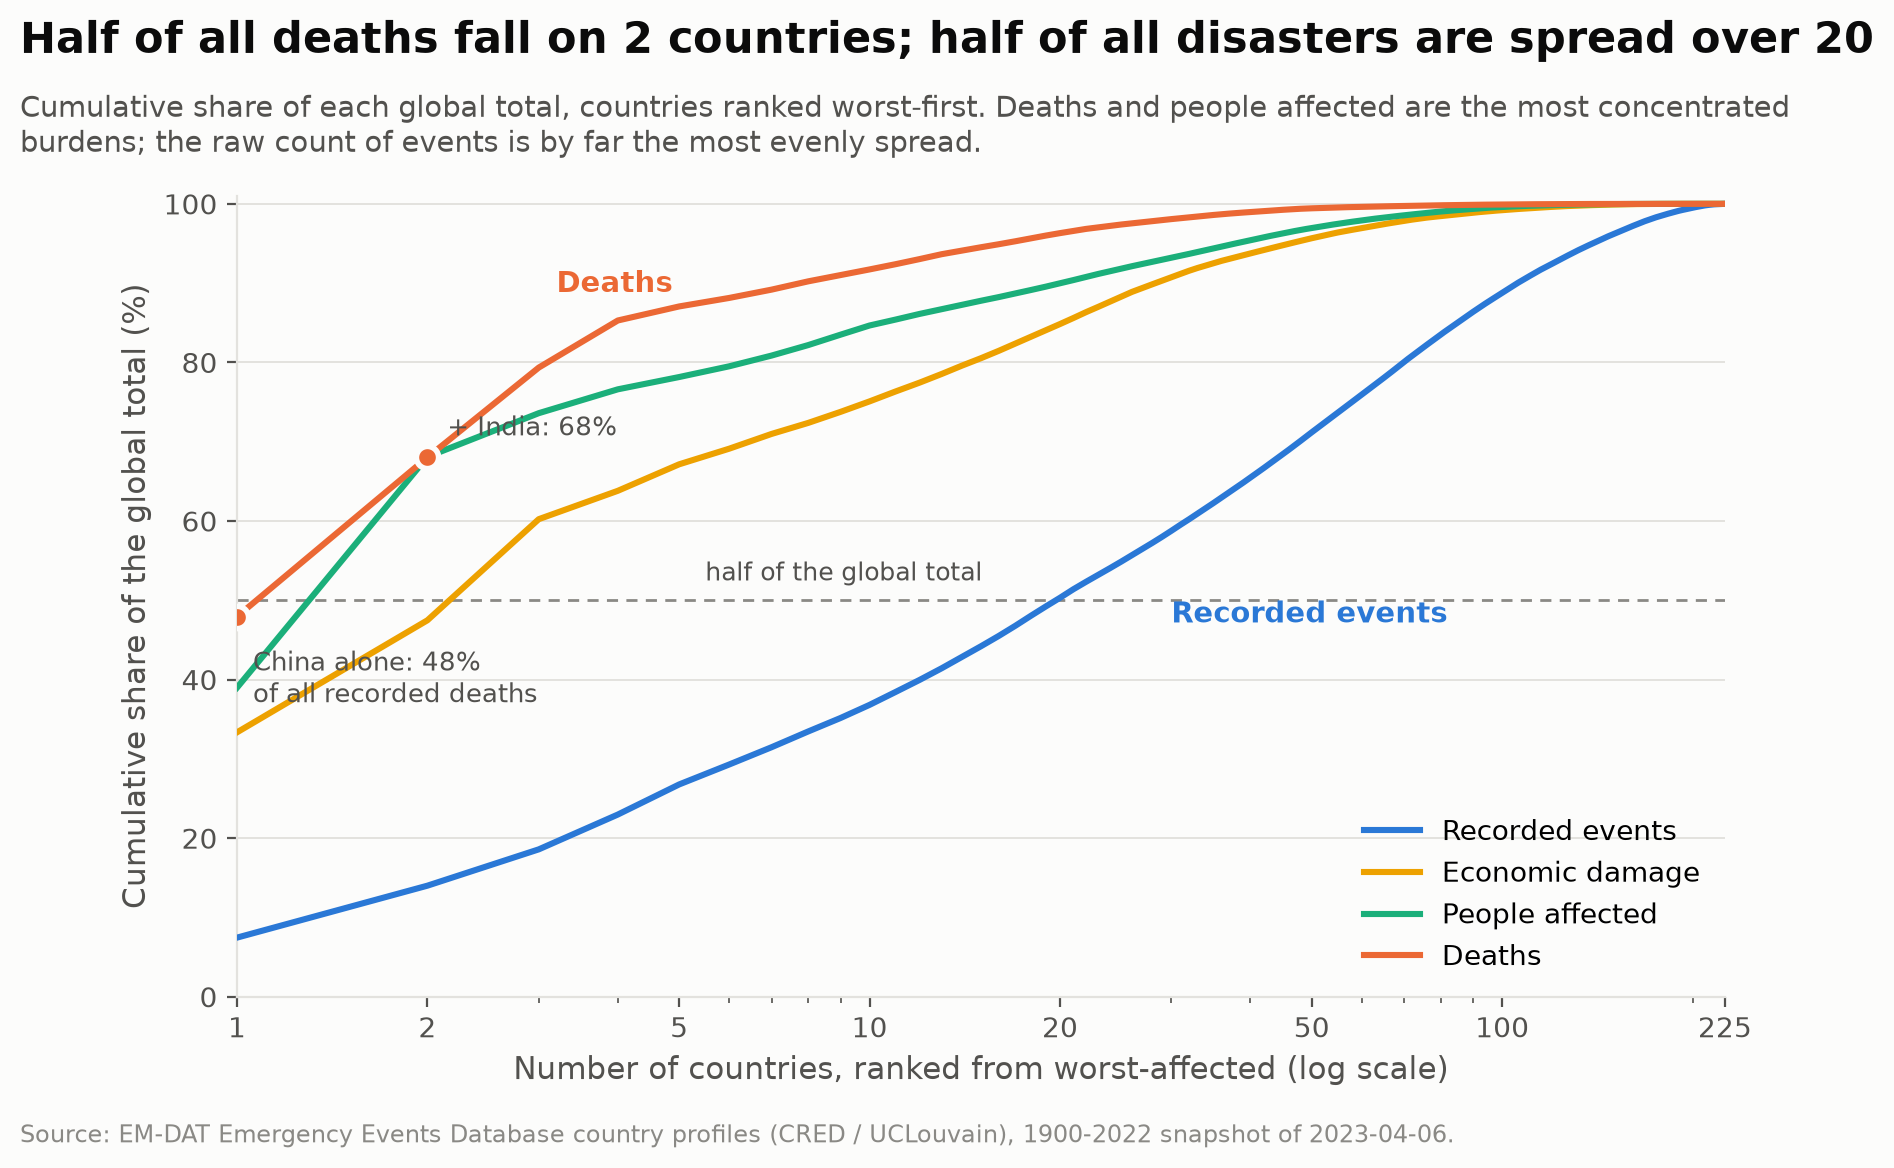
\includegraphics[width=\figw]{Fig11}
\caption[Concentration curves for four burdens]{\textbf{Cumulative share of each
global total against the number of countries}, ranked worst-first, on a
logarithmic $x$-axis. This is a concentration (Lorenz-style) curve: the faster a
curve rises, the fewer countries carry that burden.}
\label{fig:concentration}
\end{figure}

\howto Countries are ranked worst-first for each measure, then accumulated.
A point at $(x, y)$ reads: ``the $x$ worst-affected countries together account
for $y$ per cent of the world total.'' Every curve therefore starts low, rises,
and must end at 100\% once all 225 countries are included. The steeper a curve
rises at the left, the more concentrated that burden is in a few countries. The
horizontal axis is logarithmic so the first handful of countries is legible. The
dashed line marks the 50\% level, and the two dots on the deaths curve mark China
alone and China plus India.

\inference The burdens are concentrated to very different degrees. It takes just
\textbf{2 countries} to pass half of all recorded deaths (China alone is 48\%),
but \textbf{20 countries} to pass half of all recorded \emph{events}. The top
five countries hold \textbf{87.1\%} of deaths, \textbf{78.2\%} of people
affected and \textbf{67.2\%} of damage --- but only \textbf{26.8\%} of events.
Disasters happen nearly everywhere; dying from them does not.

\taskhead{B1.5}{Derive: lethality among comparably exposed countries}

\begin{figure}[H]
\centering
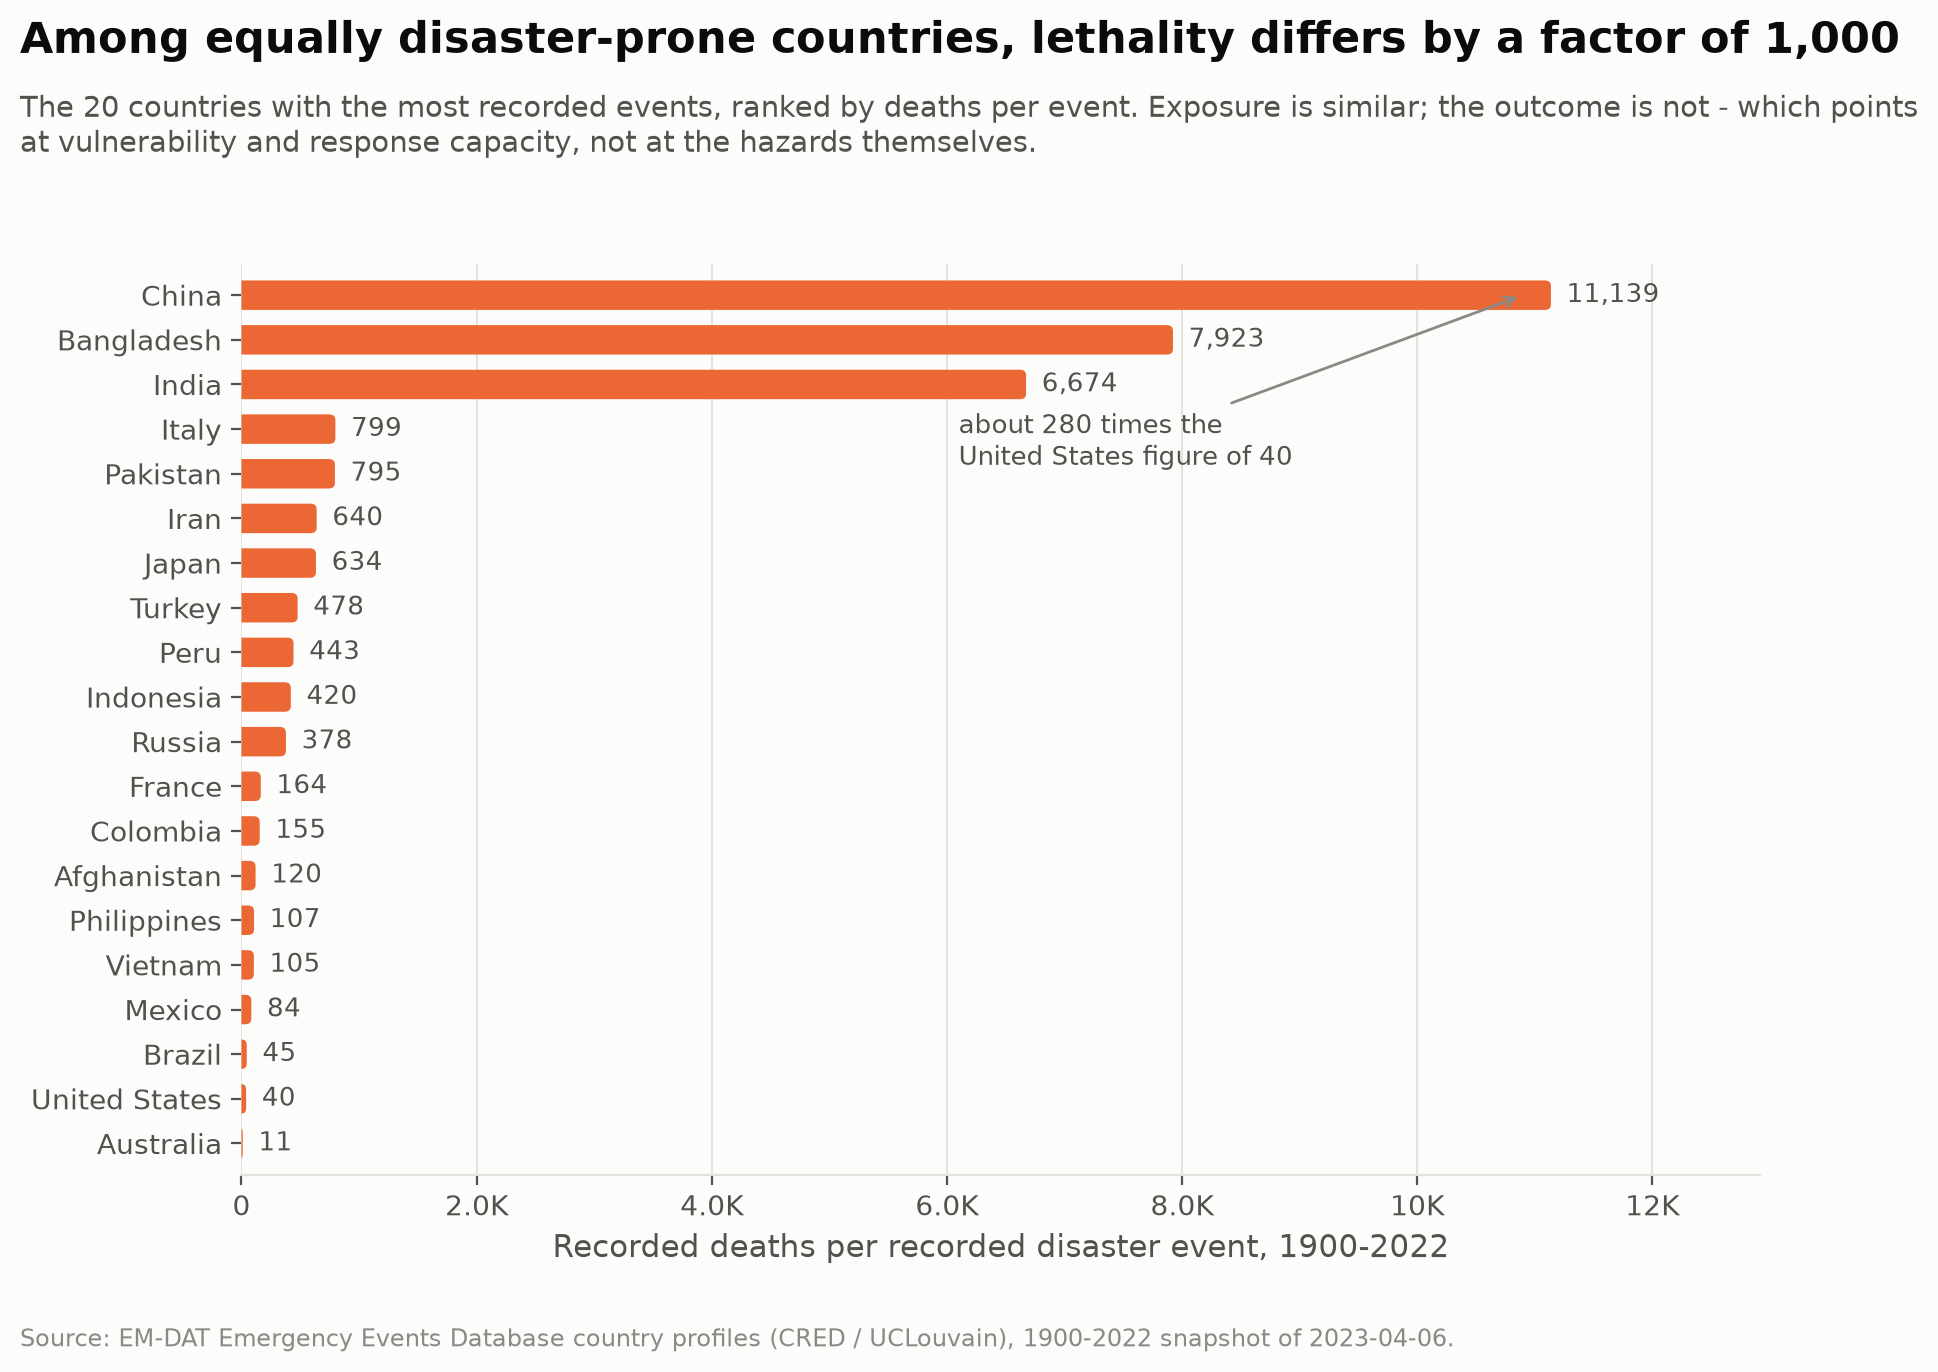
\includegraphics[width=\figw]{Fig12}
\caption[Deaths per event for the most-exposed countries]{\textbf{Deaths per
recorded event for the 20 countries with the most recorded events.} Restricting
to the most disaster-prone countries holds exposure roughly constant, so that the
remaining variation reflects vulnerability rather than hazard frequency.}
\label{fig:lethality}
\end{figure}

\howto Only the 20 countries with the most recorded events appear, which is
what makes the comparison fair: every country shown is heavily disaster-exposed,
so exposure is roughly held constant and the differences are differences in
outcome. Bar length is deaths divided by recorded events --- an average severity,
not a total --- and countries are sorted from the highest to the lowest. Every
bar is labelled, and the axis is linear, so length is directly proportional to
value.

\inference Among countries with broadly comparable exposure, lethality varies by
a factor of about \textbf{1{,}000} --- from China at 11{,}139 deaths per event
and Bangladesh at 7{,}923, down to the United States at 40 and Australia at 11.
China's figure is roughly \textbf{280 times} the United States'. Two caveats keep
this honest: the file has no population denominator, so some of the China/India
gap is simply population; and China's figure is heavily loaded by the pre-1960
mega-famines identified in Figure~\ref{fig:trimmed}. Even after allowing for
both, the spread is far too wide to be explained by hazard exposure, and points
instead at building stock, early warning, and response capacity.

%=======================================================================
\section{Task Set C --- \emph{What?} The Impact Signature of Hazards}
\label{sec:taskC}
%=======================================================================

\textbf{Owner:} \memberC \quad$\cdot$\quad
\textbf{Figures:} \ref{fig:signature}--\ref{fig:decoupling} \quad$\cdot$\quad
\textbf{Script:} \texttt{code/task\_c\_impact.py}

\taskhead{C1.1}{Compare: each hazard's share of four burdens}

\begin{figure}[H]
\centering
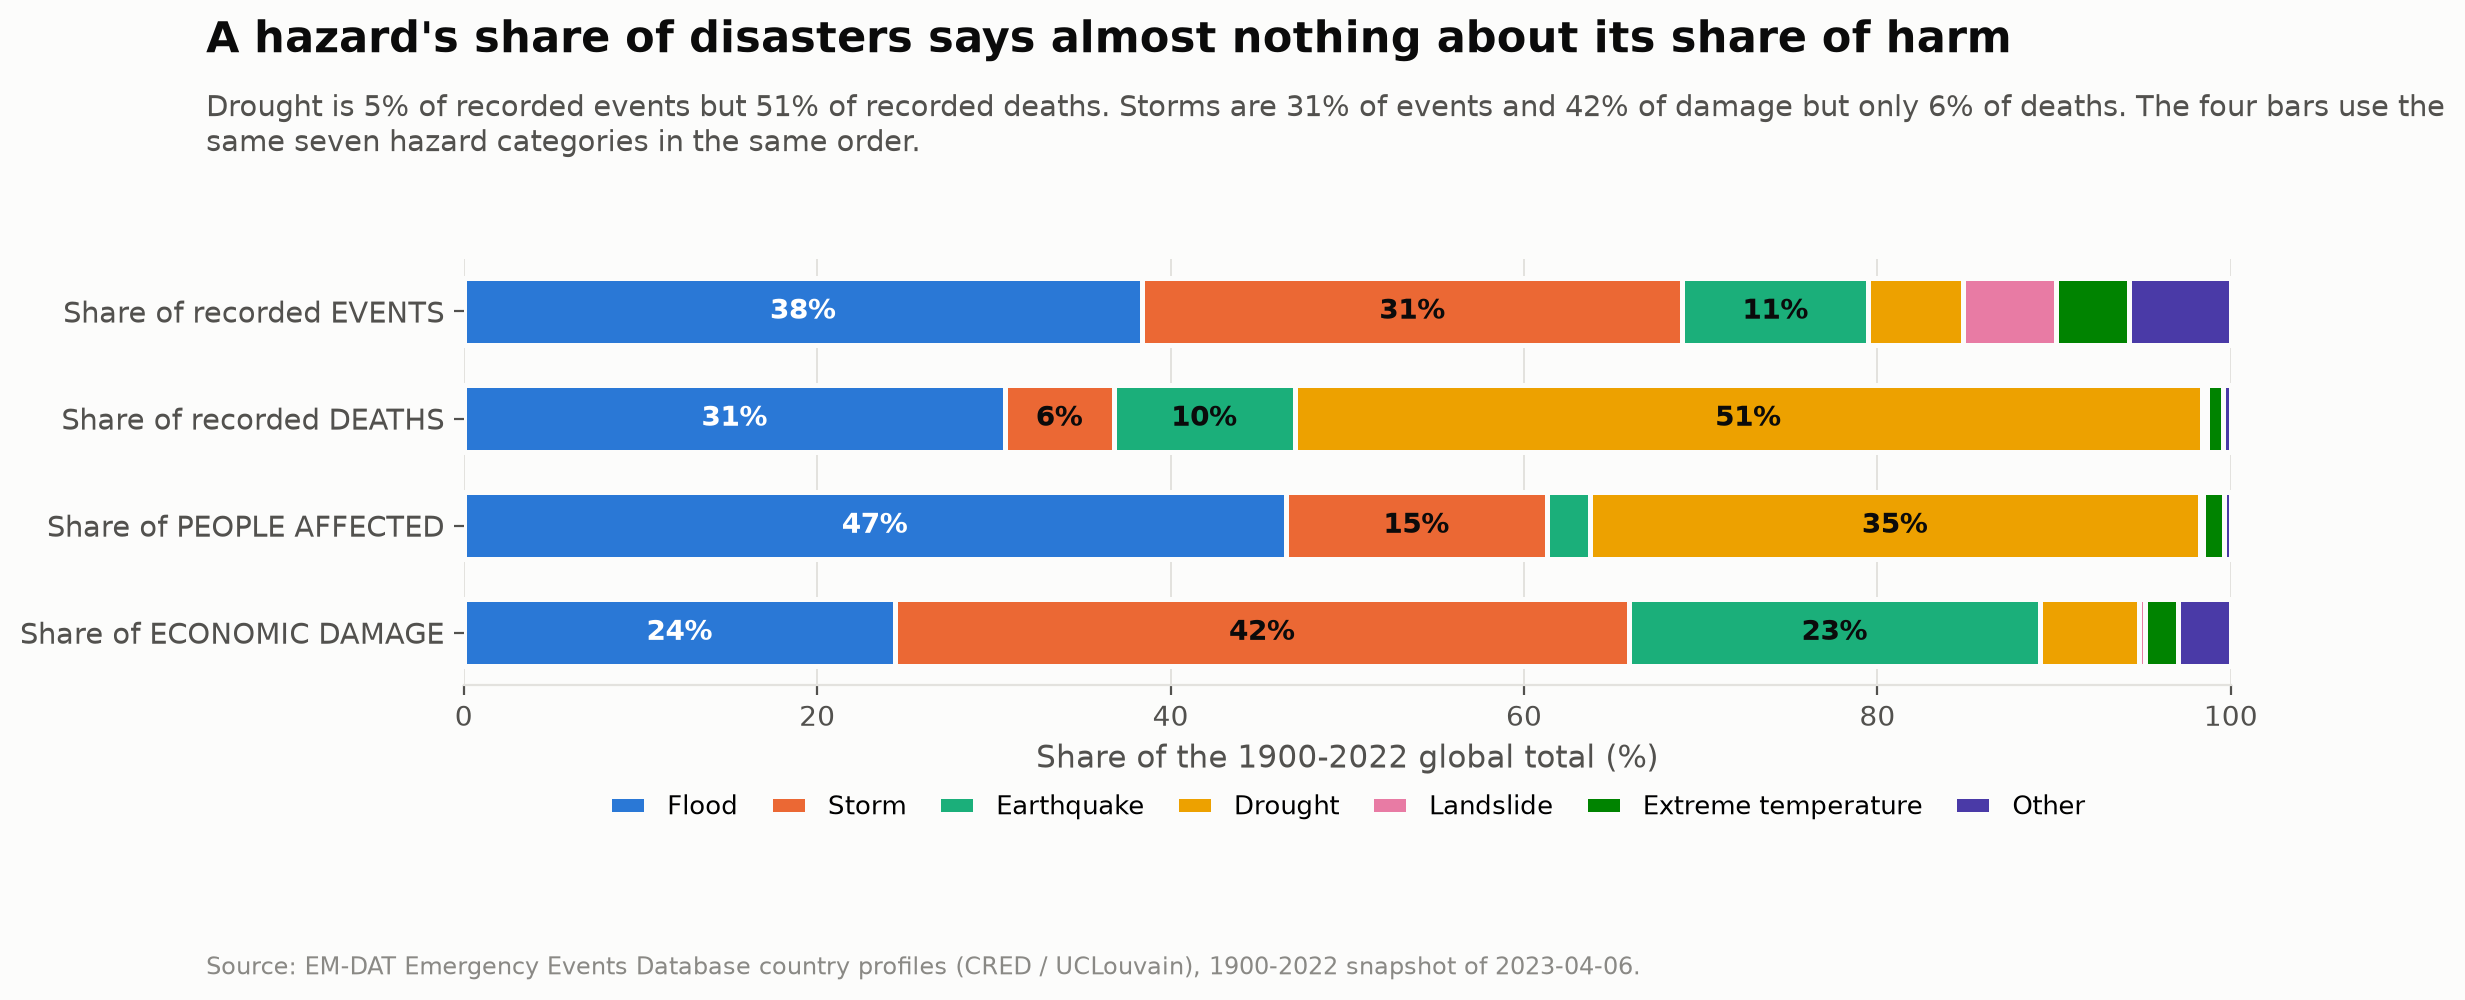
\includegraphics[width=\figw]{Fig13}
\caption[Each hazard's share of four burdens]{\textbf{Share of the global total
held by each hazard type, for four different burdens.} 100\%-stacked bars are
used because the question is composition, and the four bars use the same seven
categories in the same colour order so the eye can track a single hazard down the
chart.}
\label{fig:signature}
\end{figure}

\howto Four bars, one per burden, each stretched to the full width so that
each represents 100\% of that burden. The width of a coloured segment is the
share of that burden attributable to one hazard, and segments of 6\% or more
carry their percentage. The crucial detail is that all four bars use the same
seven hazards in the same left-to-right colour order --- so a single hazard can
be tracked straight down the chart, and a hazard whose segment changes width
between bars is one whose share of events differs from its share of harm.
Table~\ref{tab:shares} gives the exact numbers.

\inference This is the key chart of Task Set C, and it shows that a hazard's
share of \emph{events} predicts almost nothing about its share of \emph{harm}
(Table~\ref{tab:shares}). \textbf{Drought is 5\% of events and 51\% of deaths.}
Storms are the mirror image: 31\% of events and 42\% of the money, but only 6\%
of the deaths. Earthquakes are the concentrated destroyer --- a tenth of events,
a quarter of the damage, but only 2.4\% of people affected, because they strike
hard over small areas. Floods are the great displacer: they affect the most
people (46.5\%) while being neither the deadliest nor the costliest per event.

\begin{table}[H]
\centering
\caption{Each hazard's share of four different global burdens, 1900--2022. The
four columns are the four bars of Figure~\ref{fig:signature}.}
\label{tab:shares}
\small
\begin{tabular}{@{}l r r r r@{}}
\toprule
\textbf{Hazard} & \textbf{Share of} & \textbf{Share of} & \textbf{Share of} & \textbf{Share of}\\
                & \textbf{events}   & \textbf{deaths}   & \textbf{affected} & \textbf{damage}\\
\midrule
Flood       & 38.4\% & 30.6\%          & \textbf{46.5\%} & 24.4\%\\
Storm       & 30.6\% & \textbf{6.1\%}  & 14.8\%          & \textbf{41.5\%}\\
Earthquake  & 10.5\% & 10.3\%          & 2.4\%           & 23.3\%\\
Drought     & \textbf{5.3\%} & \textbf{51.3\%} & 34.5\%  & 5.6\%\\
\bottomrule
\end{tabular}
\end{table}

\taskhead{C1.2}{Relate: deadly versus costly}

\begin{figure}[H]
\centering
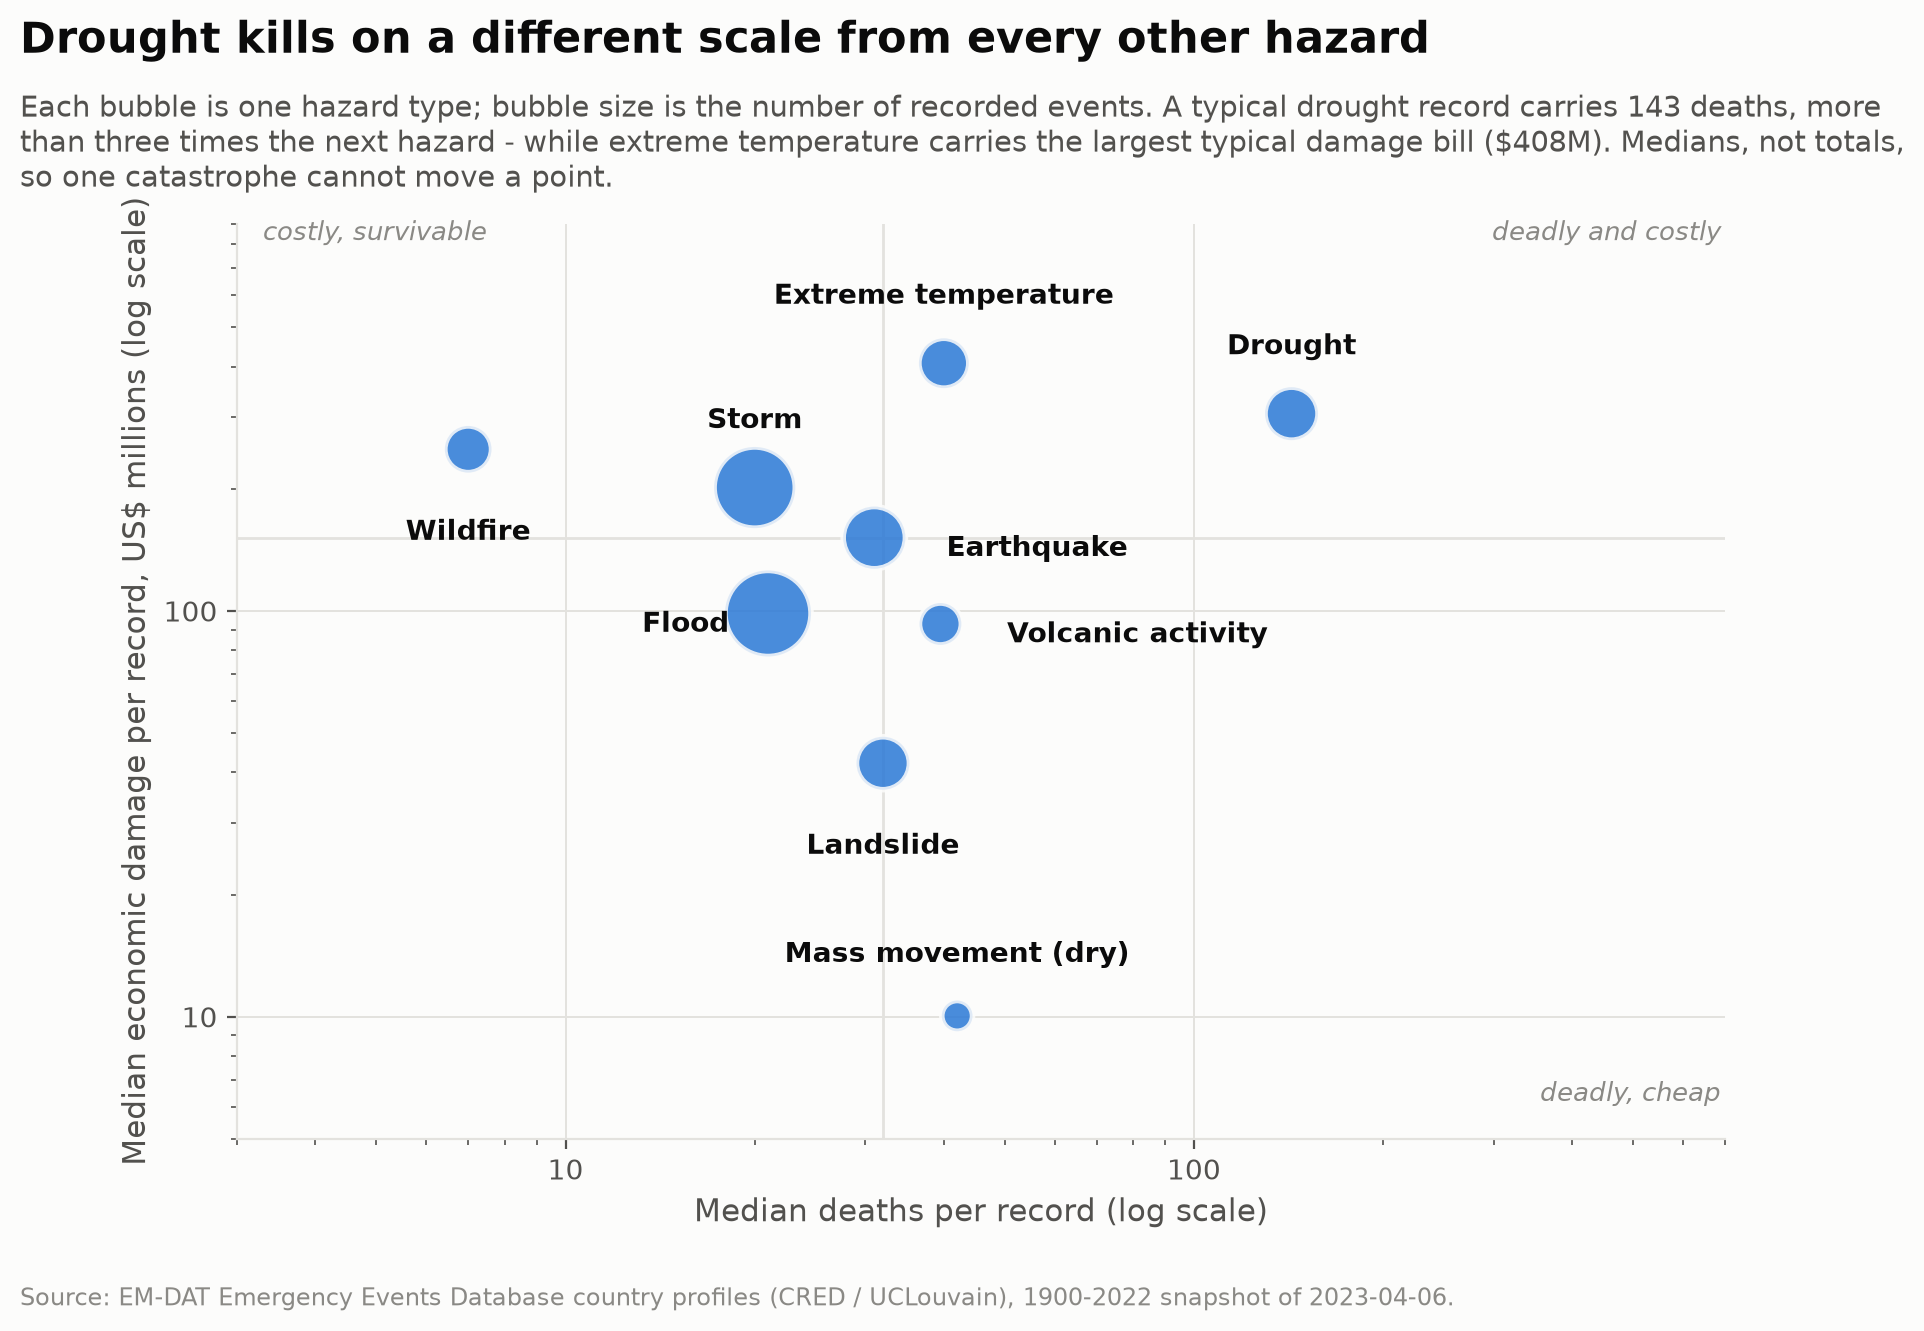
\includegraphics[width=\figw]{Fig14}
\caption[Deadliness against cost per hazard]{\textbf{Median deaths against median
damage per record}, one bubble per hazard type, bubble area proportional to the
number of events, both axes logarithmic. Medians rather than totals, so that a
single catastrophe cannot move a hazard's position. A single hue is used because
bubble identity is carried by direct labels, not by colour.}
\label{fig:scatter}
\end{figure}

\howto Each bubble is one hazard type, positioned by two medians: how deadly
a typical record of that hazard is (horizontal) and how expensive a typical
record is (vertical). Both axes are logarithmic, so a bubble twice as far right
is far more than twice as deadly. Bubble area is proportional to how many events
of that hazard were recorded, so a large bubble is a common hazard. The faint
grey crosshair sits at the median of each axis and divides the plane into the
four labelled quadrants. Medians rather than totals are used so that one
catastrophe cannot drag a hazard across the plot.

\inference Drought sits alone on the right: a typical drought record carries
\textbf{143 deaths}, more than three times the next hazard. The costliest
\emph{typical} hazard is a different one --- extreme temperature, at a median
\textbf{\$408 million} per record --- and wildfire sits in the opposite corner
from drought, expensive (a median \$250 million) but almost harmless to life (a
median of 7 deaths). Hazards do not lie on a single ``severity'' axis; they
occupy distinct positions in a deadliness--cost plane.

\taskhead{C1.3}{Trend: the real cost through time}

\begin{figure}[H]
\centering
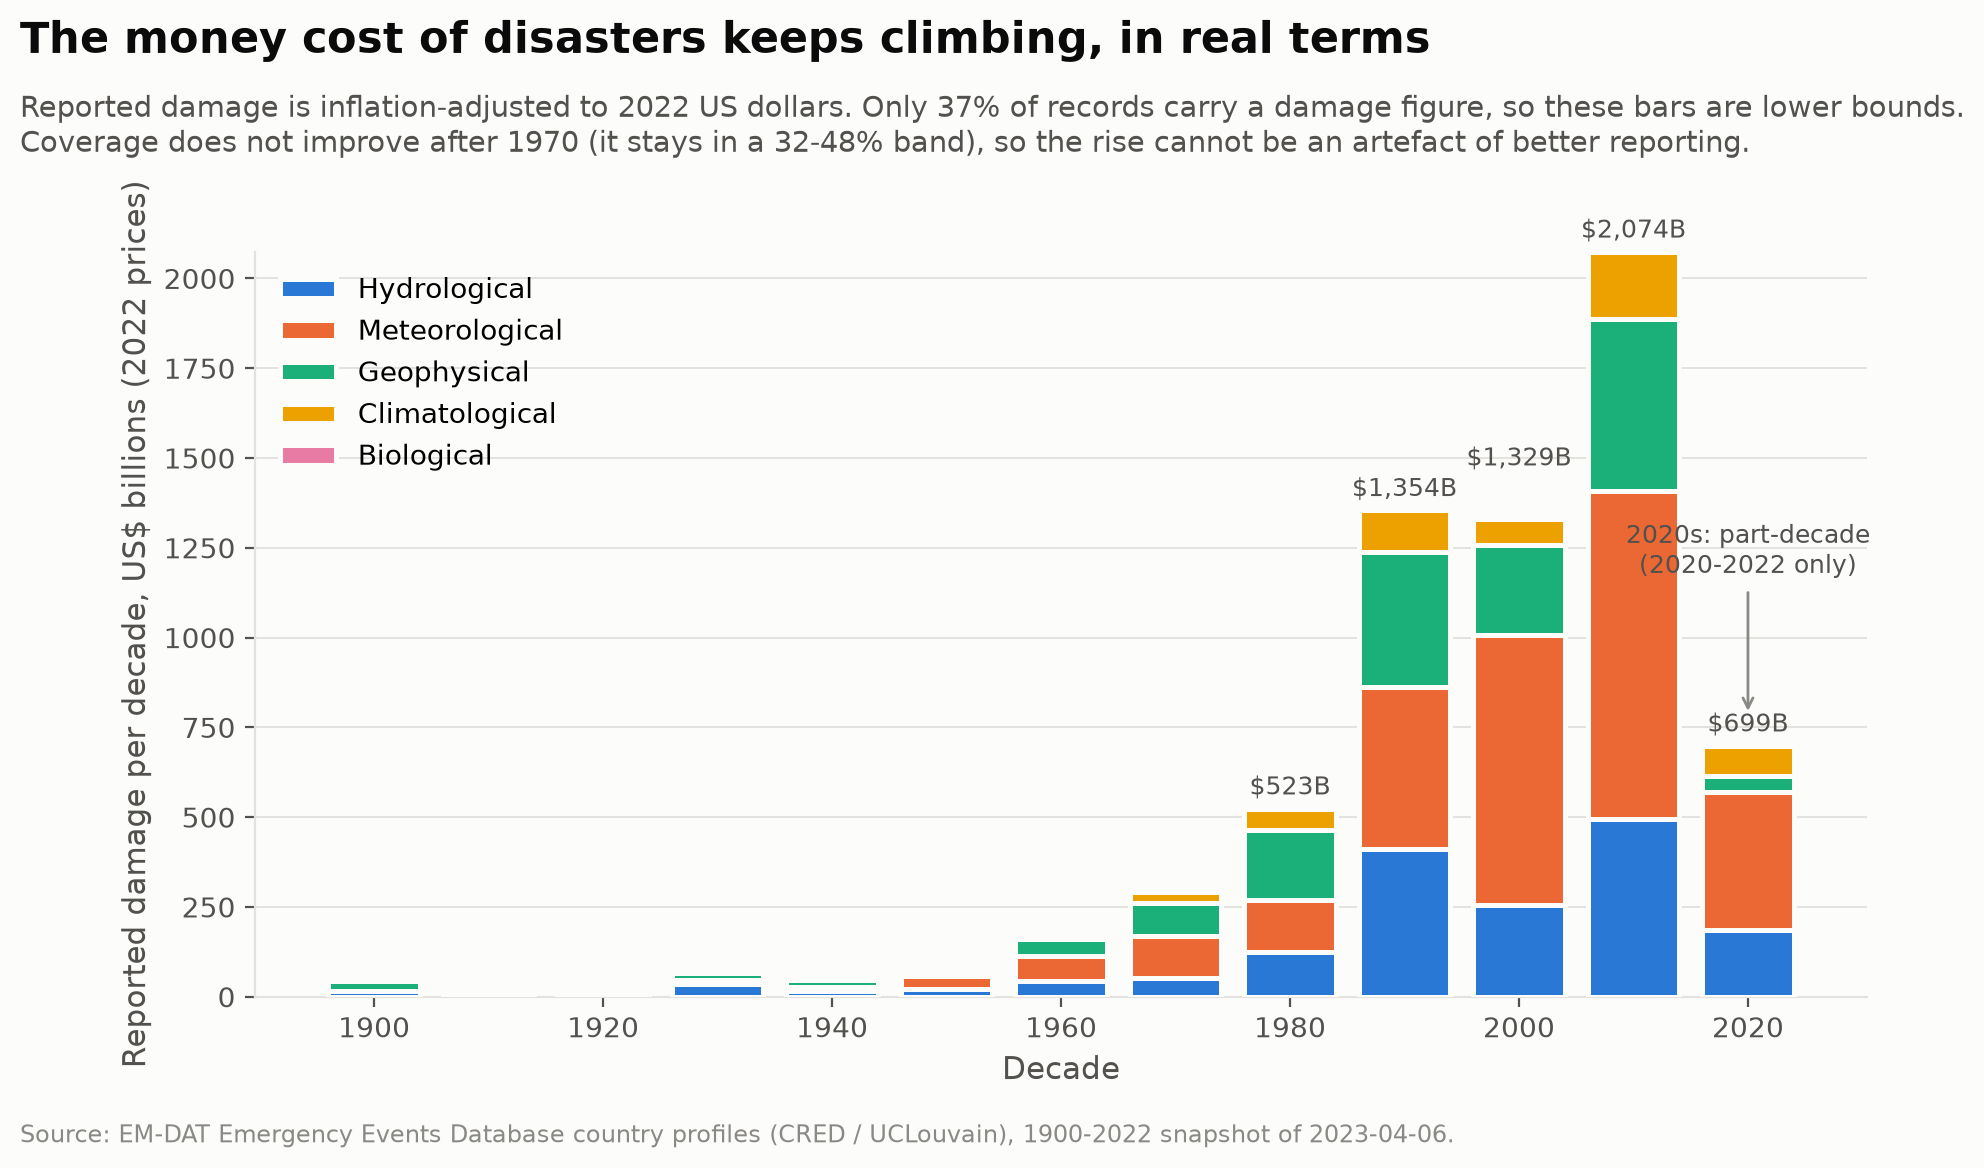
\includegraphics[width=\figw]{Fig15}
\caption[Real economic damage by decade]{\textbf{Reported economic damage per
decade in constant 2022 US dollars}, stacked by sub-group. Inflation adjustment
is essential over a 123-year window; the sub-group breakdown shows which hazards
drive the growth.}
\label{fig:damage}
\end{figure}

\howto The horizontal axis is the decade and the vertical axis is reported
economic damage in billions of US dollars, all converted to constant 2022 prices
so that decades are comparable. Segments are stacked by sub-group, so the height
of a segment is that sub-group's damage and the height of the whole bar is the
decade total, labelled above the taller bars. Note that the 2020s bar covers only
three years and is annotated as such.

\inference Real damage rises relentlessly: \textbf{\$1{,}354 billion in the
1990s, \$1{,}329 billion in the 2000s, and \$2{,}074 billion in the 2010s} ---
the costliest decade on record --- and the 2020s are already at \$699 billion
with only three years counted. Meteorological damage (storms) is the largest and
fastest-growing component. Because the share of records carrying a damage figure
does \textbf{not} improve after 1970, this rise cannot be dismissed as better
reporting; if anything, flat-to-declining coverage means the true rise is
steeper.

\taskhead{C1.4}{Compare: which hazards became survivable?}

\begin{figure}[H]
\centering
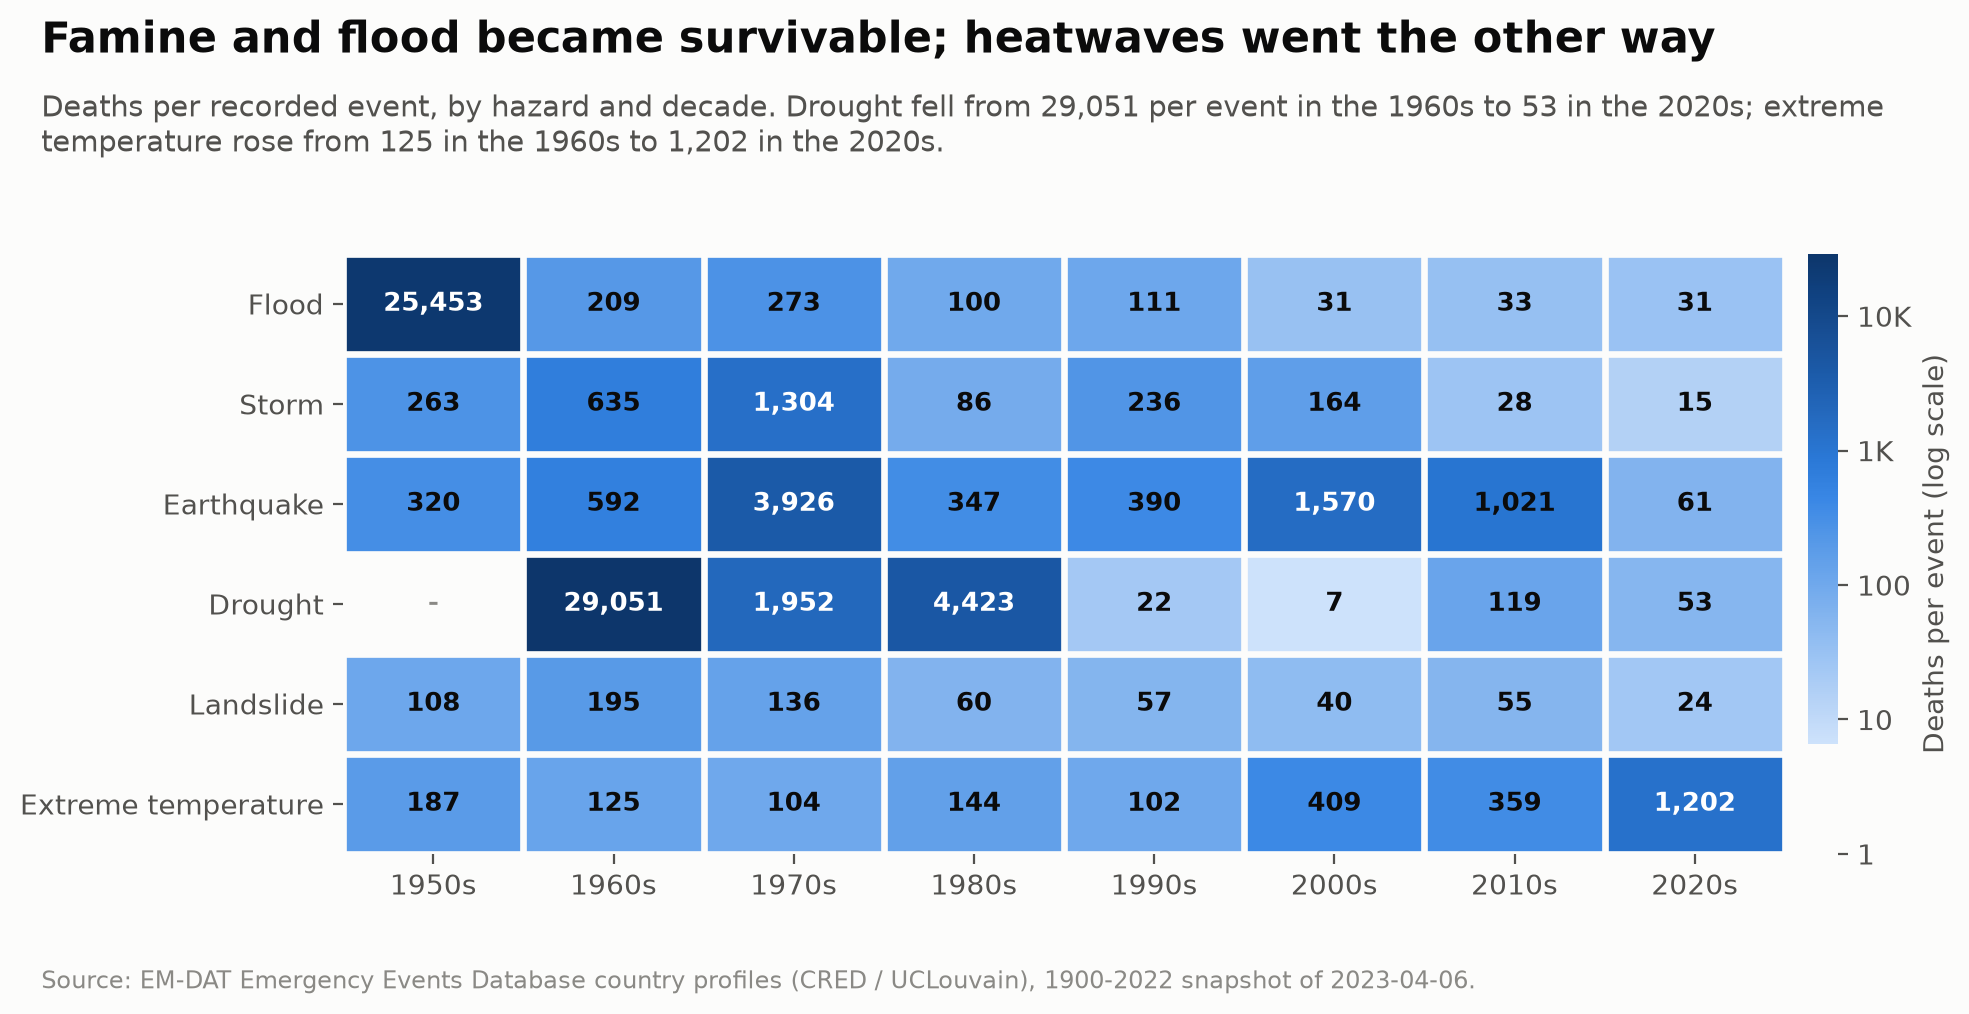
\includegraphics[width=\figw]{Fig16}
\caption[Lethality by hazard and decade]{\textbf{Deaths per recorded event, by
hazard and decade, 1950s--2020s.} A heatmap is the right form for a categorical
$\times$ ordinal grid of a single measure; values are printed in every cell so
the reader never has to estimate a number from colour, and the sequential blue
ramp is logarithmic. The 2020s column covers 2020--2022 only.}
\label{fig:heatmap}
\end{figure}

\howto A grid, not a chart with axes: each row is a hazard, each column a
decade, and each cell holds one number --- deaths per recorded event for that
hazard in that decade. The number is printed in every cell, so colour is a
reading aid rather than the data itself; the blue ramp runs pale for low to dark
for high on a logarithmic scale. A dash means that hazard has no recorded events
in that decade. Read \emph{along a row} to see whether a hazard became more or
less survivable over time, and \emph{down a column} to compare hazards within one
decade.

\inference The improvement is real but uneven, and one hazard moves the wrong
way:

\begin{itemize}
\item \textbf{Drought collapsed}: 29{,}051 deaths per event in the 1960s
  $\rightarrow$ 119 in the 2010s $\rightarrow$ 53 in the 2020s. Famine
  early-warning systems and food logistics are the plausible explanation.
\item \textbf{Flood collapsed}: 25{,}453 in the 1950s $\rightarrow$ 33 in the 2010s.
\item \textbf{Storm collapsed}: 1{,}304 in the 1970s $\rightarrow$ 28 in the
  2010s $\rightarrow$ 15 in the 2020s. Cyclone forecasting and evacuation.
\item \textbf{Earthquake did not improve}: 320 in the 1950s, 1{,}570 in the
  2000s, 1{,}021 in the 2010s. Earthquakes give no warning, so the interventions
  that tamed floods and droughts do not apply.
\item \textbf{Extreme temperature got worse}: 125 in the 1960s $\rightarrow$ 409
  in the 2000s $\rightarrow$ \textbf{1{,}202 in the 2020s}. Heatwaves are the one
  hazard in this dataset becoming \emph{more} lethal per event.
\end{itemize}

\taskhead{C1.5}{Correlate: the decoupling}

\begin{figure}[H]
\centering
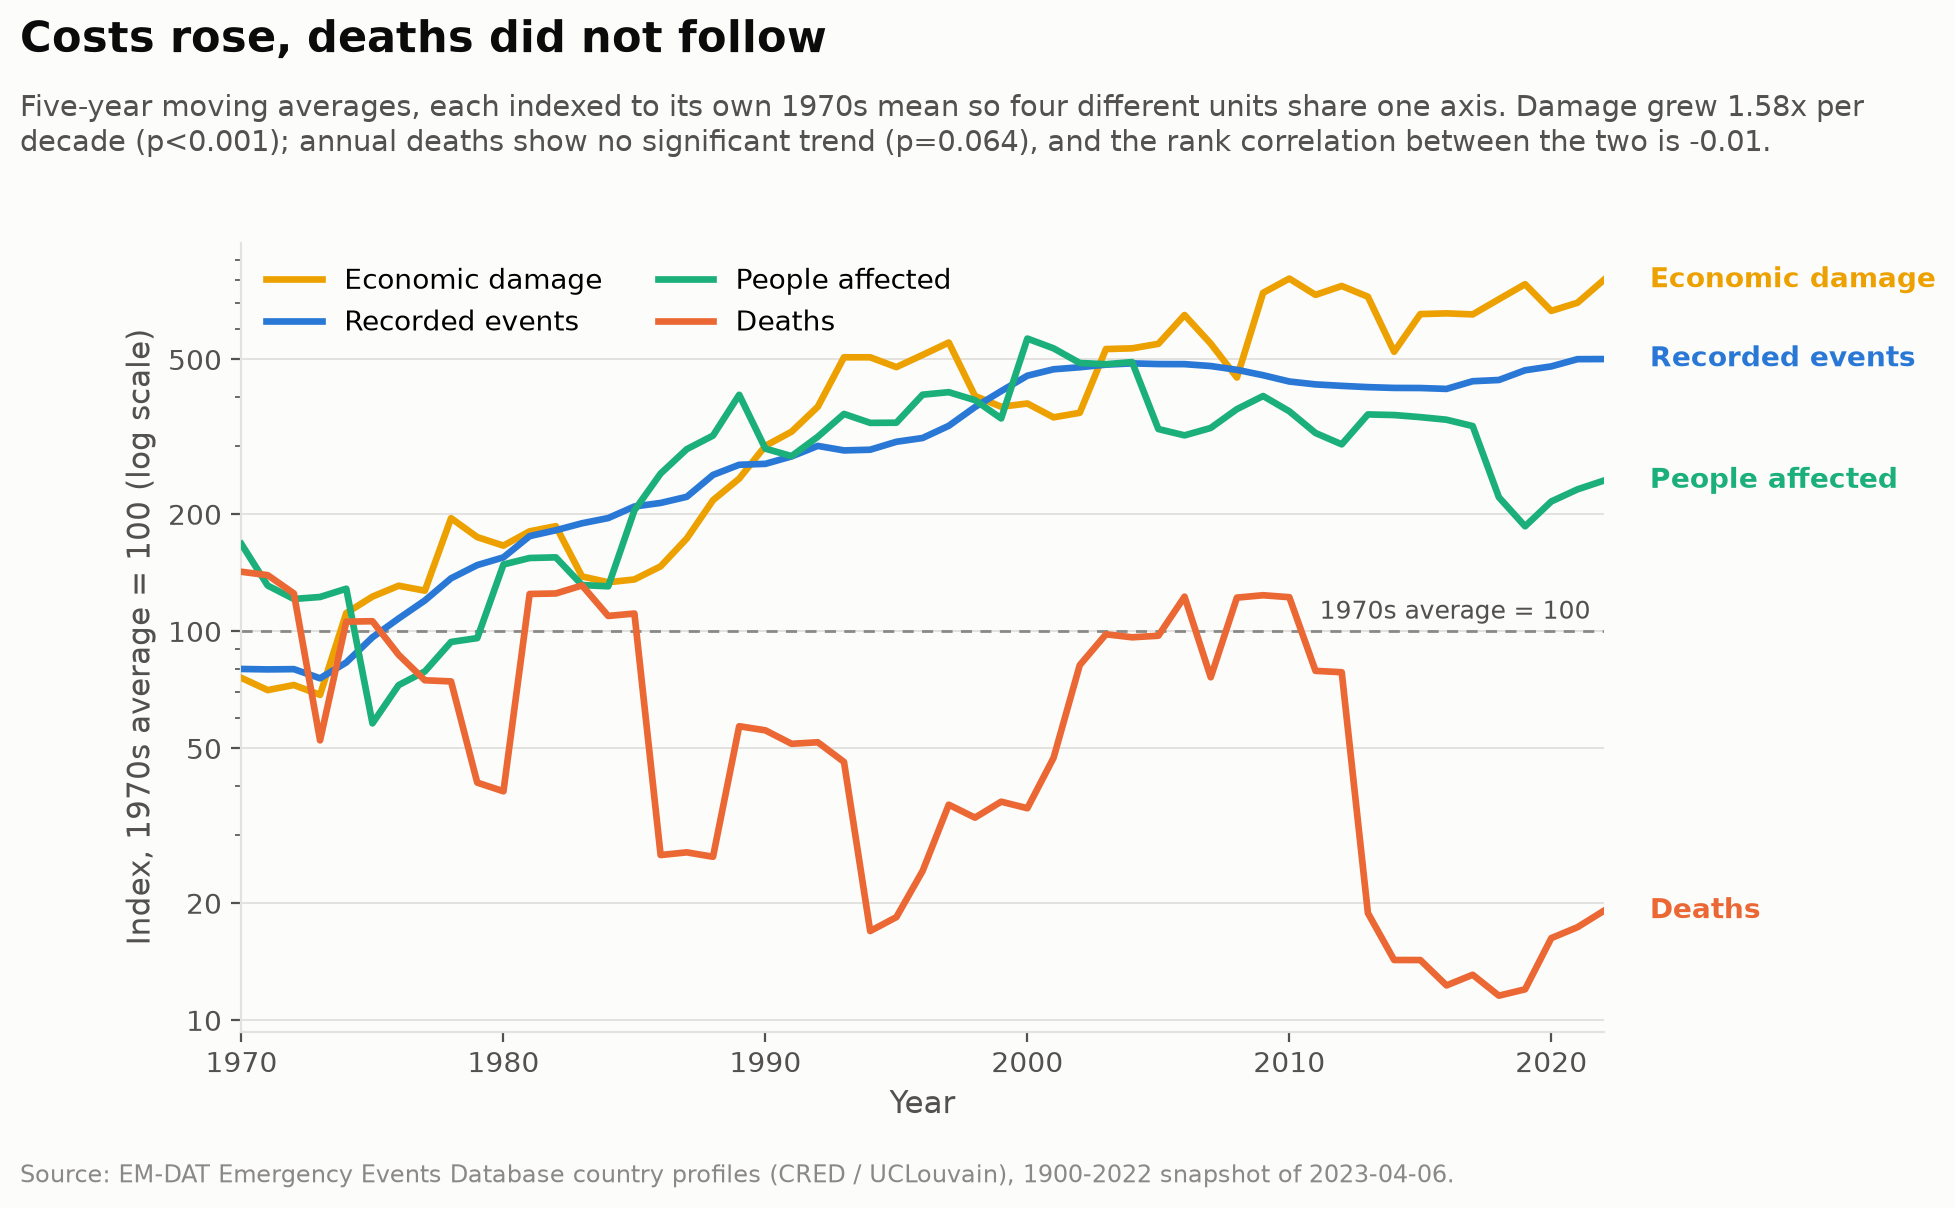
\includegraphics[width=\figw]{Fig17}
\caption[Indexed events, affected, deaths and damage]{\textbf{Recorded events,
people affected, deaths and economic damage, 1970--2022}, each as a five-year
moving average indexed to its own 1970s mean. Indexing to a common base of 100 is
what allows four different units to share a single axis honestly, instead of
resorting to a dual axis.}
\label{fig:decoupling}
\end{figure}

\howto The four measures have four different units, so none is plotted
directly. Instead each series is divided by its own 1970s average and multiplied
by 100 --- so every line starts near 100, and a value of 200 means ``twice the
1970s level \emph{for that measure}''. This is what lets four incompatible units
share one honest axis instead of a dual axis. The vertical axis is logarithmic so
proportional changes are comparable, each line is a five-year moving average to
suppress single-year spikes, and the dashed line marks the 1970s baseline of 100.
Lines that rise together have moved together; lines that separate have decoupled.

\inference Over 1970--2022 the four measures separate cleanly. Fitting a
log-linear trend to each annual series gives Table~\ref{tab:trends}. Events,
damage and people affected all rise significantly. \textbf{Annual deaths show no
statistically significant trend at all} ($p = 0.064$), and the Spearman rank
correlation between annual deaths and annual damage is $\mathbf{-0.01}$ ---
effectively zero. Median annual damage rose from \$36 billion (1970--89) to
\$179 billion (2003--22), a five-fold increase, while median annual deaths went
from 25{,}586 to 19{,}265. What \emph{is} significant is deaths \textbf{per
event}, falling by a factor of 0.58 each decade. The world is not suffering fewer
disasters or cheaper ones; it is surviving each one far better.

\begin{table}[H]
\centering
\caption{Log-linear trend fits to the annual series, 1970--2022. Exact
$p$-values are reproduced in \texttt{code/facts\_output.txt}.}
\label{tab:trends}
\small
\begin{tabular}{@{}l r r r@{}}
\toprule
\textbf{Measure} & \textbf{Change per decade} & \textbf{$p$} & \textbf{$R^2$}\\
\midrule
Recorded events        & $\times 1.43$ & $< 0.001$ & 0.82\\
Economic damage (real) & $\times 1.58$ & $< 0.001$ & 0.63\\
People affected        & $\times 1.36$ & $< 0.001$ & 0.29\\
\textbf{Deaths}        & $\mathbf{\times 0.83}$ \textbf{--- not significant} & \textbf{0.064} & \textbf{0.07}\\
Deaths \emph{per event}& $\times 0.58$ & $< 0.001$ & 0.38\\
\bottomrule
\end{tabular}
\end{table}

%=======================================================================
\section{The Data Story}
\label{sec:story}
%=======================================================================

Read in sequence, the fifteen charts tell one story in four movements.

\textbf{1. The record grows --- but so does the recording.}
Figures~\ref{fig:types}--\ref{fig:reporting} establish what the dataset contains
and immediately undercut the naive reading of it. Recorded events grew 52-fold
from the 1900s to the 2000s, but 91\% of the record falls in 43\% of the years,
and damage reporting covers at most half the records. Counts are unreliable;
rates are not.

\textbf{2. Yet the world got dramatically better at surviving.}
Figure~\ref{fig:deaths} shows deaths per recorded event falling 99.4\% across the
century, and Figure~\ref{fig:decoupling} confirms it is the only mortality trend
in the modern era that is statistically significant. Figure~\ref{fig:heatmap}
localises the improvement: droughts, floods and storms --- the hazards that give
warning --- became survivable, while earthquakes, which do not, did not improve
at all.

\textbf{3. But ``the world'' is the wrong unit.}
Figures~\ref{fig:mapevents}--\ref{fig:lethality} show the improvement is not
evenly distributed. Occurrence is global; death is not. Two countries carry half
of all recorded deaths, and among the twenty most disaster-exposed countries
lethality spans three orders of magnitude. The United States leads the world in
recorded disasters and in dollar losses while ranking 23rd in deaths --- wealth
converts disaster exposure into property damage instead of mortality.

\textbf{4. And the bill keeps growing.}
Figures~\ref{fig:signature}--\ref{fig:damage} show that the hazards that kill
(drought) and the hazards that cost (storms, earthquakes) are largely different
hazards, and that real damage reached a record \$2.07 trillion in the 2010s.
Figure~\ref{fig:decoupling} closes the loop: costs and deaths have decoupled
almost perfectly (rank correlation $-0.01$).

\callout{\textbf{Answer to the guiding question.} The burden of natural disasters
has grown, but not in the way the headline suggests. \emph{Exposure} has risen
--- more assets, more people, and much better reporting. \emph{Vulnerability} has
fallen sharply, and that fall is the real achievement of the last century. And
the fall is unevenly shared, incomplete for hazards that give no warning, and
reversing outright for extreme heat.}

And one honest caveat on our own headline, from Figure~\ref{fig:trimmed}: most of
the century-scale fall in \emph{total} deaths is the disappearance of a handful
of mega-catastrophes rather than a broad decline in ordinary disaster deaths. The
per-event improvement is robust; the total-deaths improvement is more fragile
than it first appears.

%=======================================================================
\section{Consolidated Inferences}
%=======================================================================

\begin{enumerate}
\item Floods and storms are 69\% of all recorded events; drought is 5.3\% of
  events but 51.3\% of deaths.
\item Recorded events grew 52$\times$ from the 1900s to the 2000s, but 91\% of
  the record sits in 43\% of the years --- the count measures reporting as much
  as hazard.
\item Deaths per recorded event fell 99.4\%, from $\approx$19{,}900 (1900s) to
  $\approx$129 (2010s).
\item That fall is driven by the disappearance of mega-catastrophes; excluding
  each decade's three worst records, residual deaths show no downward trend
  (2000s: 390k $>$ 1900s: 117k).
\item All 225 countries appear in the record, but 2 countries hold half of all
  deaths and 5 countries hold 87.1\%.
\item The United States is 1st in events and damage but 23rd in deaths;
  Bangladesh is 3rd in deaths but 23rd in damage.
\item Among the 20 most disaster-exposed countries, deaths per event span a
  factor of $\approx$1{,}000 (China 11{,}139 $\rightarrow$ Australia 11).
\item A hazard's share of events does not predict its share of harm: storms are
  31\% of events but 6\% of deaths; drought is 5\% of events but 51\% of deaths.
\item Real economic damage reached a record \$2.07 trillion in the 2010s and is
  rising $\times 1.58$ per decade ($p < 0.001$).
\item Annual deaths show no significant trend since 1970 ($p = 0.064$); the rank
  correlation between annual deaths and annual damage is $-0.01$. Costs and
  mortality have decoupled.
\item Drought lethality fell from 29{,}051 to 53 deaths per event; earthquake
  lethality did not improve; \textbf{extreme-temperature lethality rose roughly
  ten-fold} (125 $\rightarrow$ 1{,}202).
\item Wealth appears to convert disaster exposure into property loss rather than
  death --- the clearest policy-relevant pattern in the dataset.
\end{enumerate}

%=======================================================================
\section{Limitations and Threats to Validity}
\label{sec:limits}
%=======================================================================

\begin{itemize}
\item \textbf{Reporting bias is not correctable.} We mitigate it by preferring
  rates to counts and by restricting statistical trend fits to 1970 onward, but
  pre-1970 counts remain unusable as a hazard measure.
\item \textbf{Damage is under-reported} (36.9\% coverage), so all damage totals
  are lower bounds. Coverage does not improve after 1970, so the upward trend is
  not a coverage artefact.
\item \textbf{No population denominator.} Deaths per event is a severity proxy,
  not a risk rate. China and India's dominance in Figure~\ref{fig:mapdeaths}
  partly reflects population, and this is stated wherever the figure is
  discussed.
\item \textbf{Rows are aggregates}, so per-event values are cell averages, not
  per-disaster values.
\item \textbf{Historical states} (Soviet Union, Yugoslavia, Czechoslovakia and
  four others) appear as countries and are flagged in the cleaned extract.
\item \textbf{The 2020s are a part-decade} (2020--2022) and are annotated as such
  in Figures~\ref{fig:reporting}, \ref{fig:deaths}, \ref{fig:damage} and
  \ref{fig:heatmap}.
\item \textbf{No epidemics.} COVID-19 and all disease events are absent from this
  file; nothing here speaks to biological disaster risk.
\item \textbf{Correlation is not causation.} Section~\ref{sec:story}'s
  attribution of falling lethality to warning systems and response capacity is an
  interpretation consistent with the pattern in Figure~\ref{fig:heatmap}, not
  something this dataset can establish on its own.
\end{itemize}

%=======================================================================
\section{Tools and Reproducibility}
\label{sec:repro}
%=======================================================================

Table~\ref{tab:tools} lists the tool used for each component of the submission.

\begin{table}[H]
\centering
\caption{Tools used for each component of the submission.}
\label{tab:tools}
\small
\begin{tabularx}{\linewidth}{@{}>{\raggedright\arraybackslash}p{6.2cm} X@{}}
\toprule
\textbf{Component} & \textbf{Tool}\\
\midrule
Data cleaning and analysis & Python 3.12, pandas 3.0, NumPy, SciPy\\
Statistical charts (Figures \ref{fig:types}--\ref{fig:trimmed},
  \ref{fig:leaderboards}--\ref{fig:decoupling}) & Matplotlib 3.11\\
Method diagrams (Figures \ref{fig:taskmap}, \ref{fig:pipeline}) & Matplotlib 3.11\\
Choropleth maps (Figures \ref{fig:mapevents}, \ref{fig:mapdeaths}) & Plotly 6.9 with Kaleido static export\\
Interactive dashboards and video demo & Tableau Public, reading \texttt{data/emdat\_clean\_tableau.csv}\\
This report & \LaTeX{} (\texttt{pdflatex}), source \texttt{report/DAS732\_A1\_Report.tex}\\
\bottomrule
\end{tabularx}
\end{table}

To regenerate every figure and rebuild this PDF from the raw CSV:

\begin{quote}\ttfamily
cd code\\
python run\_all.py
\end{quote}

\texttt{code/facts.py} and \texttt{code/facts2.py} re-derive \textbf{every
quantitative claim} made in this report; their output is saved as
\texttt{code/facts\_output.txt} and \texttt{code/facts2\_output.txt} so that any
number here can be traced to the line that produced it.
\texttt{code/check\_report.py} then re-reads this \LaTeX{} source and asserts
every figure quoted in it against the data, so a stale number cannot survive a
rebuild. \texttt{Tableau\_Guide.md} gives step-by-step instructions for
rebuilding six demonstrable views in Tableau from the cleaned extract, for the
video demo.


%=======================================================================
\section{Supplementary Figures}
\label{sec:supp}
%=======================================================================

The fifteen figures of Sections~\ref{sec:taskA}--\ref{sec:taskC} answer the
guiding question on their own. The five below were produced afterwards to
pressure-test three specific claims that the main sequence asserts but does not
fully establish, and are reported here rather than in the main sequence so that
the data story stays the length the brief asks for. Each remains owned by the
member who owns the task set it extends.

\subsection*{Extending Task Set A --- separating hazard from record-keeping}
\addcontentsline{toc}{subsection}{Extending Task Set A}

Figure~\ref{fig:reporting} concluded that the event count is ``a joint
measurement of hazard and of reporting effort, and cannot be separated into the
two''. Figures~\ref{fig:typedecade} and \ref{fig:control} go further and
partially separate them.

\begin{figure}[H]
\centering
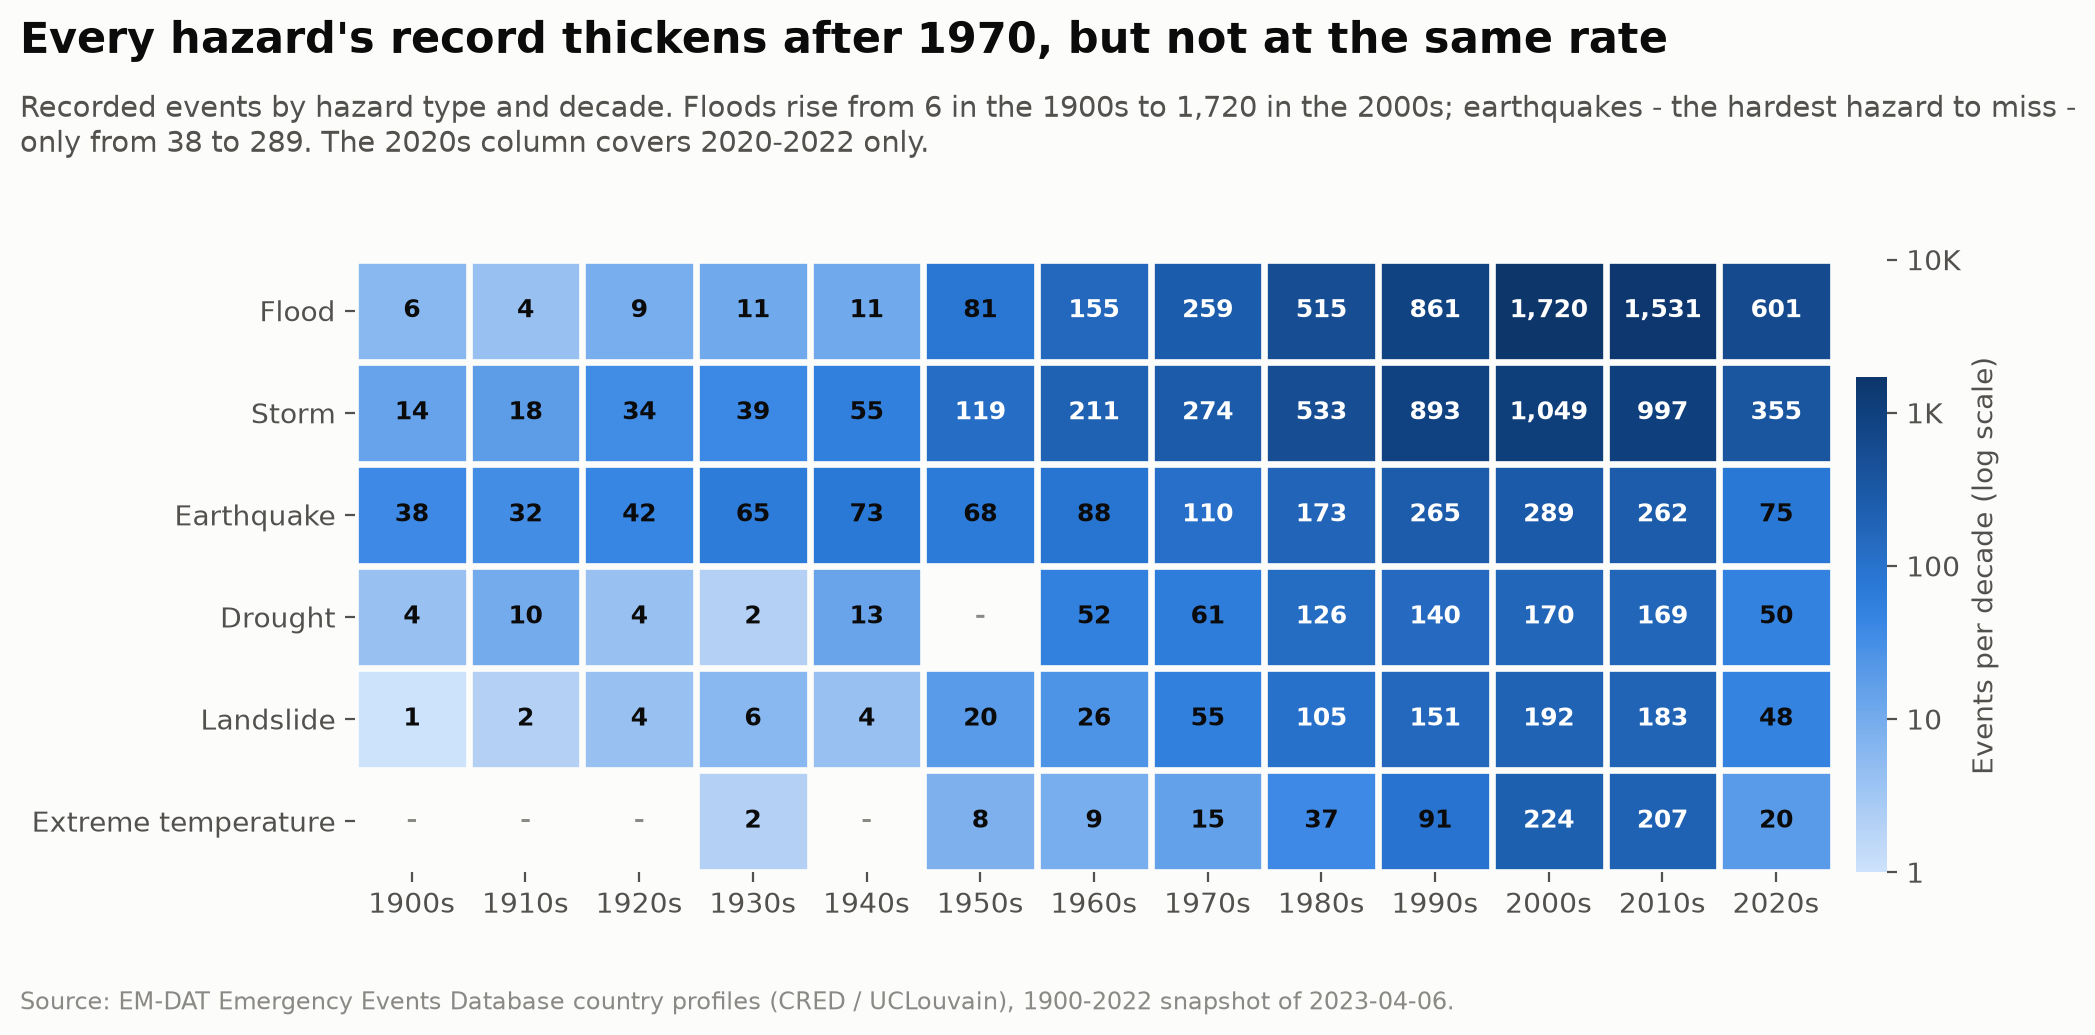
\includegraphics[width=\figw]{Fig18}
\caption[Recorded events by hazard and decade]{\textbf{Recorded events by hazard
type and decade.} The counts underlying the rates in
Figure~\ref{fig:control}; a heatmap is used so that thirteen decades and six
hazards fit in one view without thirteen separate bars per hazard.}
\label{fig:typedecade}
\end{figure}

\howto Each row is a hazard, each column a decade, and each cell is the number
of events recorded for that pair. The number is printed in every cell, so the
blue ramp (logarithmic, pale to dark) only ranks them at a glance. Read along a
row to see when that hazard's record thickened.

\inference Every hazard's record grows after 1970, but not by the same factor.
Floods rise from 6 events in the 1900s to 1,720 in the 2000s. Earthquakes ---
the hazard hardest to overlook --- rise only from 38 to 289. That difference is
the opening the next figure exploits.

\begin{figure}[H]
\centering
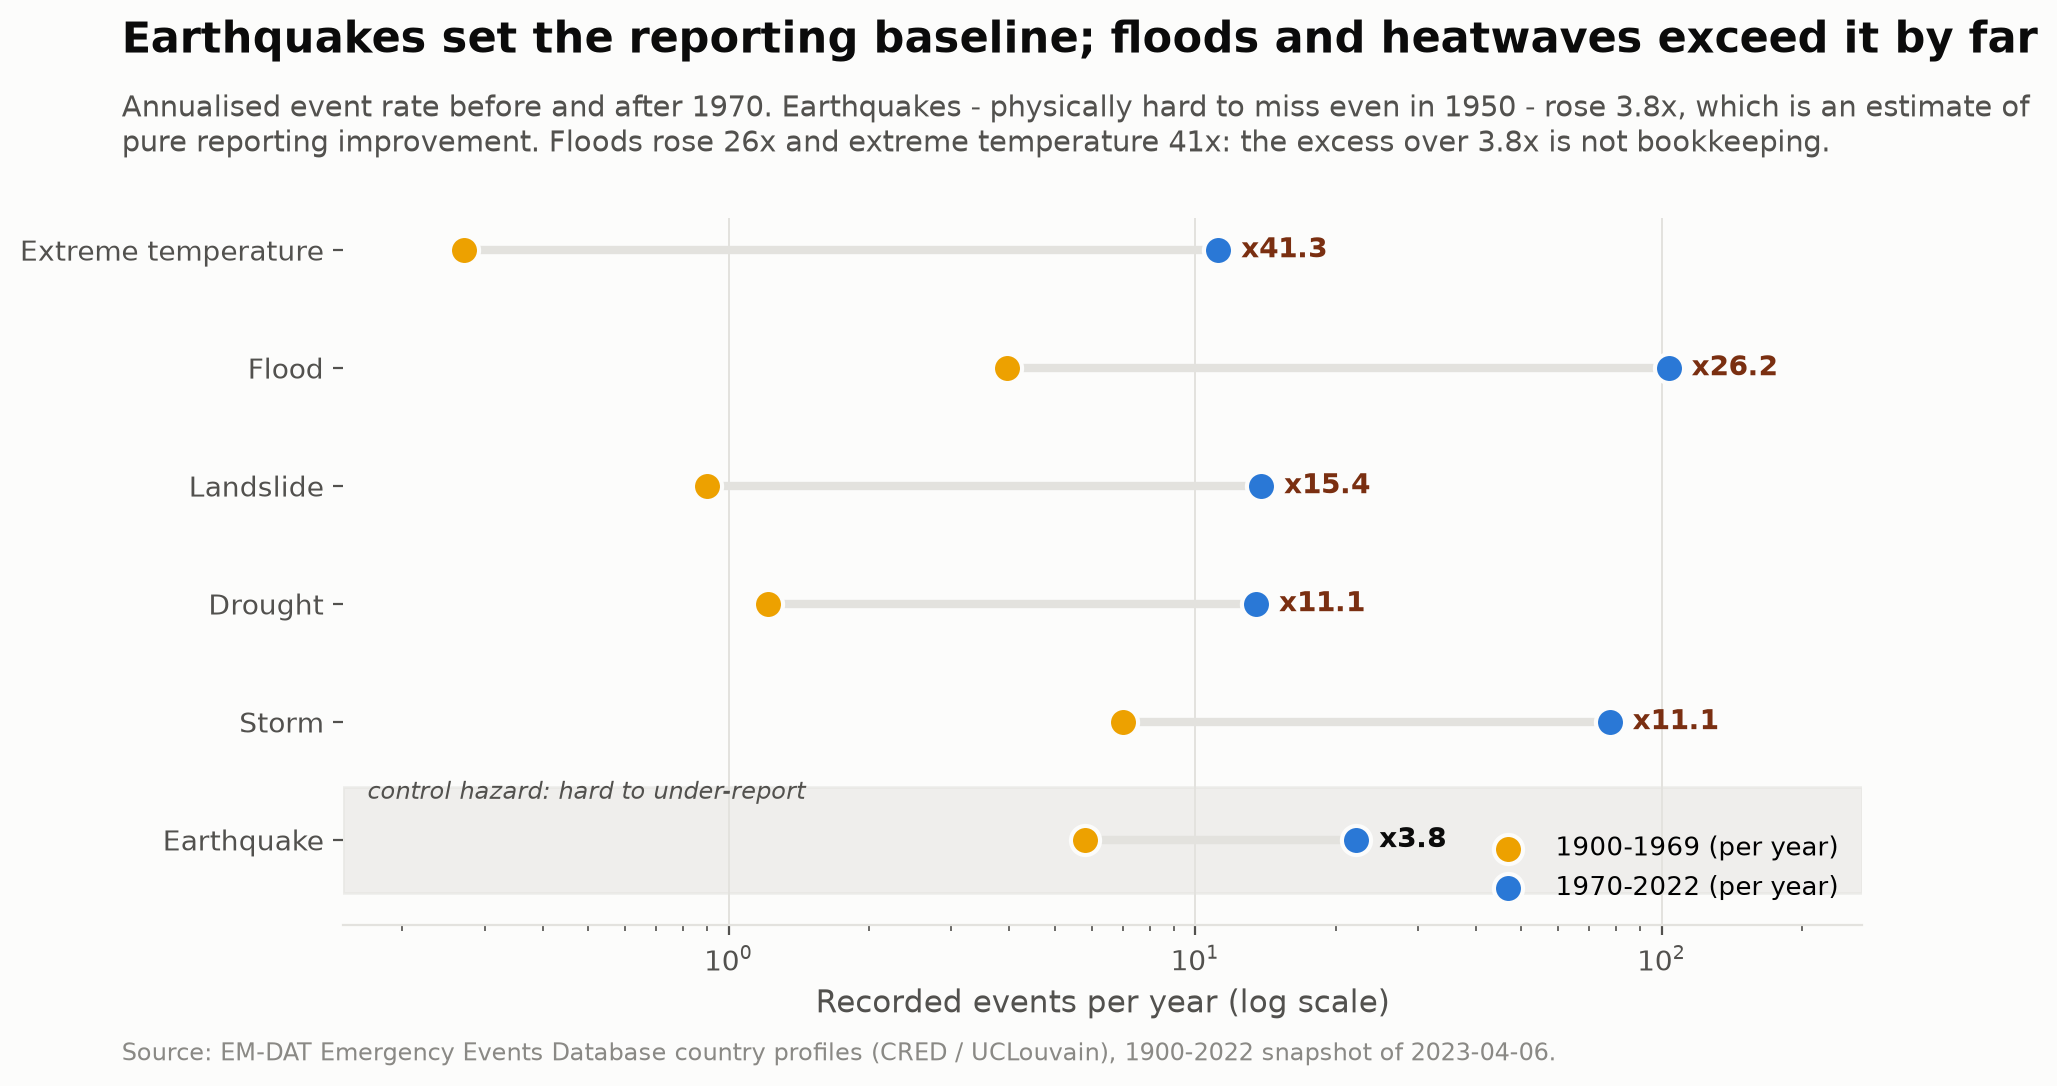
\includegraphics[width=\figw]{Fig19}
\caption[Pre- and post-1970 event rate with an earthquake control]{\textbf{Annualised
event rate before and after 1970, with earthquakes as a control hazard.} A
paired dot plot on a log axis: position encodes the rate, and the connector
length is the change. Earthquakes are used as a natural control because a
destructive earthquake is physically hard to miss even with 1950s
record-keeping, so its growth approximates \emph{pure} reporting improvement.}
\label{fig:control}
\end{figure}

\howto Two dots per hazard: the gold dot is the average number of events
recorded per year in 1900--1969, the blue dot the same for 1970--2022. Rates are
used rather than totals because the two eras are 70 and 53 years long. The
multiplier at the right of each row is blue-over-gold. The shaded row is the
control.

\inference Earthquakes rose $\times$3.8. If that is what better record-keeping
alone buys, then the excess above it is not bookkeeping: floods rose
$\times$26.2, extreme temperature $\times$41.3, landslides $\times$15.4, storms
and droughts $\times$11.1. This does not make the raw counts trustworthy in
absolute terms --- the control is an approximation, and earthquakes may
themselves be under-recorded early --- but it does show the post-1970 rise is
\emph{not} wholly an artefact, which Figure~\ref{fig:reporting} alone could not
establish.

\subsection*{Extending Task Set B --- testing the wealth reading directly}
\addcontentsline{toc}{subsection}{Extending Task Set B}

\begin{figure}[H]
\centering
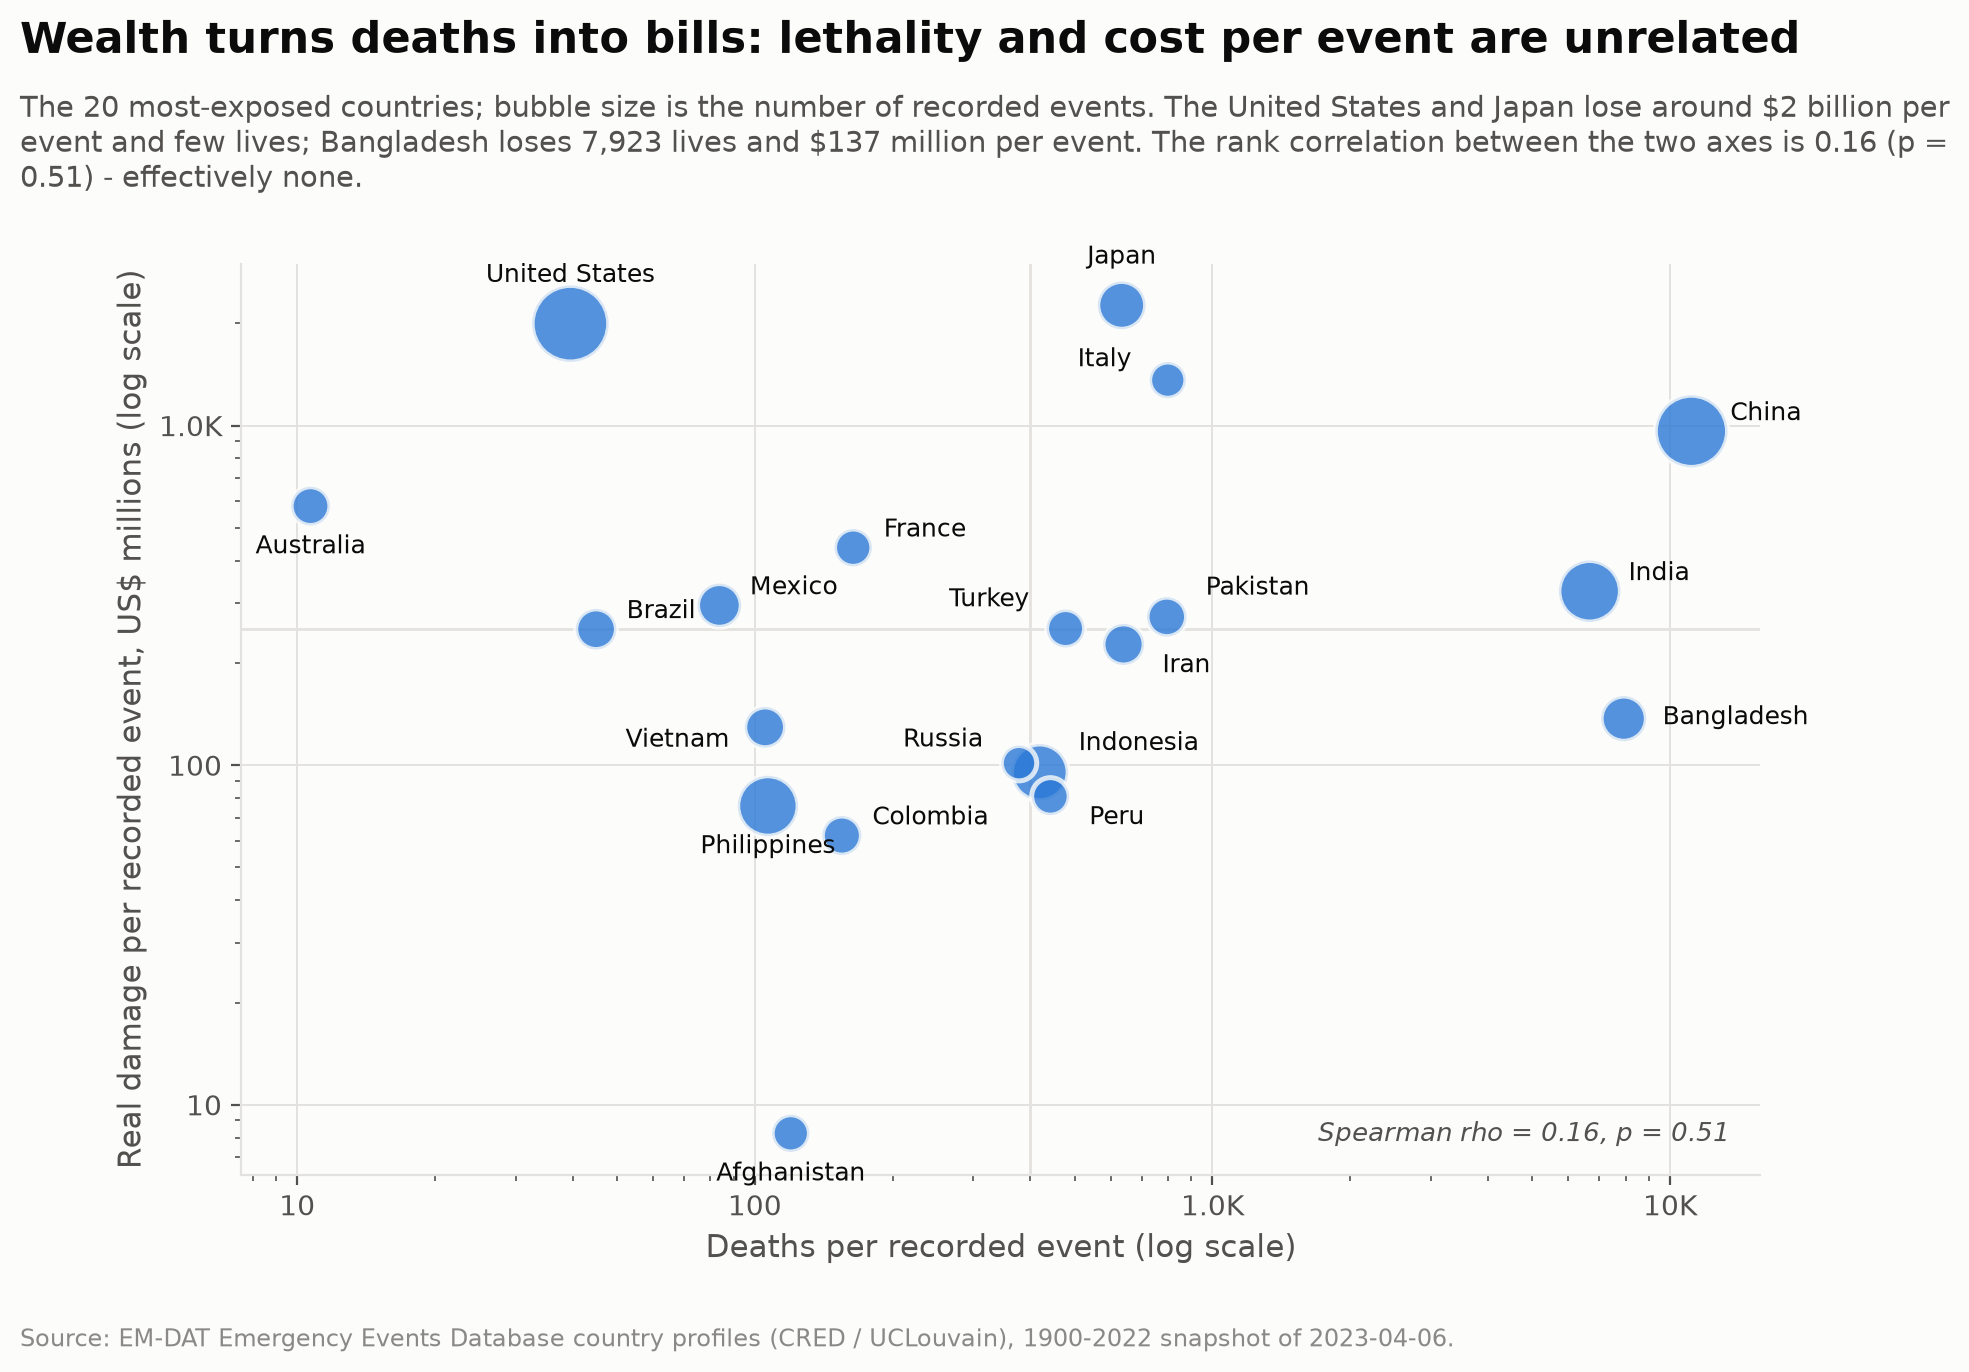
\includegraphics[width=\figw]{Fig20}
\caption[Country lethality against cost per event]{\textbf{Deaths per event
against damage per event, for the 20 most-exposed countries.} The same country
set as Figure~\ref{fig:lethality}, with the money axis added. Both axes are
logarithmic and bubble area is the number of recorded events.}
\label{fig:lethvscost}
\end{figure}

\howto Horizontal position is how many people a typical disaster kills in that
country; vertical position is what a typical disaster costs there. A country in
the lower right suffers deadly, cheap disasters; upper left, costly but
survivable ones. If wealth simply reduced all harm, the countries would lie along
a falling diagonal.

\inference They do not. The rank correlation between the two axes is
$\rho = 0.16$ ($p = 0.51$) --- no relationship at all. The United States and
Japan sit top-left, losing on the order of \$2 billion per event and few lives;
Bangladesh sits far right and low, losing 7{,}923 lives and \$137 million per
event. Section~\ref{sec:taskB} inferred that wealth converts exposure into
property loss from the \emph{rank mismatch} between four leaderboards; this
tests the same claim directly on two continuous measures and finds it holds.

\subsection*{Extending Task Set C --- the adjustment, and the third burden}
\addcontentsline{toc}{subsection}{Extending Task Set C}

\begin{figure}[H]
\centering
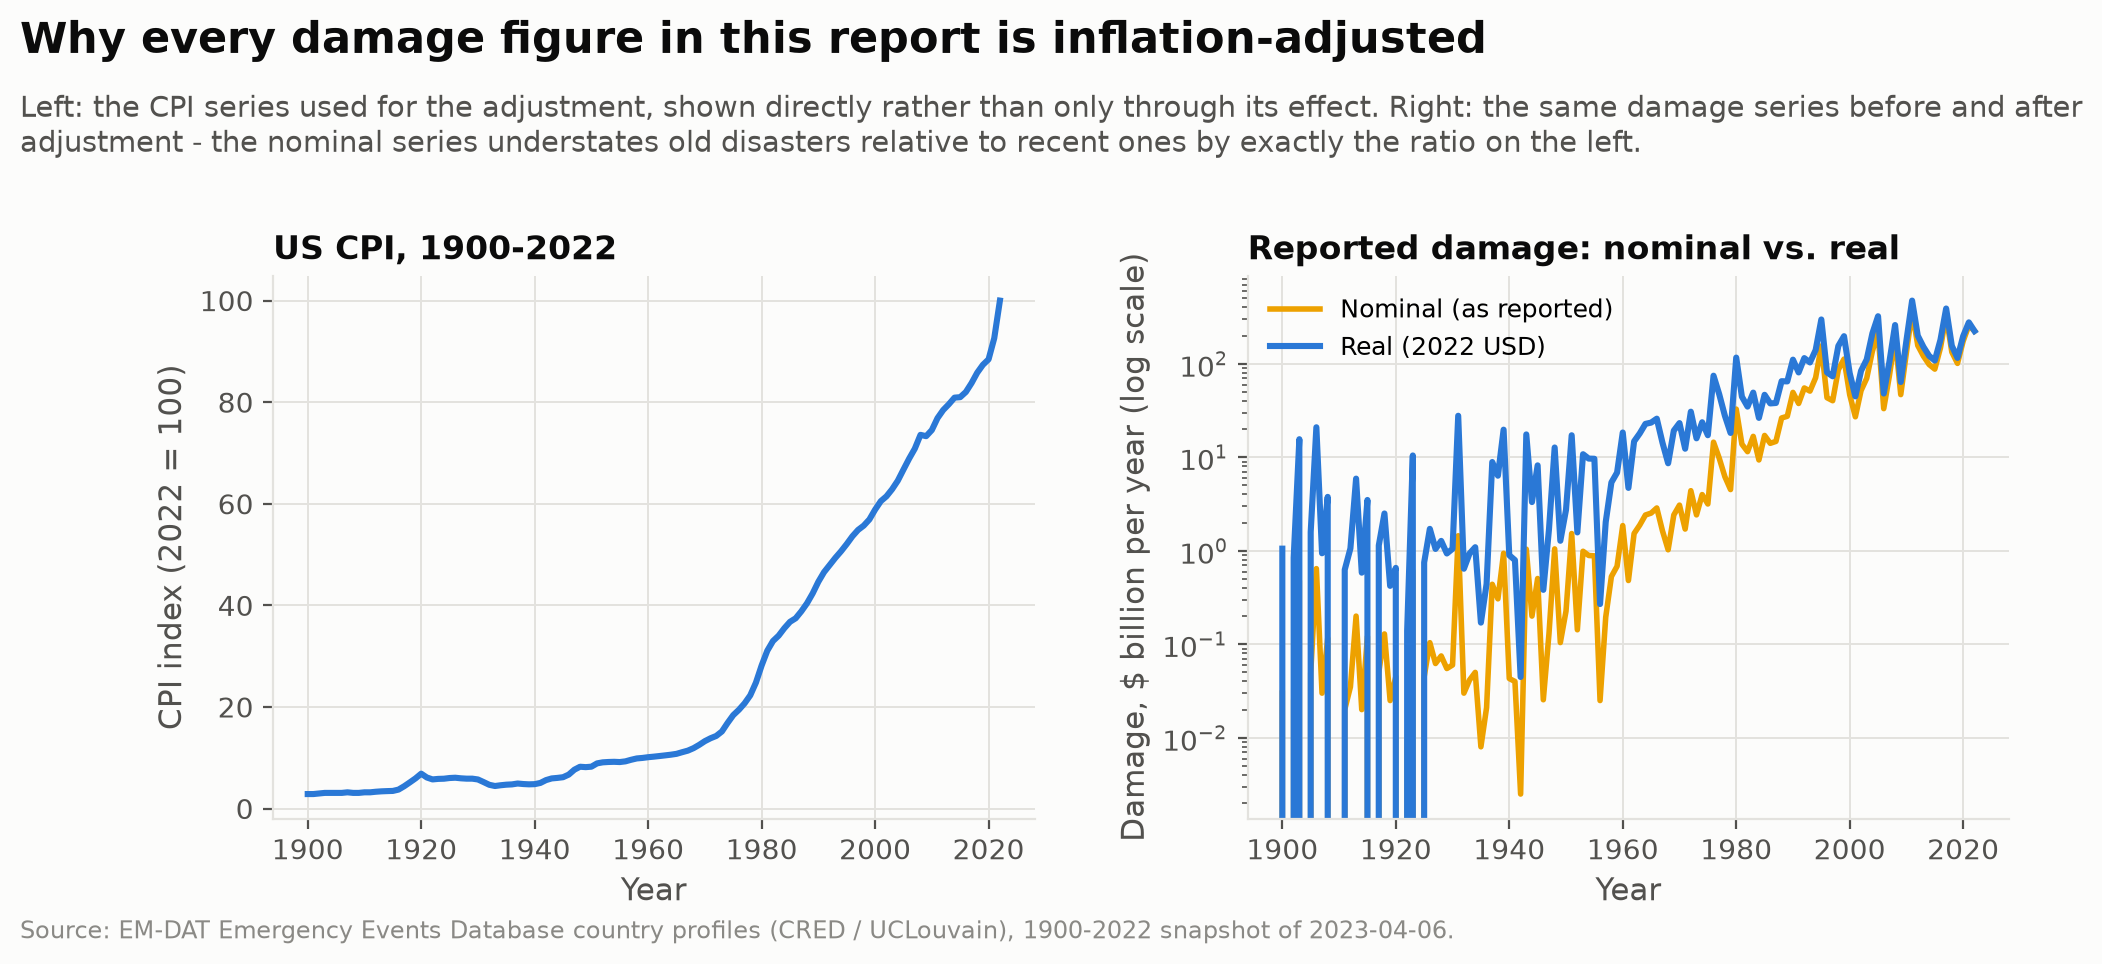
\includegraphics[width=\figw]{Fig21}
\caption[The CPI adjustment, shown directly]{\textbf{The inflation adjustment,
shown rather than asserted.} Section~\ref{sec:prep} states the adjustment as a
formula; this is what it does. It is also the only figure in the report that
uses the \texttt{CPI} column directly.}
\label{fig:cpi}
\end{figure}

\howto Left: the CPI index itself, 2.85 in 1900 rising to 100 in 2022 by
definition. Right: total reported damage per year drawn twice --- once as
originally reported (gold) and once in constant 2022 dollars (blue) --- on a log
axis. The vertical gap between the two lines at any year is exactly the CPI
ratio for that year.

\inference The gap is enormous early and closes to nothing by 2022, which is
why the nominal total (\$4.19 trillion) and the real total (\$6.70 trillion)
differ so much. Any damage trend drawn on nominal figures would be measuring
American inflation as much as disaster cost.

\begin{figure}[H]
\centering
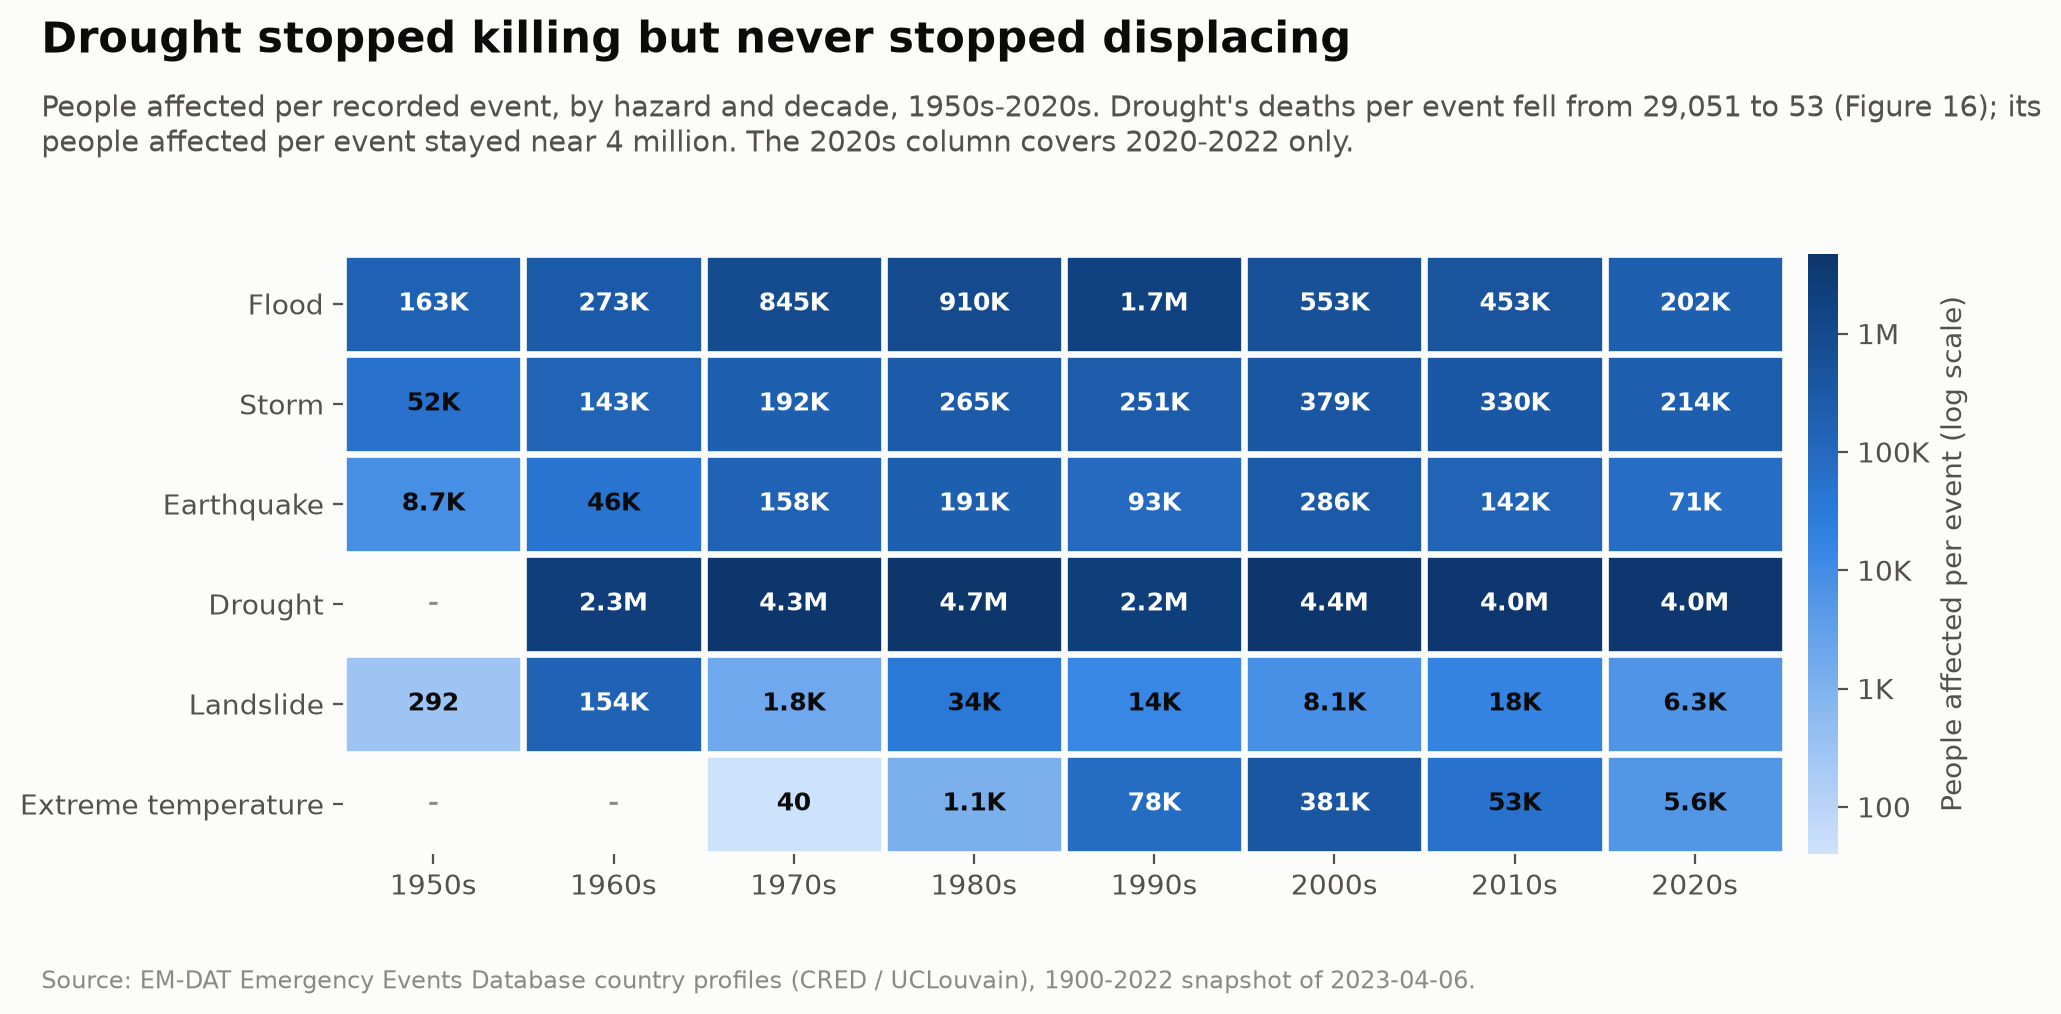
\includegraphics[width=\figw]{Fig22}
\caption[People affected per event, by hazard and decade]{\textbf{People
affected per recorded event, by hazard and decade.} Deliberately the same form,
hazards and decades as Figure~\ref{fig:heatmap}, with deaths swapped for people
affected, so the two can be read directly against each other.}
\label{fig:affected}
\end{figure}

\howto Identical construction to Figure~\ref{fig:heatmap}: rows are hazards,
columns decades, each cell prints its value, colour is a logarithmic blue ramp.
Only the measure has changed. Compare a cell here with the same cell there.

\inference This is the most important qualification in the report.
Figure~\ref{fig:heatmap} showed drought's deaths per event collapsing from
29{,}051 in the 1960s to 53 in the 2020s --- the single strongest piece of
evidence for the claim that vulnerability fell. But drought's \emph{people
affected} per event never fell: it sits near 4 million across every decade from
the 1970s on. Drought stopped killing people and carried on displacing them at
the same rate. The report's headline should therefore be read narrowly: what
fell is \emph{mortality} per event, not harm per event.

%=======================================================================
\section{Author Contributions}
\label{sec:contrib}
%=======================================================================

All three members contributed equally. Task sets were assigned as whole units ---
a member owns their sub-question, their figures, their inferences and their
section of this report and of the video --- so that no task is split across
members.

\subsection*{\memberA~(\rollA) --- Data processing lead and Task Set A (\emph{When?})}
Sourced the dataset and identified the delimiter/decimal and trailing-whitespace
issues; wrote the shared cleaning module \texttt{emdat\_common.py} including the
2023 part-year exclusion and the CPI-adjustment verification; produced the
Tableau-ready extract and the pipeline diagram (Figure~\ref{fig:pipeline});
designed and implemented Task Set A (Figures~\ref{fig:types}--\ref{fig:trimmed}),
including the reporting-bias diagnostic (Figure~\ref{fig:reporting}) and the
trimmed-deaths robustness test (Figure~\ref{fig:trimmed}) that qualified the
team's headline finding; wrote Sections 2, 3 and 4; presents the preprocessing
minute and Task Set A in the video.

\subsection*{\memberB~(\rollB) --- Task Set B (\emph{Where?})}
Designed and implemented Task Set B
(Figures~\ref{fig:mapevents}--\ref{fig:lethality}); built the Plotly choropleth
pipeline including the logarithmic colour scale and ISO-3 joins; produced the
four-panel country leaderboards, the concentration curves and the lethality
ranking; identified the events/deaths/damage rank mismatch (United States 1st
versus 23rd) that became a central thread of the data story; wrote Sections 5 and
9; presents Task Set B in the video.

\subsection*{\memberC~(\rollC) --- Task Set C (\emph{What?})}
Designed and implemented Task Set C
(Figures~\ref{fig:signature}--\ref{fig:decoupling}); built the hazard
impact-signature chart, the deadliness--cost plane, the real-damage time series,
the lethality heatmap and the indexed decoupling chart; ran the log-linear trend
fits and the Spearman decoupling test, and established that annual deaths carry
no significant post-1970 trend; found the rising extreme-temperature lethality;
wrote Sections 6 and 8; presents Task Set C in the video.

\subsection*{Jointly}
The guiding question and the three-way task decomposition
(Figure~\ref{fig:taskmap}); the visual design conventions of Section 3;
Sections 1, 7 and 10; the \LaTeX{} report template; the video storyboard; final
review.


%=======================================================================
\section{AI Declaration Forms}
\label{sec:ai}
%=======================================================================

One signed declaration per team member follows, on the form circulated by the
course instructor, as required by the assignment brief.

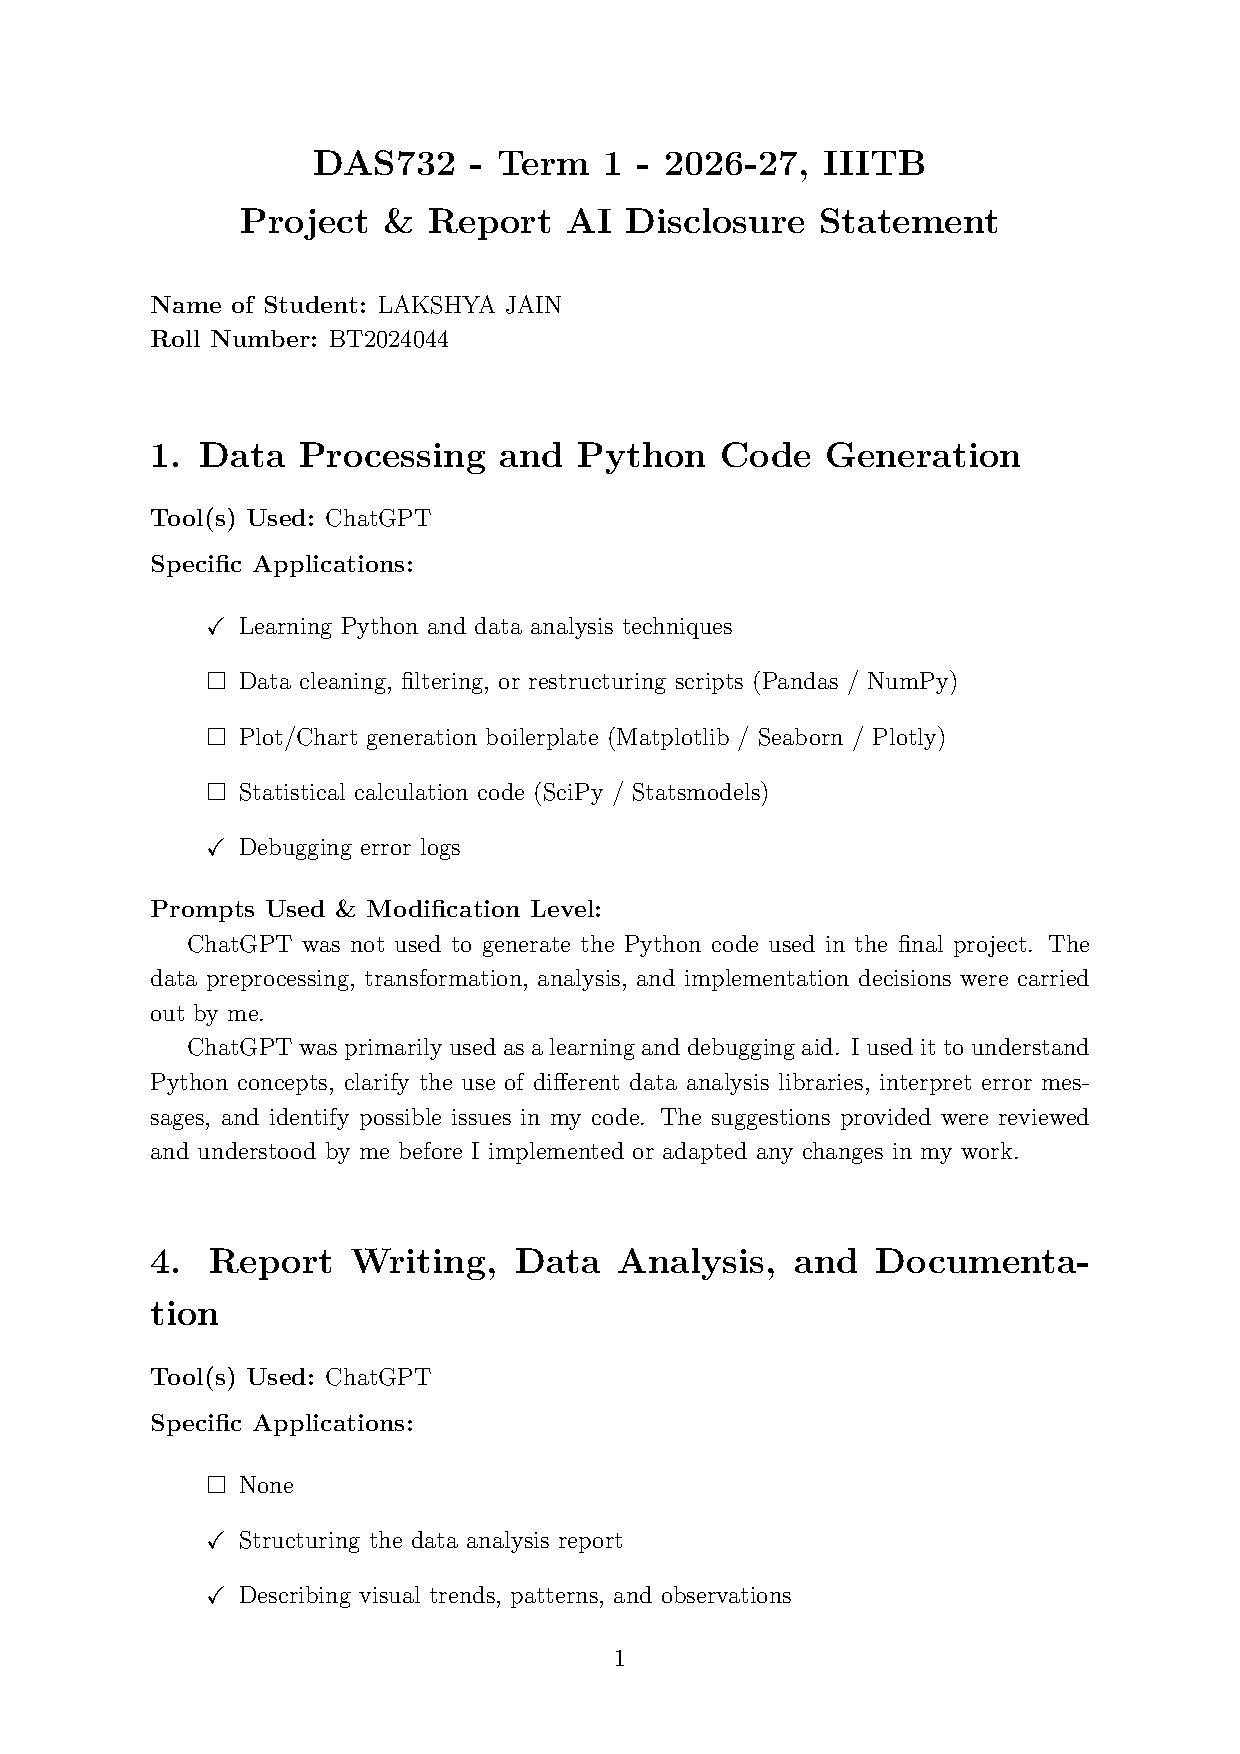
\includepdf[pages=-,fitpaper=false,width=\textwidth,
            pagecommand={\thispagestyle{fancy}}]{../ai_disclosures/AI_Declaration_Lakshya_Jain_BT2024044.pdf}
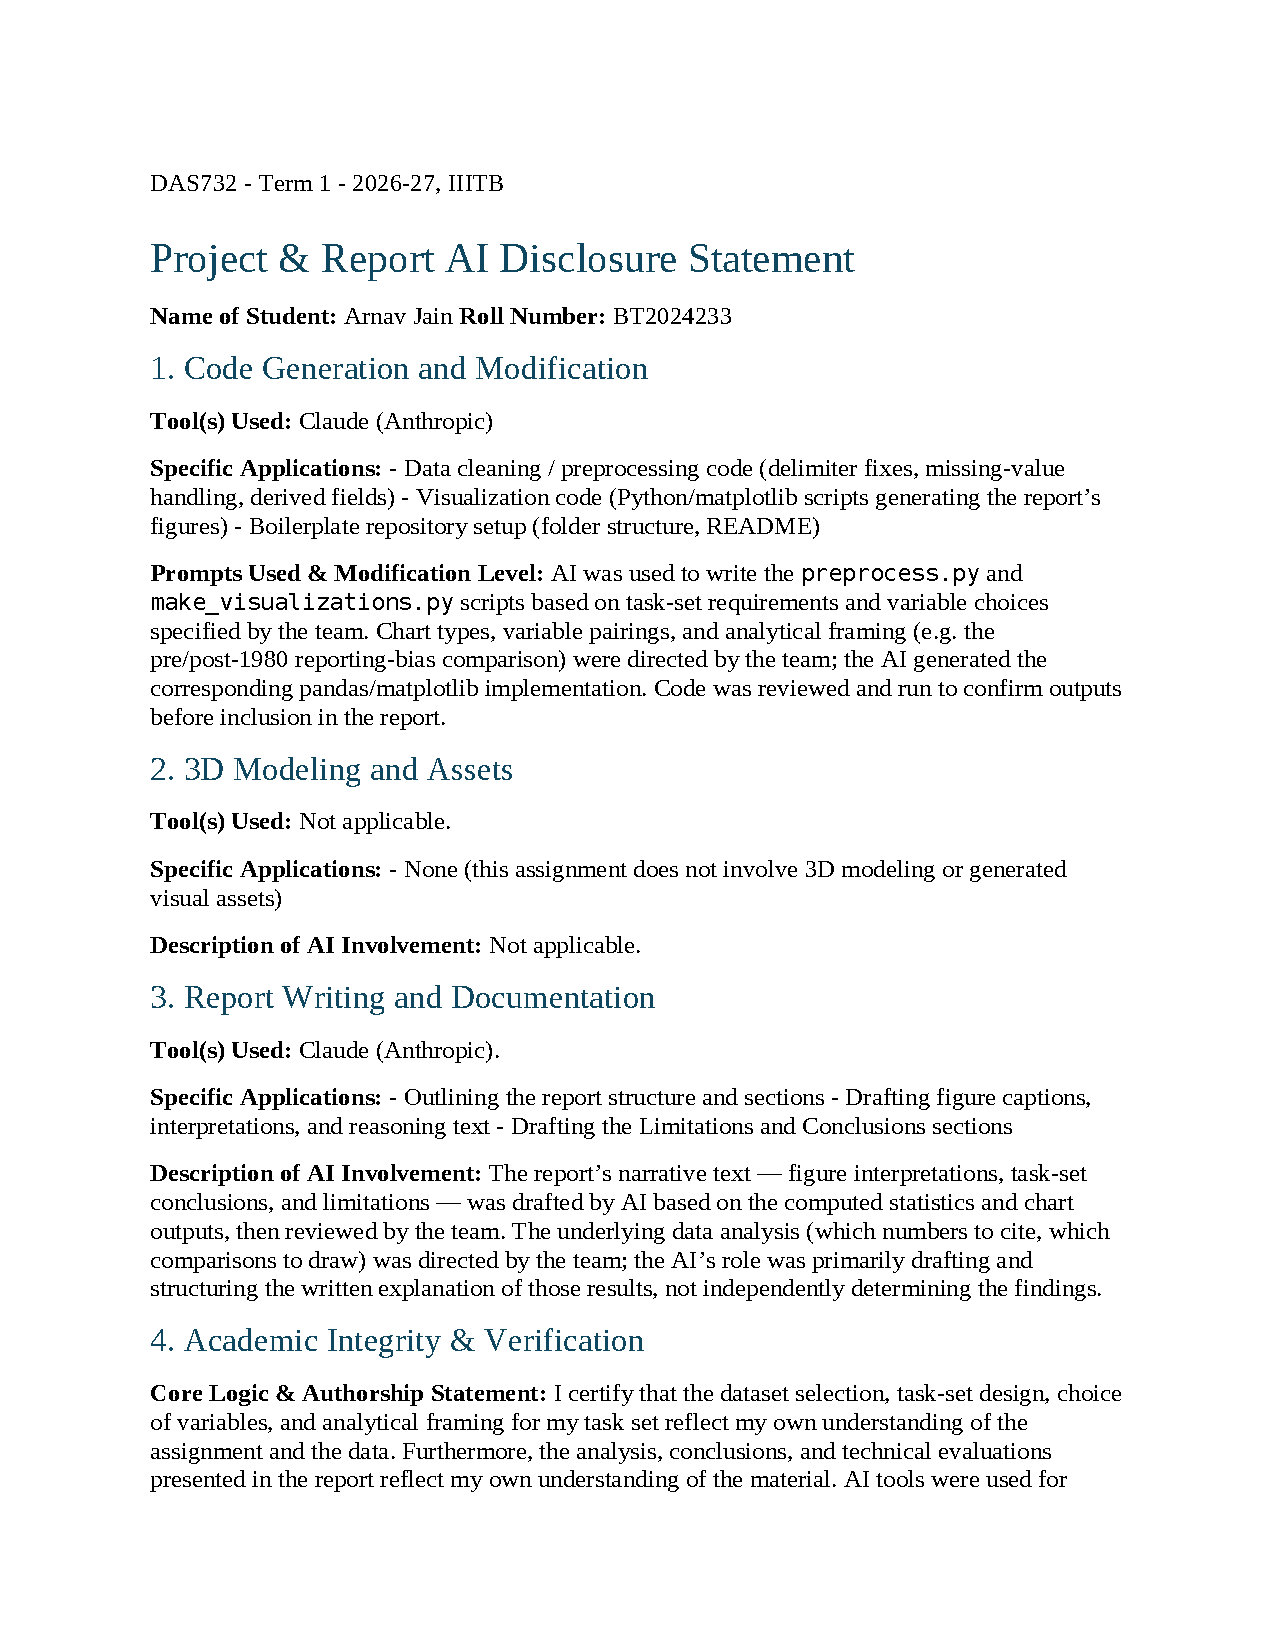
\includepdf[pages=-,fitpaper=false,width=\textwidth,
            pagecommand={\thispagestyle{fancy}}]{../ai_disclosures/AI_Declaration_Arnav_Jain_BT2024233.pdf}
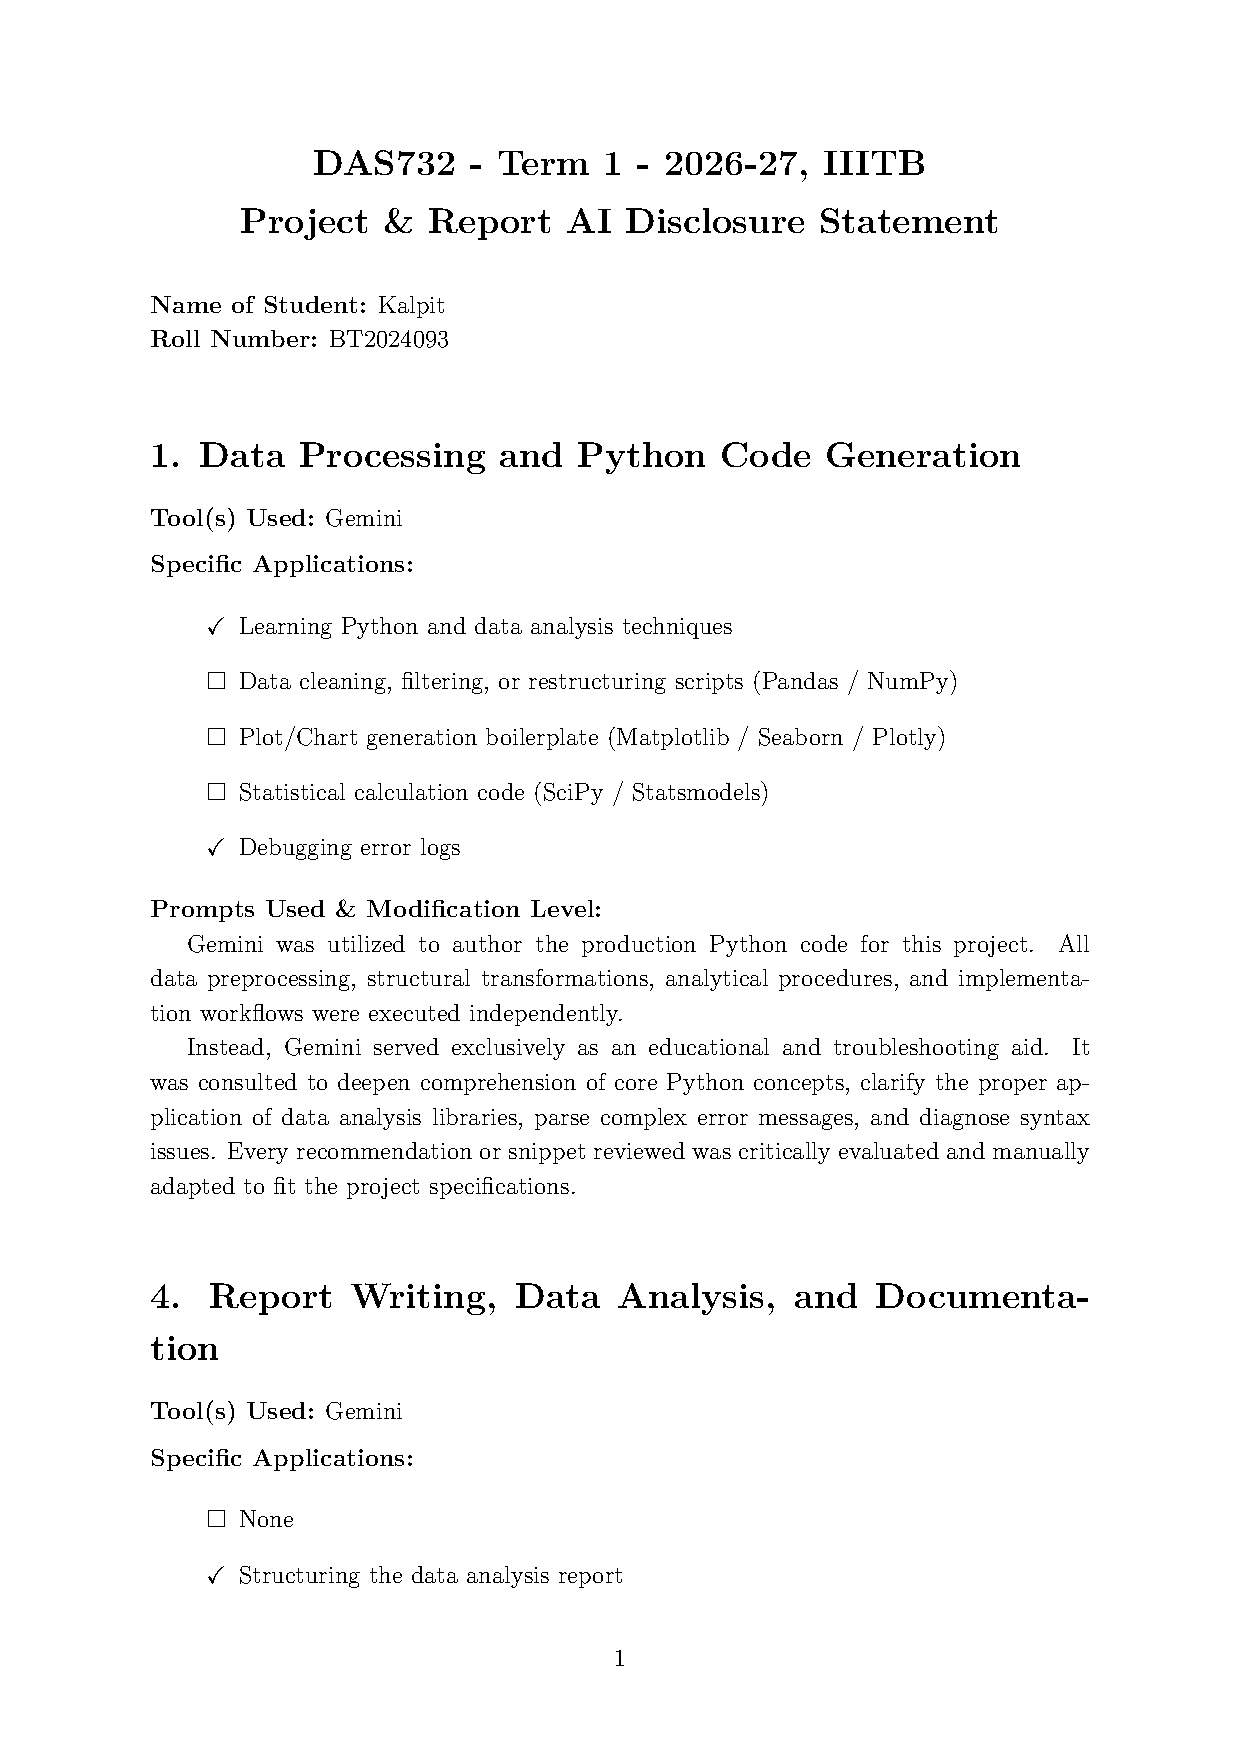
\includepdf[pages=-,fitpaper=false,width=\textwidth,
            pagecommand={\thispagestyle{fancy}}]{../ai_disclosures/AI_Declaration_Kalpit_BT2024093.pdf}

%=======================================================================
\begin{thebibliography}{9}
\bibitem{schulz2013}
H.-J. Schulz, T. Nocke, M. Heitzler and H. Schumann,
``A design space of visualization tasks,''
\emph{IEEE Transactions on Visualization and Computer Graphics},
vol.~19, no.~12, pp.~2366--2375, 2013.

\bibitem{emdat}
Centre for Research on the Epidemiology of Disasters (CRED), UCLouvain,
\emph{EM-DAT: The International Disaster Database}.
\url{https://www.emdat.be}

\bibitem{kaggle}
Kaggle dataset mirror, \emph{Natural Disasters Emergency Events Database}.
\url{https://www.kaggle.com/datasets/mexwell/natural-disasters-emergency-events-database}
\end{thebibliography}

\end{document}
